\documentclass[twoside]{book}

% Packages required by doxygen
\usepackage{fixltx2e}
\usepackage{calc}
\usepackage{doxygen}
\usepackage[export]{adjustbox} % also loads graphicx
\usepackage{graphicx}
\usepackage[utf8]{inputenc}
\usepackage{makeidx}
\usepackage{multicol}
\usepackage{multirow}
\PassOptionsToPackage{warn}{textcomp}
\usepackage{textcomp}
\usepackage[nointegrals]{wasysym}
\usepackage[table]{xcolor}

% Font selection
\usepackage[T1]{fontenc}
\usepackage[scaled=.90]{helvet}
\usepackage{courier}
\usepackage{amssymb}
\usepackage{sectsty}
\renewcommand{\familydefault}{\sfdefault}
\allsectionsfont{%
  \fontseries{bc}\selectfont%
  \color{darkgray}%
}
\renewcommand{\DoxyLabelFont}{%
  \fontseries{bc}\selectfont%
  \color{darkgray}%
}
\newcommand{\+}{\discretionary{\mbox{\scriptsize$\hookleftarrow$}}{}{}}

% Page & text layout
\usepackage{geometry}
\geometry{%
  a4paper,%
  top=2.5cm,%
  bottom=2.5cm,%
  left=2.5cm,%
  right=2.5cm%
}
\tolerance=750
\hfuzz=15pt
\hbadness=750
\setlength{\emergencystretch}{15pt}
\setlength{\parindent}{0cm}
\setlength{\parskip}{3ex plus 2ex minus 2ex}
\makeatletter
\renewcommand{\paragraph}{%
  \@startsection{paragraph}{4}{0ex}{-1.0ex}{1.0ex}{%
    \normalfont\normalsize\bfseries\SS@parafont%
  }%
}
\renewcommand{\subparagraph}{%
  \@startsection{subparagraph}{5}{0ex}{-1.0ex}{1.0ex}{%
    \normalfont\normalsize\bfseries\SS@subparafont%
  }%
}
\makeatother

% Headers & footers
\usepackage{fancyhdr}
\pagestyle{fancyplain}
\fancyhead[LE]{\fancyplain{}{\bfseries\thepage}}
\fancyhead[CE]{\fancyplain{}{}}
\fancyhead[RE]{\fancyplain{}{\bfseries\leftmark}}
\fancyhead[LO]{\fancyplain{}{\bfseries\rightmark}}
\fancyhead[CO]{\fancyplain{}{}}
\fancyhead[RO]{\fancyplain{}{\bfseries\thepage}}
\fancyfoot[LE]{\fancyplain{}{}}
\fancyfoot[CE]{\fancyplain{}{}}
\fancyfoot[RE]{\fancyplain{}{\bfseries\scriptsize Generated by Doxygen }}
\fancyfoot[LO]{\fancyplain{}{\bfseries\scriptsize Generated by Doxygen }}
\fancyfoot[CO]{\fancyplain{}{}}
\fancyfoot[RO]{\fancyplain{}{}}
\renewcommand{\footrulewidth}{0.4pt}
\renewcommand{\chaptermark}[1]{%
  \markboth{#1}{}%
}
\renewcommand{\sectionmark}[1]{%
  \markright{\thesection\ #1}%
}

% Indices & bibliography
\usepackage{natbib}
\usepackage[titles]{tocloft}
\setcounter{tocdepth}{3}
\setcounter{secnumdepth}{5}
\makeindex

% Hyperlinks (required, but should be loaded last)
\usepackage{ifpdf}
\ifpdf
  \usepackage[pdftex,pagebackref=true]{hyperref}
\else
  \usepackage[ps2pdf,pagebackref=true]{hyperref}
\fi
\hypersetup{%
  colorlinks=true,%
  linkcolor=blue,%
  citecolor=blue,%
  unicode%
}

% Custom commands
\newcommand{\clearemptydoublepage}{%
  \newpage{\pagestyle{empty}\cleardoublepage}%
}

\usepackage{caption}
\captionsetup{labelsep=space,justification=centering,font={bf},singlelinecheck=off,skip=4pt,position=top}

%===== C O N T E N T S =====

\begin{document}

% Titlepage & ToC
\hypersetup{pageanchor=false,
             bookmarksnumbered=true,
             pdfencoding=unicode
            }
\pagenumbering{alph}
\begin{titlepage}
\vspace*{7cm}
\begin{center}%
{\Large Quantum computing }\\
\vspace*{1cm}
{\large Generated by Doxygen 1.8.13}\\
\end{center}
\end{titlepage}
\clearemptydoublepage
\pagenumbering{roman}
\tableofcontents
\clearemptydoublepage
\pagenumbering{arabic}
\hypersetup{pageanchor=true}

%--- Begin generated contents ---
\chapter{CS 5201 Assignment 6}
\label{md_README}
\Hypertarget{md_README}
Read the directions on the \href{https://jberm6.git-pages.mst.edu/essman/homework/hw6/}{\tt course website}

\subsubsection*{Automated Tests}

Because (like assignment 4), this assignment is fairly open-\/ended, no unit tests will be provided. More information on validating your driver results will be provided on the assignment page. 
\chapter{Class Index}
\section{Class List}
Here are the classes, structs, unions and interfaces with brief descriptions\+:\begin{DoxyCompactList}
\item\contentsline{section}{\hyperlink{classcomplex}{complex$<$ T $>$} \\*Complex class }{\pageref{classcomplex}}{}
\item\contentsline{section}{\hyperlink{classgatedata}{gatedata} \\*Complex class }{\pageref{classgatedata}}{}
\item\contentsline{section}{\hyperlink{classnVect_1_1iterator}{n\+Vect$<$ T $>$\+::iterator} \\*Iterator class }{\pageref{classnVect_1_1iterator}}{}
\item\contentsline{section}{\hyperlink{classkronecker}{kronecker$<$ T $>$} \\*Kronecker class }{\pageref{classkronecker}}{}
\item\contentsline{section}{\hyperlink{classnTrix}{n\+Trix$<$ T $>$} \\*N\+Trix class }{\pageref{classnTrix}}{}
\item\contentsline{section}{\hyperlink{classnVect}{n\+Vect$<$ T $>$} \\*N\+Vect class }{\pageref{classnVect}}{}
\item\contentsline{section}{\hyperlink{classqreg}{qreg$<$ size $>$} \\*Qreg class }{\pageref{classqreg}}{}
\end{DoxyCompactList}

\chapter{File Index}
\section{File List}
Here is a list of all documented files with brief descriptions\+:\begin{DoxyCompactList}
\item\contentsline{section}{\hyperlink{complex_8h}{complex.\+h} }{\pageref{complex_8h}}{}
\item\contentsline{section}{{\bfseries complex.\+hpp} }{\pageref{complex_8hpp}}{}
\item\contentsline{section}{\hyperlink{gatedata_8h}{gatedata.\+h} }{\pageref{gatedata_8h}}{}
\item\contentsline{section}{\hyperlink{kronecker_8h}{kronecker.\+h} }{\pageref{kronecker_8h}}{}
\item\contentsline{section}{{\bfseries kronecker.\+hpp} }{\pageref{kronecker_8hpp}}{}
\item\contentsline{section}{\hyperlink{nTrix_8h}{n\+Trix.\+h} }{\pageref{nTrix_8h}}{}
\item\contentsline{section}{{\bfseries n\+Trix.\+hpp} }{\pageref{nTrix_8hpp}}{}
\item\contentsline{section}{\hyperlink{nVect_8h}{n\+Vect.\+h} }{\pageref{nVect_8h}}{}
\item\contentsline{section}{{\bfseries n\+Vect.\+hpp} }{\pageref{nVect_8hpp}}{}
\item\contentsline{section}{\hyperlink{qreg_8h}{qreg.\+h} }{\pageref{qreg_8h}}{}
\item\contentsline{section}{{\bfseries qreg.\+hpp} }{\pageref{qreg_8hpp}}{}
\end{DoxyCompactList}

\chapter{Class Documentation}
\hypertarget{classcomplex}{}\section{complex$<$ T $>$ Class Template Reference}
\label{classcomplex}\index{complex$<$ T $>$@{complex$<$ T $>$}}


complex class.  




{\ttfamily \#include $<$complex.\+h$>$}

\subsection*{Public Member Functions}
\begin{DoxyCompactItemize}
\item 
\hyperlink{classcomplex_a9752049742449cbc9571cd8f183f72b2}{complex} ()
\begin{DoxyCompactList}\small\item\em Constructor. \end{DoxyCompactList}\item 
\hyperlink{classcomplex_a27a5d75c2060b32de98ae4666fd691d1}{complex} (const T \&a, const T \&b)
\begin{DoxyCompactList}\small\item\em Constructor. \end{DoxyCompactList}\item 
\hyperlink{classcomplex_aca6c030056b5e089883c5e64a0309c28}{complex} (const \hyperlink{classcomplex}{complex} \&rhs)
\begin{DoxyCompactList}\small\item\em Copy Constructor. \end{DoxyCompactList}\item 
\hyperlink{classcomplex}{complex} \& \hyperlink{classcomplex_a67d65378570f4b7a158b14a1502cc75f}{operator=} (const \hyperlink{classcomplex}{complex} \&rhs)
\begin{DoxyCompactList}\small\item\em = operator \end{DoxyCompactList}\item 
\hyperlink{classcomplex_a949d63a288cccf405266874f95357815}{$\sim$complex} ()
\begin{DoxyCompactList}\small\item\em Destructor. \end{DoxyCompactList}\item 
T \hyperlink{classcomplex_a9e88306cc536506d0370b7376e40287b}{real} () const
\begin{DoxyCompactList}\small\item\em Real Accessor. \end{DoxyCompactList}\item 
T \hyperlink{classcomplex_a4edf203a6e7005a5d6817473d703a423}{imag} () const
\begin{DoxyCompactList}\small\item\em Imaginary Accessor. \end{DoxyCompactList}\item 
\hyperlink{classcomplex}{complex}$<$ T $>$ \hyperlink{classcomplex_abef23308534cc50484e7d154a8497dbc}{operator-\/} () const
\begin{DoxyCompactList}\small\item\em Additive Inverse. \end{DoxyCompactList}\item 
\hyperlink{classcomplex}{complex}$<$ T $>$ \hyperlink{classcomplex_a0a6eb0b21f6f7d0084c7edc637e98e10}{operator!} () const
\begin{DoxyCompactList}\small\item\em Complex Conjugate. \end{DoxyCompactList}\item 
T \hyperlink{classcomplex_a53710ae99345025cc52a6ecc1804cb8d}{operator$\sim$} () const
\begin{DoxyCompactList}\small\item\em Magnitude. \end{DoxyCompactList}\item 
\hyperlink{classcomplex}{complex}$<$ T $>$ \hyperlink{classcomplex_aa10f3dbe0731c90d1b15408e3f11ae52}{operator+} (const \hyperlink{classcomplex}{complex}$<$ T $>$ \&rhs) const
\begin{DoxyCompactList}\small\item\em Addition. \end{DoxyCompactList}\item 
\hyperlink{classcomplex}{complex}$<$ T $>$ \hyperlink{classcomplex_a7f61f4a380f418de039d1f65946424ef}{operator-\/} (const \hyperlink{classcomplex}{complex}$<$ T $>$ \&rhs) const
\begin{DoxyCompactList}\small\item\em Subtraction. \end{DoxyCompactList}\item 
\hyperlink{classcomplex}{complex}$<$ T $>$ \hyperlink{classcomplex_ad2f08f4f8eea0ef2def536898addd7f3}{operator$\ast$} (const \hyperlink{classcomplex}{complex}$<$ T $>$ \&rhs) const
\begin{DoxyCompactList}\small\item\em Multiplication. \end{DoxyCompactList}\item 
\hyperlink{classcomplex}{complex}$<$ T $>$ \& \hyperlink{classcomplex_a0e0def25b2e4c7da5c8e845132560d2b}{operator=} (const int number)
\begin{DoxyCompactList}\small\item\em Integer = operator. \end{DoxyCompactList}\item 
\hyperlink{classcomplex}{complex}$<$ T $>$ \& \hyperlink{classcomplex_addf9684dc875ae196619c9fadd5fe48e}{operator+=} (const \hyperlink{classcomplex}{complex}$<$ T $>$ \&rhs)
\begin{DoxyCompactList}\small\item\em += operator \end{DoxyCompactList}\item 
\hyperlink{classcomplex}{complex}$<$ T $>$ \& \hyperlink{classcomplex_a272e86ba6de2f88cb1803127f8ff0481}{operator-\/=} (const \hyperlink{classcomplex}{complex}$<$ T $>$ \&rhs)
\begin{DoxyCompactList}\small\item\em -\/= operator \end{DoxyCompactList}\item 
\hyperlink{classcomplex}{complex}$<$ T $>$ \& \hyperlink{classcomplex_a98240d564a6667f9acf5163821365cdc}{operator$\ast$=} (const \hyperlink{classcomplex}{complex}$<$ T $>$ \&rhs)
\begin{DoxyCompactList}\small\item\em $\ast$= operator \end{DoxyCompactList}\end{DoxyCompactItemize}
\subsection*{Friends}
\begin{DoxyCompactItemize}
\item 
{\footnotesize template$<$typename U $>$ }\\std\+::ostream \& \hyperlink{classcomplex_a860d572e8b354fd76998c8c1309754f9}{operator$<$$<$} (std\+::ostream \&out, const \hyperlink{classcomplex}{complex}$<$ U $>$ \&rhs)
\begin{DoxyCompactList}\small\item\em Insertion operator. \end{DoxyCompactList}\end{DoxyCompactItemize}


\subsection{Detailed Description}
\subsubsection*{template$<$typename T$>$\newline
class complex$<$ T $>$}

complex class. 

This class uses two type T objects to store and represent a complex number. 

\subsection{Constructor \& Destructor Documentation}
\mbox{\Hypertarget{classcomplex_a9752049742449cbc9571cd8f183f72b2}\label{classcomplex_a9752049742449cbc9571cd8f183f72b2}} 
\index{complex@{complex}!complex@{complex}}
\index{complex@{complex}!complex@{complex}}
\subsubsection{\texorpdfstring{complex()}{complex()}\hspace{0.1cm}{\footnotesize\ttfamily [1/3]}}
{\footnotesize\ttfamily template$<$typename T$>$ \\
\hyperlink{classcomplex}{complex}$<$ T $>$\+::\hyperlink{classcomplex}{complex} (\begin{DoxyParamCaption}{ }\end{DoxyParamCaption})\hspace{0.3cm}{\ttfamily [inline]}}



Constructor. 

Description\+: Default constructor for the complex class that initializes the real value as 1 and the imaginary value as 0. \begin{DoxyPostcond}{Postcondition}
A complex number is initialized with the values specified. 
\end{DoxyPostcond}
\mbox{\Hypertarget{classcomplex_a27a5d75c2060b32de98ae4666fd691d1}\label{classcomplex_a27a5d75c2060b32de98ae4666fd691d1}} 
\index{complex@{complex}!complex@{complex}}
\index{complex@{complex}!complex@{complex}}
\subsubsection{\texorpdfstring{complex()}{complex()}\hspace{0.1cm}{\footnotesize\ttfamily [2/3]}}
{\footnotesize\ttfamily template$<$typename T$>$ \\
\hyperlink{classcomplex}{complex}$<$ T $>$\+::\hyperlink{classcomplex}{complex} (\begin{DoxyParamCaption}\item[{const T \&}]{a,  }\item[{const T \&}]{b }\end{DoxyParamCaption})\hspace{0.3cm}{\ttfamily [inline]}}



Constructor. 

Description\+: Parameterized constructor for the complex class that initializes the different parts with the values passed. 
\begin{DoxyParams}{Parameters}
{\em a} & is the real value for the complex number. \\
\hline
{\em b} & is the imaginary value for the complex number. \\
\hline
\end{DoxyParams}
\begin{DoxyPostcond}{Postcondition}
A complex number is initialized with the values passed. 
\end{DoxyPostcond}
\mbox{\Hypertarget{classcomplex_aca6c030056b5e089883c5e64a0309c28}\label{classcomplex_aca6c030056b5e089883c5e64a0309c28}} 
\index{complex@{complex}!complex@{complex}}
\index{complex@{complex}!complex@{complex}}
\subsubsection{\texorpdfstring{complex()}{complex()}\hspace{0.1cm}{\footnotesize\ttfamily [3/3]}}
{\footnotesize\ttfamily template$<$typename T$>$ \\
\hyperlink{classcomplex}{complex}$<$ T $>$\+::\hyperlink{classcomplex}{complex} (\begin{DoxyParamCaption}\item[{const \hyperlink{classcomplex}{complex}$<$ T $>$ \&}]{rhs }\end{DoxyParamCaption})}



Copy Constructor. 

Description\+: A copy constructor for the complex class that initializes a new complex object with the values of the complex object passed. 
\begin{DoxyParams}{Parameters}
{\em rhs} & is the complex object to be copied. \\
\hline
\end{DoxyParams}
\begin{DoxyPrecond}{Precondition}
operator = must be defined for type T. 
\end{DoxyPrecond}
\begin{DoxyPostcond}{Postcondition}
A complex number is initialized with the same values as the object passed. 
\end{DoxyPostcond}
\mbox{\Hypertarget{classcomplex_a949d63a288cccf405266874f95357815}\label{classcomplex_a949d63a288cccf405266874f95357815}} 
\index{complex@{complex}!````~complex@{$\sim$complex}}
\index{````~complex@{$\sim$complex}!complex@{complex}}
\subsubsection{\texorpdfstring{$\sim$complex()}{~complex()}}
{\footnotesize\ttfamily template$<$typename T$>$ \\
\hyperlink{classcomplex}{complex}$<$ T $>$\+::$\sim$\hyperlink{classcomplex}{complex} (\begin{DoxyParamCaption}{ }\end{DoxyParamCaption})\hspace{0.3cm}{\ttfamily [inline]}}



Destructor. 

Description\+: Placeholder function for complex destructor. \begin{DoxyPostcond}{Postcondition}
The calling object is safely desctructed. 
\end{DoxyPostcond}


\subsection{Member Function Documentation}
\mbox{\Hypertarget{classcomplex_a4edf203a6e7005a5d6817473d703a423}\label{classcomplex_a4edf203a6e7005a5d6817473d703a423}} 
\index{complex@{complex}!imag@{imag}}
\index{imag@{imag}!complex@{complex}}
\subsubsection{\texorpdfstring{imag()}{imag()}}
{\footnotesize\ttfamily template$<$typename T $>$ \\
T \hyperlink{classcomplex}{complex}$<$ T $>$\+::imag (\begin{DoxyParamCaption}{ }\end{DoxyParamCaption}) const}



Imaginary Accessor. 

Description\+: Accessor for the imaginary member for the complex class that returns a copy of the imaginary part of the calling object. \begin{DoxyReturn}{Returns}
Returns a copy of m\+\_\+b from the calling object. 
\end{DoxyReturn}
\mbox{\Hypertarget{classcomplex_a0a6eb0b21f6f7d0084c7edc637e98e10}\label{classcomplex_a0a6eb0b21f6f7d0084c7edc637e98e10}} 
\index{complex@{complex}!operator"!@{operator"!}}
\index{operator"!@{operator"!}!complex@{complex}}
\subsubsection{\texorpdfstring{operator"!()}{operator!()}}
{\footnotesize\ttfamily template$<$typename T $>$ \\
\hyperlink{classcomplex}{complex}$<$ T $>$ \hyperlink{classcomplex}{complex}$<$ T $>$\+::operator! (\begin{DoxyParamCaption}{ }\end{DoxyParamCaption}) const}



Complex Conjugate. 

Description\+: Returns the complex conjugate of the calling object. -\/m\+\_\+b. \begin{DoxyReturn}{Returns}
Returns a T object that represents the complex conjugate of the complex number. 
\end{DoxyReturn}
\begin{DoxyPrecond}{Precondition}
unary -\/ operator must be defined for type T. 
\end{DoxyPrecond}
\mbox{\Hypertarget{classcomplex_ad2f08f4f8eea0ef2def536898addd7f3}\label{classcomplex_ad2f08f4f8eea0ef2def536898addd7f3}} 
\index{complex@{complex}!operator$\ast$@{operator$\ast$}}
\index{operator$\ast$@{operator$\ast$}!complex@{complex}}
\subsubsection{\texorpdfstring{operator$\ast$()}{operator*()}}
{\footnotesize\ttfamily template$<$typename T$>$ \\
\hyperlink{classcomplex}{complex}$<$ T $>$ \hyperlink{classcomplex}{complex}$<$ T $>$\+::operator$\ast$ (\begin{DoxyParamCaption}\item[{const \hyperlink{classcomplex}{complex}$<$ T $>$ \&}]{rhs }\end{DoxyParamCaption}) const}



Multiplication. 

Description\+: Binary $\ast$ operator for the complex class that calculates the product of the two complex objects. 
\begin{DoxyParams}{Parameters}
{\em rhs} & is the complex object to be multiplied to the calling object. \\
\hline
\end{DoxyParams}
\begin{DoxyReturn}{Returns}
Returns a complex object that represents the product of the two complex objects. 
\end{DoxyReturn}
\begin{DoxyPrecond}{Precondition}
Binary $\ast$ operator, Binary + operator, and unary -\/ operator must be defined for type T. 
\end{DoxyPrecond}
\mbox{\Hypertarget{classcomplex_a98240d564a6667f9acf5163821365cdc}\label{classcomplex_a98240d564a6667f9acf5163821365cdc}} 
\index{complex@{complex}!operator$\ast$=@{operator$\ast$=}}
\index{operator$\ast$=@{operator$\ast$=}!complex@{complex}}
\subsubsection{\texorpdfstring{operator$\ast$=()}{operator*=()}}
{\footnotesize\ttfamily template$<$typename T$>$ \\
\hyperlink{classcomplex}{complex}$<$ T $>$ \& \hyperlink{classcomplex}{complex}$<$ T $>$\+::operator$\ast$= (\begin{DoxyParamCaption}\item[{const \hyperlink{classcomplex}{complex}$<$ T $>$ \&}]{rhs }\end{DoxyParamCaption})}



$\ast$= operator 

Description\+: $\ast$= operator overload to increase functionality with the \hyperlink{classnTrix}{n\+Trix} (and other) classes. 
\begin{DoxyParams}{Parameters}
{\em rhs} & is the complex number to multiply to the calling object. \\
\hline
\end{DoxyParams}
\begin{DoxyReturn}{Returns}
Returns $\ast$this with modified data 
\end{DoxyReturn}
\begin{DoxyPrecond}{Precondition}
Binary $\ast$ operator, and = operator must be defined for type T. 
\end{DoxyPrecond}
\begin{DoxyPostcond}{Postcondition}
The calling object has the parameter multiplied to it. 
\end{DoxyPostcond}
\mbox{\Hypertarget{classcomplex_aa10f3dbe0731c90d1b15408e3f11ae52}\label{classcomplex_aa10f3dbe0731c90d1b15408e3f11ae52}} 
\index{complex@{complex}!operator+@{operator+}}
\index{operator+@{operator+}!complex@{complex}}
\subsubsection{\texorpdfstring{operator+()}{operator+()}}
{\footnotesize\ttfamily template$<$typename T$>$ \\
\hyperlink{classcomplex}{complex}$<$ T $>$ \hyperlink{classcomplex}{complex}$<$ T $>$\+::operator+ (\begin{DoxyParamCaption}\item[{const \hyperlink{classcomplex}{complex}$<$ T $>$ \&}]{rhs }\end{DoxyParamCaption}) const}



Addition. 

Description\+: Binary + operator for the complex class that calculates the addition of two complex objects. 
\begin{DoxyParams}{Parameters}
{\em rhs} & is the complex object to be added to the calling object. \\
\hline
\end{DoxyParams}
\begin{DoxyReturn}{Returns}
Returns a complex object that represents the addition of the two complex objects. 
\end{DoxyReturn}
\begin{DoxyPrecond}{Precondition}
Binary += operator must be defined for type T. 
\end{DoxyPrecond}
\mbox{\Hypertarget{classcomplex_addf9684dc875ae196619c9fadd5fe48e}\label{classcomplex_addf9684dc875ae196619c9fadd5fe48e}} 
\index{complex@{complex}!operator+=@{operator+=}}
\index{operator+=@{operator+=}!complex@{complex}}
\subsubsection{\texorpdfstring{operator+=()}{operator+=()}}
{\footnotesize\ttfamily template$<$typename T$>$ \\
\hyperlink{classcomplex}{complex}$<$ T $>$ \& \hyperlink{classcomplex}{complex}$<$ T $>$\+::operator+= (\begin{DoxyParamCaption}\item[{const \hyperlink{classcomplex}{complex}$<$ T $>$ \&}]{rhs }\end{DoxyParamCaption})}



+= operator 

Description\+: += operator overload to increase functionality with the \hyperlink{classnTrix}{n\+Trix} (and other) classes. 
\begin{DoxyParams}{Parameters}
{\em rhs} & is the complex number to add to the calling object. \\
\hline
\end{DoxyParams}
\begin{DoxyReturn}{Returns}
Returns $\ast$this with modified data 
\end{DoxyReturn}
\begin{DoxyPrecond}{Precondition}
Binary + operator, and = operator must be defined for type T. 
\end{DoxyPrecond}
\begin{DoxyPostcond}{Postcondition}
The calling object has the parameter added to it. 
\end{DoxyPostcond}
\mbox{\Hypertarget{classcomplex_abef23308534cc50484e7d154a8497dbc}\label{classcomplex_abef23308534cc50484e7d154a8497dbc}} 
\index{complex@{complex}!operator-\/@{operator-\/}}
\index{operator-\/@{operator-\/}!complex@{complex}}
\subsubsection{\texorpdfstring{operator-\/()}{operator-()}\hspace{0.1cm}{\footnotesize\ttfamily [1/2]}}
{\footnotesize\ttfamily template$<$typename T $>$ \\
\hyperlink{classcomplex}{complex}$<$ T $>$ \hyperlink{classcomplex}{complex}$<$ T $>$\+::operator-\/ (\begin{DoxyParamCaption}{ }\end{DoxyParamCaption}) const}



Additive Inverse. 

Description\+: Returns the additive inverse of the calling object. -\/m\+\_\+a. \begin{DoxyReturn}{Returns}
Returns a T object that represents the additive inverse of the complex number. 
\end{DoxyReturn}
\begin{DoxyPrecond}{Precondition}
unary -\/ operator must be defined for type T. 
\end{DoxyPrecond}
\mbox{\Hypertarget{classcomplex_a7f61f4a380f418de039d1f65946424ef}\label{classcomplex_a7f61f4a380f418de039d1f65946424ef}} 
\index{complex@{complex}!operator-\/@{operator-\/}}
\index{operator-\/@{operator-\/}!complex@{complex}}
\subsubsection{\texorpdfstring{operator-\/()}{operator-()}\hspace{0.1cm}{\footnotesize\ttfamily [2/2]}}
{\footnotesize\ttfamily template$<$typename T$>$ \\
\hyperlink{classcomplex}{complex}$<$ T $>$ \hyperlink{classcomplex}{complex}$<$ T $>$\+::operator-\/ (\begin{DoxyParamCaption}\item[{const \hyperlink{classcomplex}{complex}$<$ T $>$ \&}]{rhs }\end{DoxyParamCaption}) const}



Subtraction. 

Description\+: Binary -\/ operator for the complex class that calculates the subtraction of two complex objects. 
\begin{DoxyParams}{Parameters}
{\em rhs} & is the complex object to be subtracted from the calling object. \\
\hline
\end{DoxyParams}
\begin{DoxyReturn}{Returns}
Returns a complex object that represents the difference of the two complex objects. 
\end{DoxyReturn}
\begin{DoxyPostcond}{Postcondition}
-\/= operator must be defined for type T. 
\end{DoxyPostcond}
\mbox{\Hypertarget{classcomplex_a272e86ba6de2f88cb1803127f8ff0481}\label{classcomplex_a272e86ba6de2f88cb1803127f8ff0481}} 
\index{complex@{complex}!operator-\/=@{operator-\/=}}
\index{operator-\/=@{operator-\/=}!complex@{complex}}
\subsubsection{\texorpdfstring{operator-\/=()}{operator-=()}}
{\footnotesize\ttfamily template$<$typename T$>$ \\
\hyperlink{classcomplex}{complex}$<$ T $>$ \& \hyperlink{classcomplex}{complex}$<$ T $>$\+::operator-\/= (\begin{DoxyParamCaption}\item[{const \hyperlink{classcomplex}{complex}$<$ T $>$ \&}]{rhs }\end{DoxyParamCaption})}



-\/= operator 

Description\+: -\/= operator overload to increase functionality with the \hyperlink{classnTrix}{n\+Trix} (and other) classes. 
\begin{DoxyParams}{Parameters}
{\em rhs} & is the complex number to subtract from the calling object. \\
\hline
\end{DoxyParams}
\begin{DoxyReturn}{Returns}
Returns $\ast$this with modified data 
\end{DoxyReturn}
\begin{DoxyPrecond}{Precondition}
Binary -\/ operator, and = operator must be defined for type T. 
\end{DoxyPrecond}
\begin{DoxyPostcond}{Postcondition}
The calling object has the parameter subtracted from it. 
\end{DoxyPostcond}
\mbox{\Hypertarget{classcomplex_a67d65378570f4b7a158b14a1502cc75f}\label{classcomplex_a67d65378570f4b7a158b14a1502cc75f}} 
\index{complex@{complex}!operator=@{operator=}}
\index{operator=@{operator=}!complex@{complex}}
\subsubsection{\texorpdfstring{operator=()}{operator=()}\hspace{0.1cm}{\footnotesize\ttfamily [1/2]}}
{\footnotesize\ttfamily template$<$typename T $>$ \\
\hyperlink{classcomplex}{complex}$<$ T $>$ \& \hyperlink{classcomplex}{complex}$<$ T $>$\+::operator= (\begin{DoxyParamCaption}\item[{const \hyperlink{classcomplex}{complex}$<$ T $>$ \&}]{rhs }\end{DoxyParamCaption})}



= operator 

Description\+: = operator for the complex class that sets the value of the calling object equal to the values of the object passed. 
\begin{DoxyParams}{Parameters}
{\em rhs} & is the complex number to be copied. \\
\hline
\end{DoxyParams}
\begin{DoxyReturn}{Returns}
Returns a reference to the calling object. 
\end{DoxyReturn}
\begin{DoxyPrecond}{Precondition}
= operator must be defined for type T. 
\end{DoxyPrecond}
\begin{DoxyPostcond}{Postcondition}
The calling object is set equal to the object passed. 
\end{DoxyPostcond}
\mbox{\Hypertarget{classcomplex_a0e0def25b2e4c7da5c8e845132560d2b}\label{classcomplex_a0e0def25b2e4c7da5c8e845132560d2b}} 
\index{complex@{complex}!operator=@{operator=}}
\index{operator=@{operator=}!complex@{complex}}
\subsubsection{\texorpdfstring{operator=()}{operator=()}\hspace{0.1cm}{\footnotesize\ttfamily [2/2]}}
{\footnotesize\ttfamily template$<$typename T $>$ \\
\hyperlink{classcomplex}{complex}$<$ T $>$ \& \hyperlink{classcomplex}{complex}$<$ T $>$\+::operator= (\begin{DoxyParamCaption}\item[{const int}]{number }\end{DoxyParamCaption})}



Integer = operator. 

Description\+: Allows the complex number to be set \char`\"{}equal as\char`\"{} a passed integer. 
\begin{DoxyParams}{Parameters}
{\em number} & is the number to set the complex object \char`\"{}equal as\char`\"{}. \\
\hline
\end{DoxyParams}
\begin{DoxyReturn}{Returns}
Returns a complex object whose non-\/imaginary component is equal to the parameter. 
\end{DoxyReturn}
\begin{DoxyPrecond}{Precondition}
Binary $\ast$ operator, Binary + operator, and unary -\/ operator must be defined for type T. 
\end{DoxyPrecond}
\begin{DoxyPostcond}{Postcondition}
The calling object is now set \char`\"{}equal as\char`\"{} the parameter 
\end{DoxyPostcond}
\mbox{\Hypertarget{classcomplex_a53710ae99345025cc52a6ecc1804cb8d}\label{classcomplex_a53710ae99345025cc52a6ecc1804cb8d}} 
\index{complex@{complex}!operator$\sim$@{operator$\sim$}}
\index{operator$\sim$@{operator$\sim$}!complex@{complex}}
\subsubsection{\texorpdfstring{operator$\sim$()}{operator~()}}
{\footnotesize\ttfamily template$<$typename T $>$ \\
T \hyperlink{classcomplex}{complex}$<$ T $>$\+::operator$\sim$ (\begin{DoxyParamCaption}{ }\end{DoxyParamCaption}) const}



Magnitude. 

Description\+: Returns the magnitude of the complex number. \begin{DoxyReturn}{Returns}
Returns a type T object that represents the magnitude of the complex number. 
\end{DoxyReturn}
\begin{DoxyPrecond}{Precondition}
binary $\ast$ operator and binary + operator must be defined for type T. 
\end{DoxyPrecond}
\mbox{\Hypertarget{classcomplex_a9e88306cc536506d0370b7376e40287b}\label{classcomplex_a9e88306cc536506d0370b7376e40287b}} 
\index{complex@{complex}!real@{real}}
\index{real@{real}!complex@{complex}}
\subsubsection{\texorpdfstring{real()}{real()}}
{\footnotesize\ttfamily template$<$typename T $>$ \\
T \hyperlink{classcomplex}{complex}$<$ T $>$\+::real (\begin{DoxyParamCaption}{ }\end{DoxyParamCaption}) const}



Real Accessor. 

Description\+: Accessor for the real member for the complex class that returns a copy of the real part of the calling object. \begin{DoxyReturn}{Returns}
Returns a copy of m\+\_\+a from the calling object. 
\end{DoxyReturn}


\subsection{Friends And Related Function Documentation}
\mbox{\Hypertarget{classcomplex_a860d572e8b354fd76998c8c1309754f9}\label{classcomplex_a860d572e8b354fd76998c8c1309754f9}} 
\index{complex@{complex}!operator$<$$<$@{operator$<$$<$}}
\index{operator$<$$<$@{operator$<$$<$}!complex@{complex}}
\subsubsection{\texorpdfstring{operator$<$$<$}{operator<<}}
{\footnotesize\ttfamily template$<$typename T$>$ \\
template$<$typename U $>$ \\
std\+::ostream\& operator$<$$<$ (\begin{DoxyParamCaption}\item[{std\+::ostream \&}]{out,  }\item[{const \hyperlink{classcomplex}{complex}$<$ U $>$ \&}]{rhs }\end{DoxyParamCaption})\hspace{0.3cm}{\ttfamily [friend]}}



Insertion operator. 

Description\+: Insertion operator overload for the complex class that prints the object in the proper format. 
\begin{DoxyParams}{Parameters}
{\em out} & is the ostream passed to the function. \\
\hline
{\em rhs} & is the complex object to be output. \\
\hline
\end{DoxyParams}
\begin{DoxyReturn}{Returns}
Returns the ostream object. 
\end{DoxyReturn}
\begin{DoxyPrecond}{Precondition}
$<$$<$ operator must be defined for type T. 
\end{DoxyPrecond}
\begin{DoxyPostcond}{Postcondition}
The complex object is output to the stream. 
\end{DoxyPostcond}


The documentation for this class was generated from the following files\+:\begin{DoxyCompactItemize}
\item 
\hyperlink{complex_8h}{complex.\+h}\item 
complex.\+hpp\end{DoxyCompactItemize}

\hypertarget{classgatedata}{}\section{gatedata Class Reference}
\label{classgatedata}\index{gatedata@{gatedata}}


complex class.  




{\ttfamily \#include $<$gatedata.\+h$>$}

\subsection*{Public Member Functions}
\begin{DoxyCompactItemize}
\item 
\hyperlink{classgatedata_aa0a4c028ee7d4a4c48751e8a513cb948}{gatedata} ()
\begin{DoxyCompactList}\small\item\em Default constructor. \end{DoxyCompactList}\item 
\hyperlink{classgatedata_afdcaaf74830567350d29308b79d80063}{gatedata} (const \hyperlink{classnTrix}{n\+Trix}$<$ \hyperlink{gatedata_8h_a0c9667bfe3ded0fa2cd4fab281edbe24}{cpf} $>$ base)
\begin{DoxyCompactList}\small\item\em Parameterized constructor. \end{DoxyCompactList}\item 
\hyperlink{classgatedata_a082f33e892b7fd081d0d1c209306f522}{$\sim$gatedata} ()
\begin{DoxyCompactList}\small\item\em Destructor. \end{DoxyCompactList}\item 
\hyperlink{classgatedata_a71d1a00b05856567e2434e6e660c84ef}{gatedata} (const \hyperlink{classgatedata}{gatedata} \&rhs)
\begin{DoxyCompactList}\small\item\em Copy constructor. \end{DoxyCompactList}\item 
\hyperlink{classgatedata}{gatedata} \& \hyperlink{classgatedata_ab6386ea952bb7e620136049a5bd61211}{operator=} (const \hyperlink{classgatedata}{gatedata} \&rhs)
\begin{DoxyCompactList}\small\item\em operator = \end{DoxyCompactList}\item 
\hyperlink{classnTrix}{n\+Trix}$<$ \hyperlink{gatedata_8h_a0c9667bfe3ded0fa2cd4fab281edbe24}{cpf} $>$ \hyperlink{classgatedata_a593ada3b478c7045f001d07c1ecd95ca}{creation} (const \hyperlink{gatedata_8h_abecce716fb2428607e7c6cc3343d6c92}{listy} \&a, const \hyperlink{gatedata_8h_abecce716fb2428607e7c6cc3343d6c92}{listy} \&b, const int size) const
\begin{DoxyCompactList}\small\item\em Creation. \end{DoxyCompactList}\end{DoxyCompactItemize}


\subsection{Detailed Description}
complex class. 

This class stores the data for everything needed to create normal or controlled quantum gates. 

\subsection{Constructor \& Destructor Documentation}
\mbox{\Hypertarget{classgatedata_aa0a4c028ee7d4a4c48751e8a513cb948}\label{classgatedata_aa0a4c028ee7d4a4c48751e8a513cb948}} 
\index{gatedata@{gatedata}!gatedata@{gatedata}}
\index{gatedata@{gatedata}!gatedata@{gatedata}}
\subsubsection{\texorpdfstring{gatedata()}{gatedata()}\hspace{0.1cm}{\footnotesize\ttfamily [1/3]}}
{\footnotesize\ttfamily gatedata\+::gatedata (\begin{DoxyParamCaption}{ }\end{DoxyParamCaption})}



Default constructor. 

Description\+: Default constructor for the gatedata class that defaults all of the members to their respective values and sets the gate to N\+U\+LL. \begin{DoxyPostcond}{Postcondition}
A new gatedata object is initialized but does not have a default gate to calculate with. 
\end{DoxyPostcond}
\mbox{\Hypertarget{classgatedata_afdcaaf74830567350d29308b79d80063}\label{classgatedata_afdcaaf74830567350d29308b79d80063}} 
\index{gatedata@{gatedata}!gatedata@{gatedata}}
\index{gatedata@{gatedata}!gatedata@{gatedata}}
\subsubsection{\texorpdfstring{gatedata()}{gatedata()}\hspace{0.1cm}{\footnotesize\ttfamily [2/3]}}
{\footnotesize\ttfamily gatedata\+::gatedata (\begin{DoxyParamCaption}\item[{const \hyperlink{classnTrix}{n\+Trix}$<$ \hyperlink{gatedata_8h_a0c9667bfe3ded0fa2cd4fab281edbe24}{cpf} $>$}]{base }\end{DoxyParamCaption})}



Parameterized constructor. 

Description\+: Parameterized constructor for the gatedata class that accepts a \hyperlink{classnTrix}{n\+Trix}$<$\hyperlink{classcomplex}{complex$<$float$>$}$>$ as the default gate. 
\begin{DoxyParams}{Parameters}
{\em base} & is the default gate to set this object with. \\
\hline
\end{DoxyParams}
\begin{DoxyPostcond}{Postcondition}
A new gatedata object is initialized and the parameter passed is set as the base gate. 
\end{DoxyPostcond}

\begin{DoxyExceptions}{Exceptions}
{\em Throws} & a std\+::domain\+\_\+error object if the matrix passed is not a 2x2. \\
\hline
\end{DoxyExceptions}
\mbox{\Hypertarget{classgatedata_a082f33e892b7fd081d0d1c209306f522}\label{classgatedata_a082f33e892b7fd081d0d1c209306f522}} 
\index{gatedata@{gatedata}!````~gatedata@{$\sim$gatedata}}
\index{````~gatedata@{$\sim$gatedata}!gatedata@{gatedata}}
\subsubsection{\texorpdfstring{$\sim$gatedata()}{~gatedata()}}
{\footnotesize\ttfamily gatedata\+::$\sim$gatedata (\begin{DoxyParamCaption}{ }\end{DoxyParamCaption})}



Destructor. 

Description\+: Destructor for the gatedata class that safely deallocates memory so no leaks occur when the object goes out of scope. \begin{DoxyPostcond}{Postcondition}
The object is safely destructed. 
\end{DoxyPostcond}
\mbox{\Hypertarget{classgatedata_a71d1a00b05856567e2434e6e660c84ef}\label{classgatedata_a71d1a00b05856567e2434e6e660c84ef}} 
\index{gatedata@{gatedata}!gatedata@{gatedata}}
\index{gatedata@{gatedata}!gatedata@{gatedata}}
\subsubsection{\texorpdfstring{gatedata()}{gatedata()}\hspace{0.1cm}{\footnotesize\ttfamily [3/3]}}
{\footnotesize\ttfamily gatedata\+::gatedata (\begin{DoxyParamCaption}\item[{const \hyperlink{classgatedata}{gatedata} \&}]{rhs }\end{DoxyParamCaption})}



Copy constructor. 

Description\+: Copy constructor for the gatedata class that initializes a gatedata object based on the object passed. 
\begin{DoxyParams}{Parameters}
{\em rhs} & is the object to be copied. \\
\hline
\end{DoxyParams}
\begin{DoxyPostcond}{Postcondition}
A new gatedata object is initialized with equal member variables as the object passed. 
\end{DoxyPostcond}


\subsection{Member Function Documentation}
\mbox{\Hypertarget{classgatedata_a593ada3b478c7045f001d07c1ecd95ca}\label{classgatedata_a593ada3b478c7045f001d07c1ecd95ca}} 
\index{gatedata@{gatedata}!creation@{creation}}
\index{creation@{creation}!gatedata@{gatedata}}
\subsubsection{\texorpdfstring{creation()}{creation()}}
{\footnotesize\ttfamily \hyperlink{classnTrix}{n\+Trix}$<$ \hyperlink{gatedata_8h_a0c9667bfe3ded0fa2cd4fab281edbe24}{cpf} $>$ gatedata\+::creation (\begin{DoxyParamCaption}\item[{const \hyperlink{gatedata_8h_abecce716fb2428607e7c6cc3343d6c92}{listy} \&}]{a,  }\item[{const \hyperlink{gatedata_8h_abecce716fb2428607e7c6cc3343d6c92}{listy} \&}]{b,  }\item[{const int}]{size }\end{DoxyParamCaption}) const}



Creation. 

Description\+: Creates a \hyperlink{classnTrix}{n\+Trix}$<$\hyperlink{classcomplex}{complex$<$float$>$}$>$ that is the representation of a gate that follows all the parameters passed, using the base gate stored in the object. 
\begin{DoxyParams}{Parameters}
{\em a} & is the std\+::initializer\+\_\+list passed that holds the different qubits to apply the gate to. \\
\hline
{\em b} & is the std\+::initializer\+\_\+list passed that holds the different qubits that are supposed to control the gate. \\
\hline
{\em size} & is the size of the register that the gate will be applied to. \\
\hline
\end{DoxyParams}
\begin{DoxyPrecond}{Precondition}
Everything for the complex and \hyperlink{classnTrix}{n\+Trix} classes are defined. 
\end{DoxyPrecond}
\begin{DoxyReturn}{Returns}
The calculated gate is returned. 
\end{DoxyReturn}

\begin{DoxyExceptions}{Exceptions}
{\em Throws} & a std\+::domain\+\_\+error object if there are too many applied/ control bits or if the user tries to apply the matrix to a qubit that is also acting as a control bit or vice versa. Throws a std\+::range\+\_\+error object if the applied bit or control bits are not actual bits in the register. \\
\hline
\end{DoxyExceptions}
\mbox{\Hypertarget{classgatedata_ab6386ea952bb7e620136049a5bd61211}\label{classgatedata_ab6386ea952bb7e620136049a5bd61211}} 
\index{gatedata@{gatedata}!operator=@{operator=}}
\index{operator=@{operator=}!gatedata@{gatedata}}
\subsubsection{\texorpdfstring{operator=()}{operator=()}}
{\footnotesize\ttfamily \hyperlink{classgatedata}{gatedata} \& gatedata\+::operator= (\begin{DoxyParamCaption}\item[{const \hyperlink{classgatedata}{gatedata} \&}]{rhs }\end{DoxyParamCaption})}



operator = 

Description\+: = operator overload for the gatedata class that sets the calling objects data equal to the object passed. 
\begin{DoxyParams}{Parameters}
{\em rhs} & is the object to be copied. \\
\hline
\end{DoxyParams}
\begin{DoxyPostcond}{Postcondition}
The calling objects data is set equal to the object passed. 
\end{DoxyPostcond}


The documentation for this class was generated from the following files\+:\begin{DoxyCompactItemize}
\item 
\hyperlink{gatedata_8h}{gatedata.\+h}\item 
gatedata.\+cpp\end{DoxyCompactItemize}

\hypertarget{classnVect_1_1iterator}{}\section{n\+Vect$<$ T $>$\+:\+:iterator Class Reference}
\label{classnVect_1_1iterator}\index{n\+Vect$<$ T $>$\+::iterator@{n\+Vect$<$ T $>$\+::iterator}}


iterator class.  




{\ttfamily \#include $<$n\+Vect.\+h$>$}

\subsection*{Public Member Functions}
\begin{DoxyCompactItemize}
\item 
\hyperlink{classnVect_1_1iterator_a8e19f7baeffbc2b8320f4b530be16d86}{iterator} (\hyperlink{classnVect}{n\+Vect}$<$ T $>$ $\ast$a, unsigned int idx)
\begin{DoxyCompactList}\small\item\em constructor \end{DoxyCompactList}\item 
T \& \hyperlink{classnVect_1_1iterator_a03ab1ec9dbcf379a4c0723536d763306}{operator$\ast$} ()
\begin{DoxyCompactList}\small\item\em 
\begin{DoxyItemize}
\item operator 
\end{DoxyItemize}\end{DoxyCompactList}\item 
T \& \hyperlink{classnVect_1_1iterator_a58333e36f3e8bc4519b41667dbf4a710}{operator-\/$>$} ()
\begin{DoxyCompactList}\small\item\em -\/$>$ operator \end{DoxyCompactList}\item 
\hyperlink{classnVect_1_1iterator}{iterator} \& \hyperlink{classnVect_1_1iterator_a92ca21ca2cc2d12095cafccf7c0d1e8f}{operator++} ()
\begin{DoxyCompactList}\small\item\em operator ++ (postfix) \end{DoxyCompactList}\item 
\hyperlink{classnVect_1_1iterator}{iterator} \hyperlink{classnVect_1_1iterator_aa77cebd3d9132f8490609d9522be8b26}{operator++} (int)
\begin{DoxyCompactList}\small\item\em operator ++ (prefix) \end{DoxyCompactList}\item 
\hyperlink{classnVect_1_1iterator}{iterator} \& \hyperlink{classnVect_1_1iterator_abece3b68bb91a0397f58bbdac7996724}{operator+=} (const unsigned int inc)
\begin{DoxyCompactList}\small\item\em += operator \end{DoxyCompactList}\item 
\hyperlink{classnVect_1_1iterator}{iterator} \& \hyperlink{classnVect_1_1iterator_a65e426d74204084e00d8d6770b88b790}{operator-\/-\/} ()
\begin{DoxyCompactList}\small\item\em operator -- (postfix) \end{DoxyCompactList}\item 
\hyperlink{classnVect_1_1iterator}{iterator} \hyperlink{classnVect_1_1iterator_aa99d3a05bc566f235dcc06c3b57e21d3}{operator-\/-\/} (int)
\begin{DoxyCompactList}\small\item\em operator -- (prefix) \end{DoxyCompactList}\item 
\hyperlink{classnVect_1_1iterator}{iterator} \& \hyperlink{classnVect_1_1iterator_a1dc00f521ea60257023cd95a1e9238dd}{operator-\/=} (const unsigned int dec)
\begin{DoxyCompactList}\small\item\em -\/= operator \end{DoxyCompactList}\end{DoxyCompactItemize}
\subsection*{Friends}
\begin{DoxyCompactItemize}
\item 
bool \hyperlink{classnVect_1_1iterator_a81d10d7799462c7ca5e7cf19119ca356}{operator==} (const \hyperlink{classnVect_1_1iterator}{iterator} \&a, const \hyperlink{classnVect_1_1iterator}{iterator} \&b)
\begin{DoxyCompactList}\small\item\em == operator \end{DoxyCompactList}\item 
bool \hyperlink{classnVect_1_1iterator_a55a8ee0e80dad1a7da9d751c25bc0386}{operator!=} (const \hyperlink{classnVect_1_1iterator}{iterator} \&a, const \hyperlink{classnVect_1_1iterator}{iterator} \&b)
\begin{DoxyCompactList}\small\item\em != operator \end{DoxyCompactList}\end{DoxyCompactItemize}


\subsection{Detailed Description}
\subsubsection*{template$<$typename T$>$\newline
class n\+Vect$<$ T $>$\+::iterator}

iterator class. 

This class allows for iterating over the \hyperlink{classnVect}{n\+Vect} object containers. 

\subsection{Constructor \& Destructor Documentation}
\mbox{\Hypertarget{classnVect_1_1iterator_a8e19f7baeffbc2b8320f4b530be16d86}\label{classnVect_1_1iterator_a8e19f7baeffbc2b8320f4b530be16d86}} 
\index{n\+Vect\+::iterator@{n\+Vect\+::iterator}!iterator@{iterator}}
\index{iterator@{iterator}!n\+Vect\+::iterator@{n\+Vect\+::iterator}}
\subsubsection{\texorpdfstring{iterator()}{iterator()}}
{\footnotesize\ttfamily template$<$typename T$>$ \\
\hyperlink{classnVect}{n\+Vect}$<$ T $>$\+::iterator\+::iterator (\begin{DoxyParamCaption}\item[{\hyperlink{classnVect}{n\+Vect}$<$ T $>$ $\ast$}]{a,  }\item[{unsigned int}]{idx }\end{DoxyParamCaption})\hspace{0.3cm}{\ttfamily [inline]}}



constructor 

Description\+: Constructs an iterator over a certain \hyperlink{classnVect}{n\+Vect} object starting at a specified integer. 
\begin{DoxyParams}{Parameters}
{\em a} & is the pointer to a \hyperlink{classnVect}{n\+Vect} to be copied. \\
\hline
{\em idx} & is the index position of the pointer. \\
\hline
\end{DoxyParams}
\begin{DoxyPostcond}{Postcondition}
Creates a new iterator object with the specified data. 
\end{DoxyPostcond}


\subsection{Member Function Documentation}
\mbox{\Hypertarget{classnVect_1_1iterator_a03ab1ec9dbcf379a4c0723536d763306}\label{classnVect_1_1iterator_a03ab1ec9dbcf379a4c0723536d763306}} 
\index{n\+Vect\+::iterator@{n\+Vect\+::iterator}!operator$\ast$@{operator$\ast$}}
\index{operator$\ast$@{operator$\ast$}!n\+Vect\+::iterator@{n\+Vect\+::iterator}}
\subsubsection{\texorpdfstring{operator$\ast$()}{operator*()}}
{\footnotesize\ttfamily template$<$typename T$>$ \\
T\& \hyperlink{classnVect}{n\+Vect}$<$ T $>$\+::iterator\+::operator$\ast$ (\begin{DoxyParamCaption}{ }\end{DoxyParamCaption})\hspace{0.3cm}{\ttfamily [inline]}}




\begin{DoxyItemize}
\item operator 
\end{DoxyItemize}

Description\+: Accesses the data at the position the pointer is pointing to. \begin{DoxyReturn}{Returns}
Returns a reference to the data in the object pointed to by m\+\_\+array at the index m\+\_\+idx. 
\end{DoxyReturn}
\mbox{\Hypertarget{classnVect_1_1iterator_a92ca21ca2cc2d12095cafccf7c0d1e8f}\label{classnVect_1_1iterator_a92ca21ca2cc2d12095cafccf7c0d1e8f}} 
\index{n\+Vect\+::iterator@{n\+Vect\+::iterator}!operator++@{operator++}}
\index{operator++@{operator++}!n\+Vect\+::iterator@{n\+Vect\+::iterator}}
\subsubsection{\texorpdfstring{operator++()}{operator++()}\hspace{0.1cm}{\footnotesize\ttfamily [1/2]}}
{\footnotesize\ttfamily template$<$typename T$>$ \\
\hyperlink{classnVect_1_1iterator}{iterator}\& \hyperlink{classnVect}{n\+Vect}$<$ T $>$\+::iterator\+::operator++ (\begin{DoxyParamCaption}{ }\end{DoxyParamCaption})\hspace{0.3cm}{\ttfamily [inline]}}



operator ++ (postfix) 

Description\+: Increments the index in stored in the iterator. \begin{DoxyReturn}{Returns}
Returns the calling object with an incremented iterator. 
\end{DoxyReturn}
\mbox{\Hypertarget{classnVect_1_1iterator_aa77cebd3d9132f8490609d9522be8b26}\label{classnVect_1_1iterator_aa77cebd3d9132f8490609d9522be8b26}} 
\index{n\+Vect\+::iterator@{n\+Vect\+::iterator}!operator++@{operator++}}
\index{operator++@{operator++}!n\+Vect\+::iterator@{n\+Vect\+::iterator}}
\subsubsection{\texorpdfstring{operator++()}{operator++()}\hspace{0.1cm}{\footnotesize\ttfamily [2/2]}}
{\footnotesize\ttfamily template$<$typename T$>$ \\
\hyperlink{classnVect_1_1iterator}{iterator} \hyperlink{classnVect}{n\+Vect}$<$ T $>$\+::iterator\+::operator++ (\begin{DoxyParamCaption}\item[{int}]{ }\end{DoxyParamCaption})\hspace{0.3cm}{\ttfamily [inline]}}



operator ++ (prefix) 

Description\+: Increments the index in stored in the iterator. \begin{DoxyReturn}{Returns}
Returns a new iterator object with an incremented iterator. 
\end{DoxyReturn}
\mbox{\Hypertarget{classnVect_1_1iterator_abece3b68bb91a0397f58bbdac7996724}\label{classnVect_1_1iterator_abece3b68bb91a0397f58bbdac7996724}} 
\index{n\+Vect\+::iterator@{n\+Vect\+::iterator}!operator+=@{operator+=}}
\index{operator+=@{operator+=}!n\+Vect\+::iterator@{n\+Vect\+::iterator}}
\subsubsection{\texorpdfstring{operator+=()}{operator+=()}}
{\footnotesize\ttfamily template$<$typename T$>$ \\
\hyperlink{classnVect_1_1iterator}{iterator}\& \hyperlink{classnVect}{n\+Vect}$<$ T $>$\+::iterator\+::operator+= (\begin{DoxyParamCaption}\item[{const unsigned int}]{inc }\end{DoxyParamCaption})\hspace{0.3cm}{\ttfamily [inline]}}



+= operator 

Description\+: Allows for jumping the iterator\textquotesingle{}s index by a specified amount. 
\begin{DoxyParams}{Parameters}
{\em inc} & only allows for forward iterating. \\
\hline
\end{DoxyParams}
\begin{DoxyReturn}{Returns}
Returns the calling object with an adjusted iterator. 
\end{DoxyReturn}
\mbox{\Hypertarget{classnVect_1_1iterator_a65e426d74204084e00d8d6770b88b790}\label{classnVect_1_1iterator_a65e426d74204084e00d8d6770b88b790}} 
\index{n\+Vect\+::iterator@{n\+Vect\+::iterator}!operator-\/-\/@{operator-\/-\/}}
\index{operator-\/-\/@{operator-\/-\/}!n\+Vect\+::iterator@{n\+Vect\+::iterator}}
\subsubsection{\texorpdfstring{operator-\/-\/()}{operator--()}\hspace{0.1cm}{\footnotesize\ttfamily [1/2]}}
{\footnotesize\ttfamily template$<$typename T$>$ \\
\hyperlink{classnVect_1_1iterator}{iterator}\& \hyperlink{classnVect}{n\+Vect}$<$ T $>$\+::iterator\+::operator-\/-\/ (\begin{DoxyParamCaption}{ }\end{DoxyParamCaption})\hspace{0.3cm}{\ttfamily [inline]}}



operator -- (postfix) 

Description\+: Decrements the index stored in the iterator. \begin{DoxyReturn}{Returns}
Returns the calling object with a decremented index. 
\end{DoxyReturn}
\mbox{\Hypertarget{classnVect_1_1iterator_aa99d3a05bc566f235dcc06c3b57e21d3}\label{classnVect_1_1iterator_aa99d3a05bc566f235dcc06c3b57e21d3}} 
\index{n\+Vect\+::iterator@{n\+Vect\+::iterator}!operator-\/-\/@{operator-\/-\/}}
\index{operator-\/-\/@{operator-\/-\/}!n\+Vect\+::iterator@{n\+Vect\+::iterator}}
\subsubsection{\texorpdfstring{operator-\/-\/()}{operator--()}\hspace{0.1cm}{\footnotesize\ttfamily [2/2]}}
{\footnotesize\ttfamily template$<$typename T$>$ \\
\hyperlink{classnVect_1_1iterator}{iterator} \hyperlink{classnVect}{n\+Vect}$<$ T $>$\+::iterator\+::operator-\/-\/ (\begin{DoxyParamCaption}\item[{int}]{ }\end{DoxyParamCaption})\hspace{0.3cm}{\ttfamily [inline]}}



operator -- (prefix) 

Description\+: Decrements the index stored in the iterator. \begin{DoxyReturn}{Returns}
Returns a new iterator object with a decremented iterator. 
\end{DoxyReturn}
\mbox{\Hypertarget{classnVect_1_1iterator_a1dc00f521ea60257023cd95a1e9238dd}\label{classnVect_1_1iterator_a1dc00f521ea60257023cd95a1e9238dd}} 
\index{n\+Vect\+::iterator@{n\+Vect\+::iterator}!operator-\/=@{operator-\/=}}
\index{operator-\/=@{operator-\/=}!n\+Vect\+::iterator@{n\+Vect\+::iterator}}
\subsubsection{\texorpdfstring{operator-\/=()}{operator-=()}}
{\footnotesize\ttfamily template$<$typename T$>$ \\
\hyperlink{classnVect_1_1iterator}{iterator}\& \hyperlink{classnVect}{n\+Vect}$<$ T $>$\+::iterator\+::operator-\/= (\begin{DoxyParamCaption}\item[{const unsigned int}]{dec }\end{DoxyParamCaption})\hspace{0.3cm}{\ttfamily [inline]}}



-\/= operator 

Description\+: Allows for jumping the iterator\textquotesingle{}s index by a specified amount. 
\begin{DoxyParams}{Parameters}
{\em dec} & only allows for reverse iterating. \\
\hline
\end{DoxyParams}
\begin{DoxyReturn}{Returns}
Returns the calling object with an adjusted index. 
\end{DoxyReturn}
\mbox{\Hypertarget{classnVect_1_1iterator_a58333e36f3e8bc4519b41667dbf4a710}\label{classnVect_1_1iterator_a58333e36f3e8bc4519b41667dbf4a710}} 
\index{n\+Vect\+::iterator@{n\+Vect\+::iterator}!operator-\/$>$@{operator-\/$>$}}
\index{operator-\/$>$@{operator-\/$>$}!n\+Vect\+::iterator@{n\+Vect\+::iterator}}
\subsubsection{\texorpdfstring{operator-\/$>$()}{operator->()}}
{\footnotesize\ttfamily template$<$typename T$>$ \\
T\& \hyperlink{classnVect}{n\+Vect}$<$ T $>$\+::iterator\+::operator-\/$>$ (\begin{DoxyParamCaption}{ }\end{DoxyParamCaption})\hspace{0.3cm}{\ttfamily [inline]}}



-\/$>$ operator 

Description\+: Allows the user to use -\/$>$ syntax instead of the $\ast$ operator. \begin{DoxyReturn}{Returns}
Returns a reference to the data in the object pointed to by m\+\_\+array at the index m\+\_\+idx. 
\end{DoxyReturn}


\subsection{Friends And Related Function Documentation}
\mbox{\Hypertarget{classnVect_1_1iterator_a55a8ee0e80dad1a7da9d751c25bc0386}\label{classnVect_1_1iterator_a55a8ee0e80dad1a7da9d751c25bc0386}} 
\index{n\+Vect\+::iterator@{n\+Vect\+::iterator}!operator"!=@{operator"!=}}
\index{operator"!=@{operator"!=}!n\+Vect\+::iterator@{n\+Vect\+::iterator}}
\subsubsection{\texorpdfstring{operator"!=}{operator!=}}
{\footnotesize\ttfamily template$<$typename T$>$ \\
bool operator!= (\begin{DoxyParamCaption}\item[{const \hyperlink{classnVect_1_1iterator}{iterator} \&}]{a,  }\item[{const \hyperlink{classnVect_1_1iterator}{iterator} \&}]{b }\end{DoxyParamCaption})\hspace{0.3cm}{\ttfamily [friend]}}



!= operator 

Description\+: Allows for logical comparison between two iterator objects. 
\begin{DoxyParams}{Parameters}
{\em a} & is an iterator \\
\hline
{\em b} & is an iterator \\
\hline
\end{DoxyParams}
\begin{DoxyReturn}{Returns}
Returns a bool that reflects the equality of the two iterators. 
\end{DoxyReturn}
\mbox{\Hypertarget{classnVect_1_1iterator_a81d10d7799462c7ca5e7cf19119ca356}\label{classnVect_1_1iterator_a81d10d7799462c7ca5e7cf19119ca356}} 
\index{n\+Vect\+::iterator@{n\+Vect\+::iterator}!operator==@{operator==}}
\index{operator==@{operator==}!n\+Vect\+::iterator@{n\+Vect\+::iterator}}
\subsubsection{\texorpdfstring{operator==}{operator==}}
{\footnotesize\ttfamily template$<$typename T$>$ \\
bool operator== (\begin{DoxyParamCaption}\item[{const \hyperlink{classnVect_1_1iterator}{iterator} \&}]{a,  }\item[{const \hyperlink{classnVect_1_1iterator}{iterator} \&}]{b }\end{DoxyParamCaption})\hspace{0.3cm}{\ttfamily [friend]}}



== operator 

Description\+: Allows for logical comparison between two iterator objects. 
\begin{DoxyParams}{Parameters}
{\em a} & is an iterator \\
\hline
{\em b} & is an iterator \\
\hline
\end{DoxyParams}
\begin{DoxyReturn}{Returns}
Returns a bool that reflects the equality of the two iterators. 
\end{DoxyReturn}


The documentation for this class was generated from the following file\+:\begin{DoxyCompactItemize}
\item 
\hyperlink{nVect_8h}{n\+Vect.\+h}\end{DoxyCompactItemize}

\hypertarget{classkronecker}{}\section{kronecker$<$ T $>$ Class Template Reference}
\label{classkronecker}\index{kronecker$<$ T $>$@{kronecker$<$ T $>$}}


kronecker class.  




{\ttfamily \#include $<$kronecker.\+h$>$}

\subsection*{Public Member Functions}
\begin{DoxyCompactItemize}
\item 
\hyperlink{classnTrix}{n\+Trix}$<$ T $>$ \hyperlink{classkronecker_a735e19d2af6975db2b19f801152d3bc9}{operator()} (const \hyperlink{classnTrix}{n\+Trix}$<$ T $>$ \&lhs, const \hyperlink{classnTrix}{n\+Trix}$<$ T $>$ \&rhs)
\begin{DoxyCompactList}\small\item\em Operator () \end{DoxyCompactList}\end{DoxyCompactItemize}


\subsection{Detailed Description}
\subsubsection*{template$<$typename T$>$\newline
class kronecker$<$ T $>$}

kronecker class. 

This class calculates the kronecker product of two matrices passed. 

\subsection{Member Function Documentation}
\mbox{\Hypertarget{classkronecker_a735e19d2af6975db2b19f801152d3bc9}\label{classkronecker_a735e19d2af6975db2b19f801152d3bc9}} 
\index{kronecker@{kronecker}!operator()@{operator()}}
\index{operator()@{operator()}!kronecker@{kronecker}}
\subsubsection{\texorpdfstring{operator()()}{operator()()}}
{\footnotesize\ttfamily template$<$typename T $>$ \\
\hyperlink{classnTrix}{n\+Trix}$<$ T $>$ \hyperlink{classkronecker}{kronecker}$<$ T $>$\+::operator() (\begin{DoxyParamCaption}\item[{const \hyperlink{classnTrix}{n\+Trix}$<$ T $>$ \&}]{lhs,  }\item[{const \hyperlink{classnTrix}{n\+Trix}$<$ T $>$ \&}]{rhs }\end{DoxyParamCaption})}



Operator () 

Description\+: Operator () overload for the kronecker class that allows the user to input two n\+Trix$<$\+T$>$ objects, and it calculates their kronecker product. 
\begin{DoxyParams}{Parameters}
{\em lhs} & is the left matrix in the calculation. \\
\hline
{\em rhs} & is the right matrix in the calculation. \\
\hline
\end{DoxyParams}
\begin{DoxyReturn}{Returns}
Returns the calculated kronecker product as a \hyperlink{classnTrix}{n\+Trix} object. 
\end{DoxyReturn}


The documentation for this class was generated from the following files\+:\begin{DoxyCompactItemize}
\item 
\hyperlink{kronecker_8h}{kronecker.\+h}\item 
kronecker.\+hpp\end{DoxyCompactItemize}

\hypertarget{classnTrix}{}\section{n\+Trix$<$ T $>$ Class Template Reference}
\label{classnTrix}\index{n\+Trix$<$ T $>$@{n\+Trix$<$ T $>$}}


\hyperlink{classnTrix}{n\+Trix} class.  




{\ttfamily \#include $<$n\+Trix.\+h$>$}

\subsection*{Public Member Functions}
\begin{DoxyCompactItemize}
\item 
\hyperlink{classnTrix_a1f99b7fa79bb2f28ffd014591c55d3a1}{n\+Trix} ()
\begin{DoxyCompactList}\small\item\em Default Constructor. \end{DoxyCompactList}\item 
\hyperlink{classnTrix_ad7dd393c0056a77c9ebeb551112e2f7c}{n\+Trix} (const std\+::initializer\+\_\+list$<$ std\+::initializer\+\_\+list$<$ T $>$$>$ \&grid)
\begin{DoxyCompactList}\small\item\em Constructor. \end{DoxyCompactList}\item 
\hyperlink{classnTrix_ac0b8db0c386024c87d57b8c0e3a31c65}{n\+Trix} (const short num\+\_\+rows, const short num\+\_\+cols)
\begin{DoxyCompactList}\small\item\em Constructor. \end{DoxyCompactList}\item 
\hyperlink{classnTrix_a702b976039784b4b6d699c929f835270}{n\+Trix} (const \hyperlink{classnVect}{n\+Vect}$<$ T $>$ \&rhs)
\begin{DoxyCompactList}\small\item\em Vector Constructor. \end{DoxyCompactList}\item 
\hyperlink{classnTrix_a490ebc8fb7a94e577b33e05b16daafec}{n\+Trix} (const \hyperlink{classnTrix}{n\+Trix}$<$ T $>$ \&rhs)
\begin{DoxyCompactList}\small\item\em Copy Constructor. \end{DoxyCompactList}\item 
\hyperlink{classnTrix}{n\+Trix}$<$ T $>$ \& \hyperlink{classnTrix_a9003760685902f4e9f5759f826906641}{operator=} (const \hyperlink{classnTrix}{n\+Trix}$<$ T $>$ \&rhs)
\begin{DoxyCompactList}\small\item\em = operator \end{DoxyCompactList}\item 
\hyperlink{classnTrix_a9f0136573e29a5196bee15e35983e1f8}{$\sim$n\+Trix} ()
\begin{DoxyCompactList}\small\item\em Destructor. \end{DoxyCompactList}\item 
short \hyperlink{classnTrix_a1b837cfb3182d38894e86a252cbc5ce1}{rows} () const
\begin{DoxyCompactList}\small\item\em Row accessor. \end{DoxyCompactList}\item 
short \hyperlink{classnTrix_ad0995ceefe1049d39280e139db121358}{cols} () const
\begin{DoxyCompactList}\small\item\em Column accessor. \end{DoxyCompactList}\item 
const T \& \hyperlink{classnTrix_a0b575b4c1a79ba858e081ab8cc53ef20}{operator()} (const int row\+\_\+index, const int col\+\_\+index) const
\begin{DoxyCompactList}\small\item\em Index accessor. \end{DoxyCompactList}\item 
float \hyperlink{classnTrix_afd682a4691502bcdd530c0580b13b05e}{one\+\_\+norm} () const
\begin{DoxyCompactList}\small\item\em One norm calculator. \end{DoxyCompactList}\item 
float \hyperlink{classnTrix_aa21e2d162693c9f031fcd69936d27485}{infinity\+\_\+norm} () const
\begin{DoxyCompactList}\small\item\em Infinity norm calculator. \end{DoxyCompactList}\item 
float \hyperlink{classnTrix_a072250efd8048da611e8b42eda8458ad}{frobenius} () const
\begin{DoxyCompactList}\small\item\em frobenius norm \end{DoxyCompactList}\item 
T \& \hyperlink{classnTrix_af53f20ac6f018adc7e850a6ed34fb5fe}{operator()} (const int row\+\_\+index, const int col\+\_\+index)
\begin{DoxyCompactList}\small\item\em Index accessor. \end{DoxyCompactList}\item 
\hyperlink{classnTrix}{n\+Trix}$<$ T $>$ \hyperlink{classnTrix_aacf51597babef6c97ba7101066f84157}{operator+} (const \hyperlink{classnTrix}{n\+Trix}$<$ T $>$ \&rhs) const
\begin{DoxyCompactList}\small\item\em 
\begin{DoxyItemize}
\item operator 
\end{DoxyItemize}\end{DoxyCompactList}\item 
\hyperlink{classnTrix}{n\+Trix}$<$ T $>$ \hyperlink{classnTrix_af43db03d2939e1ccb8f218f3d55543e8}{operator-\/} (const \hyperlink{classnTrix}{n\+Trix}$<$ T $>$ \&rhs) const
\begin{DoxyCompactList}\small\item\em Binary -\/ operator. \end{DoxyCompactList}\item 
\hyperlink{classnTrix}{n\+Trix}$<$ T $>$ \hyperlink{classnTrix_a23acc805ad0f69ca5f8195327ebdc3f2}{operator-\/} () const
\begin{DoxyCompactList}\small\item\em Unary -\/ operator. \end{DoxyCompactList}\item 
\hyperlink{classnTrix}{n\+Trix}$<$ T $>$ \hyperlink{classnTrix_ad04ab9579b2941f7be4b0402085fd40f}{operator$\ast$} (const \hyperlink{classnTrix}{n\+Trix}$<$ T $>$ \&rhs) const
\begin{DoxyCompactList}\small\item\em 
\begin{DoxyItemize}
\item operator 
\end{DoxyItemize}\end{DoxyCompactList}\item 
\hyperlink{classnVect}{n\+Vect}$<$ T $>$ \hyperlink{classnTrix_a6e3a9b2026a59a6822b060abf6d97425}{operator$\ast$} (const \hyperlink{classnVect}{n\+Vect}$<$ T $>$ \&rhs) const
\begin{DoxyCompactList}\small\item\em 
\begin{DoxyItemize}
\item operator 
\end{DoxyItemize}\end{DoxyCompactList}\item 
void \hyperlink{classnTrix_a709740bd4cf9fe868849e6e3de8189f2}{clear} ()
\begin{DoxyCompactList}\small\item\em Clear function. \end{DoxyCompactList}\item 
\hyperlink{classnTrix}{n\+Trix}$<$ float $>$ \hyperlink{classnTrix_af96c6e8b9eceb4e8a173969db7fdf938}{invert} () const
\begin{DoxyCompactList}\small\item\em invert function \end{DoxyCompactList}\item 
\hyperlink{classnTrix}{n\+Trix}$<$ T $>$ \hyperlink{classnTrix_ab0ac2336544d0957fd8b4ee2d99179b9}{transpose} () const
\begin{DoxyCompactList}\small\item\em Transpose function. \end{DoxyCompactList}\end{DoxyCompactItemize}
\subsection*{Friends}
\begin{DoxyCompactItemize}
\item 
{\footnotesize template$<$typename U $>$ }\\std\+::ostream \& \hyperlink{classnTrix_a3c1676bdc29761ac82a51c65977ca769}{operator$<$$<$} (std\+::ostream \&out, const \hyperlink{classnTrix}{n\+Trix}$<$ U $>$ \&rhs)
\begin{DoxyCompactList}\small\item\em $<$$<$ operator \end{DoxyCompactList}\item 
{\footnotesize template$<$typename U $>$ }\\std\+::istream \& \hyperlink{classnTrix_a08d2697db68d298a32870ce310782313}{operator$>$$>$} (std\+::istream \&in, \hyperlink{classnTrix}{n\+Trix}$<$ U $>$ \&rhs)
\begin{DoxyCompactList}\small\item\em \begin{quote}
\begin{quote}
operator\end{quote}
\end{quote}
\end{DoxyCompactList}\end{DoxyCompactItemize}


\subsection{Detailed Description}
\subsubsection*{template$<$typename T$>$\newline
class n\+Trix$<$ T $>$}

\hyperlink{classnTrix}{n\+Trix} class. 

This class uses an array of pointers to simulate a 2D array for matrix implementation 

\subsection{Constructor \& Destructor Documentation}
\mbox{\Hypertarget{classnTrix_a1f99b7fa79bb2f28ffd014591c55d3a1}\label{classnTrix_a1f99b7fa79bb2f28ffd014591c55d3a1}} 
\index{n\+Trix@{n\+Trix}!n\+Trix@{n\+Trix}}
\index{n\+Trix@{n\+Trix}!n\+Trix@{n\+Trix}}
\subsubsection{\texorpdfstring{n\+Trix()}{nTrix()}\hspace{0.1cm}{\footnotesize\ttfamily [1/5]}}
{\footnotesize\ttfamily template$<$typename T $>$ \\
\hyperlink{classnTrix}{n\+Trix}$<$ T $>$\+::\hyperlink{classnTrix}{n\+Trix} (\begin{DoxyParamCaption}{ }\end{DoxyParamCaption})}



Default Constructor. 

Description\+: Creates a default 2x2 matrix. \begin{DoxyPostcond}{Postcondition}
A 2x2 matrix is initialized with no values stored. 
\end{DoxyPostcond}
\mbox{\Hypertarget{classnTrix_ad7dd393c0056a77c9ebeb551112e2f7c}\label{classnTrix_ad7dd393c0056a77c9ebeb551112e2f7c}} 
\index{n\+Trix@{n\+Trix}!n\+Trix@{n\+Trix}}
\index{n\+Trix@{n\+Trix}!n\+Trix@{n\+Trix}}
\subsubsection{\texorpdfstring{n\+Trix()}{nTrix()}\hspace{0.1cm}{\footnotesize\ttfamily [2/5]}}
{\footnotesize\ttfamily template$<$typename T$>$ \\
\hyperlink{classnTrix}{n\+Trix}$<$ T $>$\+::\hyperlink{classnTrix}{n\+Trix} (\begin{DoxyParamCaption}\item[{const std\+::initializer\+\_\+list$<$ std\+::initializer\+\_\+list$<$ T $>$$>$ \&}]{grid }\end{DoxyParamCaption})}



Constructor. 

Description\+: A constructor that accepts a std\+::initializer\+\_\+list of std\+::initializer\+\_\+list$<$\+T$>$ to fill a matrix with the values specified. 
\begin{DoxyParams}{Parameters}
{\em grid} & is a list of lists that store the values to be input into the matrix. \\
\hline
\end{DoxyParams}
\begin{DoxyPrecond}{Precondition}
= operator must be defined for type T. 
\end{DoxyPrecond}
\begin{DoxyPostcond}{Postcondition}
A matrix is initialized with the dimensions and values of the list of lists passed. 
\end{DoxyPostcond}

\begin{DoxyExceptions}{Exceptions}
{\em Throws} & a std\+::domain\+\_\+error object if one of the lists is not the same length as the others. \\
\hline
\end{DoxyExceptions}
\mbox{\Hypertarget{classnTrix_ac0b8db0c386024c87d57b8c0e3a31c65}\label{classnTrix_ac0b8db0c386024c87d57b8c0e3a31c65}} 
\index{n\+Trix@{n\+Trix}!n\+Trix@{n\+Trix}}
\index{n\+Trix@{n\+Trix}!n\+Trix@{n\+Trix}}
\subsubsection{\texorpdfstring{n\+Trix()}{nTrix()}\hspace{0.1cm}{\footnotesize\ttfamily [3/5]}}
{\footnotesize\ttfamily template$<$typename T$>$ \\
\hyperlink{classnTrix}{n\+Trix}$<$ T $>$\+::\hyperlink{classnTrix}{n\+Trix} (\begin{DoxyParamCaption}\item[{const short}]{num\+\_\+rows,  }\item[{const short}]{num\+\_\+cols }\end{DoxyParamCaption})}



Constructor. 

Description\+: Constructs a matrix of size num\+\_\+rows x num\+\_\+cols with no values stored. 
\begin{DoxyParams}{Parameters}
{\em num\+\_\+rows} & is the number of rows for the matrix. \\
\hline
{\em num\+\_\+cols} & is the number of columns for the matrix. \\
\hline
\end{DoxyParams}
\begin{DoxyPostcond}{Postcondition}
A r x c matrix is initialized with no values stored. 
\end{DoxyPostcond}

\begin{DoxyExceptions}{Exceptions}
{\em Throws} & a std\+::domain\+\_\+error object if either of the dimensions are negative. \\
\hline
\end{DoxyExceptions}
\mbox{\Hypertarget{classnTrix_a702b976039784b4b6d699c929f835270}\label{classnTrix_a702b976039784b4b6d699c929f835270}} 
\index{n\+Trix@{n\+Trix}!n\+Trix@{n\+Trix}}
\index{n\+Trix@{n\+Trix}!n\+Trix@{n\+Trix}}
\subsubsection{\texorpdfstring{n\+Trix()}{nTrix()}\hspace{0.1cm}{\footnotesize\ttfamily [4/5]}}
{\footnotesize\ttfamily template$<$typename T$>$ \\
\hyperlink{classnTrix}{n\+Trix}$<$ T $>$\+::\hyperlink{classnTrix}{n\+Trix} (\begin{DoxyParamCaption}\item[{const \hyperlink{classnVect}{n\+Vect}$<$ T $>$ \&}]{rhs }\end{DoxyParamCaption})}



Vector Constructor. 

Description\+: Allows a matrix to be constructed based on a \hyperlink{classnVect}{n\+Vect} vector. The matrix is a column matrix. 
\begin{DoxyParams}{Parameters}
{\em rhs} & is the \hyperlink{classnVect}{n\+Vect} to be copied. \\
\hline
\end{DoxyParams}
\begin{DoxyPrecond}{Precondition}
= operator needs to be defined for type T. 
\end{DoxyPrecond}
\begin{DoxyPostcond}{Postcondition}
A column matrix is constructed with the same values in the \hyperlink{classnVect}{n\+Vect}. 
\end{DoxyPostcond}
\mbox{\Hypertarget{classnTrix_a490ebc8fb7a94e577b33e05b16daafec}\label{classnTrix_a490ebc8fb7a94e577b33e05b16daafec}} 
\index{n\+Trix@{n\+Trix}!n\+Trix@{n\+Trix}}
\index{n\+Trix@{n\+Trix}!n\+Trix@{n\+Trix}}
\subsubsection{\texorpdfstring{n\+Trix()}{nTrix()}\hspace{0.1cm}{\footnotesize\ttfamily [5/5]}}
{\footnotesize\ttfamily template$<$typename T$>$ \\
\hyperlink{classnTrix}{n\+Trix}$<$ T $>$\+::\hyperlink{classnTrix}{n\+Trix} (\begin{DoxyParamCaption}\item[{const \hyperlink{classnTrix}{n\+Trix}$<$ T $>$ \&}]{rhs }\end{DoxyParamCaption})}



Copy Constructor. 

Description\+: Copy constructor that initializes a new matrix with the same values as the matrix passed. 
\begin{DoxyParams}{Parameters}
{\em rhs} & is the matrix to be copied. \\
\hline
\end{DoxyParams}
\begin{DoxyPrecond}{Precondition}
= operator needs to be defined for type T. 
\end{DoxyPrecond}
\begin{DoxyPostcond}{Postcondition}
A new matrix is initialized with the same values as the one passed. 
\end{DoxyPostcond}
\mbox{\Hypertarget{classnTrix_a9f0136573e29a5196bee15e35983e1f8}\label{classnTrix_a9f0136573e29a5196bee15e35983e1f8}} 
\index{n\+Trix@{n\+Trix}!````~n\+Trix@{$\sim$n\+Trix}}
\index{````~n\+Trix@{$\sim$n\+Trix}!n\+Trix@{n\+Trix}}
\subsubsection{\texorpdfstring{$\sim$n\+Trix()}{~nTrix()}}
{\footnotesize\ttfamily template$<$typename T $>$ \\
\hyperlink{classnTrix}{n\+Trix}$<$ T $>$\+::$\sim$\hyperlink{classnTrix}{n\+Trix} (\begin{DoxyParamCaption}{ }\end{DoxyParamCaption})}



Destructor. 

Description\+: Properly destructs a \hyperlink{classnTrix}{n\+Trix} object to avoid memory leaks. \begin{DoxyPostcond}{Postcondition}
The calling object is safely destructed. 
\end{DoxyPostcond}


\subsection{Member Function Documentation}
\mbox{\Hypertarget{classnTrix_a709740bd4cf9fe868849e6e3de8189f2}\label{classnTrix_a709740bd4cf9fe868849e6e3de8189f2}} 
\index{n\+Trix@{n\+Trix}!clear@{clear}}
\index{clear@{clear}!n\+Trix@{n\+Trix}}
\subsubsection{\texorpdfstring{clear()}{clear()}}
{\footnotesize\ttfamily template$<$typename T $>$ \\
void \hyperlink{classnTrix}{n\+Trix}$<$ T $>$\+::clear (\begin{DoxyParamCaption}{ }\end{DoxyParamCaption})}



Clear function. 

Description\+: Allows the user to clear a \hyperlink{classnTrix}{n\+Trix} object. \begin{DoxyPostcond}{Postcondition}
All of the calling object\textquotesingle{}s data is erased and the size is set to 0x0. 
\end{DoxyPostcond}
\mbox{\Hypertarget{classnTrix_ad0995ceefe1049d39280e139db121358}\label{classnTrix_ad0995ceefe1049d39280e139db121358}} 
\index{n\+Trix@{n\+Trix}!cols@{cols}}
\index{cols@{cols}!n\+Trix@{n\+Trix}}
\subsubsection{\texorpdfstring{cols()}{cols()}}
{\footnotesize\ttfamily template$<$typename T $>$ \\
short \hyperlink{classnTrix}{n\+Trix}$<$ T $>$\+::cols (\begin{DoxyParamCaption}{ }\end{DoxyParamCaption}) const}



Column accessor. 

Description\+: Returns the number of columns in a matrix. \begin{DoxyReturn}{Returns}
The number of columns in a matrix. 
\end{DoxyReturn}
\mbox{\Hypertarget{classnTrix_a072250efd8048da611e8b42eda8458ad}\label{classnTrix_a072250efd8048da611e8b42eda8458ad}} 
\index{n\+Trix@{n\+Trix}!frobenius@{frobenius}}
\index{frobenius@{frobenius}!n\+Trix@{n\+Trix}}
\subsubsection{\texorpdfstring{frobenius()}{frobenius()}}
{\footnotesize\ttfamily template$<$typename T $>$ \\
float \hyperlink{classnTrix}{n\+Trix}$<$ T $>$\+::frobenius (\begin{DoxyParamCaption}{ }\end{DoxyParamCaption}) const}



frobenius norm 

Description\+: Two norm calculator for matrices. \begin{DoxyReturn}{Returns}
returns the frobenius norm of the matrix as a float. 
\end{DoxyReturn}
\begin{DoxyPrecond}{Precondition}
$\ast$ operator must be defined for type T. 
\end{DoxyPrecond}
\mbox{\Hypertarget{classnTrix_aa21e2d162693c9f031fcd69936d27485}\label{classnTrix_aa21e2d162693c9f031fcd69936d27485}} 
\index{n\+Trix@{n\+Trix}!infinity\+\_\+norm@{infinity\+\_\+norm}}
\index{infinity\+\_\+norm@{infinity\+\_\+norm}!n\+Trix@{n\+Trix}}
\subsubsection{\texorpdfstring{infinity\+\_\+norm()}{infinity\_norm()}}
{\footnotesize\ttfamily template$<$typename T $>$ \\
float \hyperlink{classnTrix}{n\+Trix}$<$ T $>$\+::infinity\+\_\+norm (\begin{DoxyParamCaption}{ }\end{DoxyParamCaption}) const}



Infinity norm calculator. 

Description\+: Calculates the infinity-\/norm or the maximum row sum of a matrix. \begin{DoxyReturn}{Returns}
Returns a float that represents the maximum row sum. 
\end{DoxyReturn}
\begin{DoxyPrecond}{Precondition}
std\+::abs() needs to be defined for type T. 

+= operator needs to be defined for type T. 
\end{DoxyPrecond}
\mbox{\Hypertarget{classnTrix_af96c6e8b9eceb4e8a173969db7fdf938}\label{classnTrix_af96c6e8b9eceb4e8a173969db7fdf938}} 
\index{n\+Trix@{n\+Trix}!invert@{invert}}
\index{invert@{invert}!n\+Trix@{n\+Trix}}
\subsubsection{\texorpdfstring{invert()}{invert()}}
{\footnotesize\ttfamily template$<$typename T $>$ \\
\hyperlink{classnTrix}{n\+Trix}$<$ float $>$ \hyperlink{classnTrix}{n\+Trix}$<$ T $>$\+::invert (\begin{DoxyParamCaption}{ }\end{DoxyParamCaption}) const}



invert function 

Description\+: Inverts the calling object using the Newton-\/\+Schultz iterative method for inverting a matrix. \begin{DoxyReturn}{Returns}
Returns a n\+Trix$<$float$>$ that represents the inverted calling object. 
\end{DoxyReturn}
\begin{DoxyPostcond}{Postcondition}
Calls the \hyperlink{nTrix_8h_acb6ffe9fd3e8aa373a570884247ac35b}{r\+\_\+invert()} function to recursively iterate the matrix. 
\end{DoxyPostcond}

\begin{DoxyExceptions}{Exceptions}
{\em Throws} & a std\+::range\+\_\+error object if the object is not a square matrix. \\
\hline
\end{DoxyExceptions}
\mbox{\Hypertarget{classnTrix_afd682a4691502bcdd530c0580b13b05e}\label{classnTrix_afd682a4691502bcdd530c0580b13b05e}} 
\index{n\+Trix@{n\+Trix}!one\+\_\+norm@{one\+\_\+norm}}
\index{one\+\_\+norm@{one\+\_\+norm}!n\+Trix@{n\+Trix}}
\subsubsection{\texorpdfstring{one\+\_\+norm()}{one\_norm()}}
{\footnotesize\ttfamily template$<$typename T $>$ \\
float \hyperlink{classnTrix}{n\+Trix}$<$ T $>$\+::one\+\_\+norm (\begin{DoxyParamCaption}{ }\end{DoxyParamCaption}) const}



One norm calculator. 

Description\+: Calculates the one-\/norm or the maximum column sum of a matrix. \begin{DoxyReturn}{Returns}
Returns a float that represents the maximum column sum. 
\end{DoxyReturn}
\begin{DoxyPrecond}{Precondition}
std\+::abs() needs to be defined for type T. 

+= operator needs to be defined for type T. 
\end{DoxyPrecond}
\mbox{\Hypertarget{classnTrix_a0b575b4c1a79ba858e081ab8cc53ef20}\label{classnTrix_a0b575b4c1a79ba858e081ab8cc53ef20}} 
\index{n\+Trix@{n\+Trix}!operator()@{operator()}}
\index{operator()@{operator()}!n\+Trix@{n\+Trix}}
\subsubsection{\texorpdfstring{operator()()}{operator()()}\hspace{0.1cm}{\footnotesize\ttfamily [1/2]}}
{\footnotesize\ttfamily template$<$typename T $>$ \\
const T \& \hyperlink{classnTrix}{n\+Trix}$<$ T $>$\+::operator() (\begin{DoxyParamCaption}\item[{const int}]{row\+\_\+index,  }\item[{const int}]{col\+\_\+index }\end{DoxyParamCaption}) const}



Index accessor. 

Description\+: Allows the user to view the i,j-\/th element in the matrix. 
\begin{DoxyParams}{Parameters}
{\em row\+\_\+index} & is the row to view. \\
\hline
{\em col\+\_\+index} & is the column member of the row to view. \\
\hline
\end{DoxyParams}
\begin{DoxyReturn}{Returns}
Returns a const reference to the T object at that index in the matrix. 
\end{DoxyReturn}

\begin{DoxyExceptions}{Exceptions}
{\em Throws} & a std\+::domain\+\_\+error object if either of the indexes are less than zero or greater than their respective domains that they are attempting to access. \\
\hline
\end{DoxyExceptions}
\mbox{\Hypertarget{classnTrix_af53f20ac6f018adc7e850a6ed34fb5fe}\label{classnTrix_af53f20ac6f018adc7e850a6ed34fb5fe}} 
\index{n\+Trix@{n\+Trix}!operator()@{operator()}}
\index{operator()@{operator()}!n\+Trix@{n\+Trix}}
\subsubsection{\texorpdfstring{operator()()}{operator()()}\hspace{0.1cm}{\footnotesize\ttfamily [2/2]}}
{\footnotesize\ttfamily template$<$typename T $>$ \\
T \& \hyperlink{classnTrix}{n\+Trix}$<$ T $>$\+::operator() (\begin{DoxyParamCaption}\item[{const int}]{row\+\_\+index,  }\item[{const int}]{col\+\_\+index }\end{DoxyParamCaption})}



Index accessor. 

Description\+: Allows the user to access the i,j-\/th element in the matrix. 
\begin{DoxyParams}{Parameters}
{\em row\+\_\+index} & is the row to view. \\
\hline
{\em col\+\_\+index} & is the column member of the row to view. \\
\hline
\end{DoxyParams}
\begin{DoxyReturn}{Returns}
Returns a reference to the T object at that index in the matrix. 
\end{DoxyReturn}

\begin{DoxyExceptions}{Exceptions}
{\em Throws} & a std\+::domain\+\_\+error object if either of the indexes are less than zero or greater than their respective domains that they are attempting to access. \\
\hline
\end{DoxyExceptions}
\mbox{\Hypertarget{classnTrix_ad04ab9579b2941f7be4b0402085fd40f}\label{classnTrix_ad04ab9579b2941f7be4b0402085fd40f}} 
\index{n\+Trix@{n\+Trix}!operator$\ast$@{operator$\ast$}}
\index{operator$\ast$@{operator$\ast$}!n\+Trix@{n\+Trix}}
\subsubsection{\texorpdfstring{operator$\ast$()}{operator*()}\hspace{0.1cm}{\footnotesize\ttfamily [1/2]}}
{\footnotesize\ttfamily template$<$typename T$>$ \\
\hyperlink{classnTrix}{n\+Trix}$<$ T $>$ \hyperlink{classnTrix}{n\+Trix}$<$ T $>$\+::operator$\ast$ (\begin{DoxyParamCaption}\item[{const \hyperlink{classnTrix}{n\+Trix}$<$ T $>$ \&}]{rhs }\end{DoxyParamCaption}) const}




\begin{DoxyItemize}
\item operator 
\end{DoxyItemize}

Description\+: $\ast$ operator overload for the \hyperlink{classnTrix}{n\+Trix} class that allows the user to multiply two \hyperlink{classnTrix}{n\+Trix} objects of the same type. 
\begin{DoxyParams}{Parameters}
{\em rhs} & is the \hyperlink{classnTrix}{n\+Trix} to be multiplied with the calling object. \\
\hline
\end{DoxyParams}
\begin{DoxyReturn}{Returns}
Returns a new \hyperlink{classnTrix}{n\+Trix} that is the product of the calling object and the object passed. 
\end{DoxyReturn}
\begin{DoxyPrecond}{Precondition}
$\ast$ operator must be defined for type T. 
\end{DoxyPrecond}

\begin{DoxyExceptions}{Exceptions}
{\em Throws} & a std\+::invalid\+\_\+argument object if the two matrices are not the correct dimensions for matrix multiplication to occur. \\
\hline
\end{DoxyExceptions}
\mbox{\Hypertarget{classnTrix_a6e3a9b2026a59a6822b060abf6d97425}\label{classnTrix_a6e3a9b2026a59a6822b060abf6d97425}} 
\index{n\+Trix@{n\+Trix}!operator$\ast$@{operator$\ast$}}
\index{operator$\ast$@{operator$\ast$}!n\+Trix@{n\+Trix}}
\subsubsection{\texorpdfstring{operator$\ast$()}{operator*()}\hspace{0.1cm}{\footnotesize\ttfamily [2/2]}}
{\footnotesize\ttfamily template$<$typename T$>$ \\
\hyperlink{classnVect}{n\+Vect}$<$ T $>$ \hyperlink{classnTrix}{n\+Trix}$<$ T $>$\+::operator$\ast$ (\begin{DoxyParamCaption}\item[{const \hyperlink{classnVect}{n\+Vect}$<$ T $>$ \&}]{rhs }\end{DoxyParamCaption}) const}




\begin{DoxyItemize}
\item operator 
\end{DoxyItemize}

Description\+: $\ast$ operator overload for the \hyperlink{classnTrix}{n\+Trix} class that allows the user to multiply a matrix with a vector. 
\begin{DoxyParams}{Parameters}
{\em rhs} & is a \hyperlink{classnVect}{n\+Vect} object to be multiplied to a \hyperlink{classnTrix}{n\+Trix}. \\
\hline
\end{DoxyParams}
\begin{DoxyReturn}{Returns}
Returns a n\+Vect$<$\+T$>$ object with the values having matrix multiplicaion applied. 
\end{DoxyReturn}
\begin{DoxyPrecond}{Precondition}
$\ast$ operator must be defined for type T. 
\end{DoxyPrecond}

\begin{DoxyExceptions}{Exceptions}
{\em Throws} & a std\+::invalid\+\_\+argument object if the vector and matrix are not the correct dimensions for multiplication to occur. \\
\hline
\end{DoxyExceptions}
\mbox{\Hypertarget{classnTrix_aacf51597babef6c97ba7101066f84157}\label{classnTrix_aacf51597babef6c97ba7101066f84157}} 
\index{n\+Trix@{n\+Trix}!operator+@{operator+}}
\index{operator+@{operator+}!n\+Trix@{n\+Trix}}
\subsubsection{\texorpdfstring{operator+()}{operator+()}}
{\footnotesize\ttfamily template$<$typename T$>$ \\
\hyperlink{classnTrix}{n\+Trix}$<$ T $>$ \hyperlink{classnTrix}{n\+Trix}$<$ T $>$\+::operator+ (\begin{DoxyParamCaption}\item[{const \hyperlink{classnTrix}{n\+Trix}$<$ T $>$ \&}]{rhs }\end{DoxyParamCaption}) const}




\begin{DoxyItemize}
\item operator 
\end{DoxyItemize}

Description\+: + operator overload for the \hyperlink{classnTrix}{n\+Trix} class that allows for the addition of two \hyperlink{classnTrix}{n\+Trix} objects. 
\begin{DoxyParams}{Parameters}
{\em rhs} & is the \hyperlink{classnTrix}{n\+Trix} to be added to the calling object. \\
\hline
\end{DoxyParams}
\begin{DoxyReturn}{Returns}
Returns a new matrix that is the sum of the calling object and the object passed. 
\end{DoxyReturn}
\begin{DoxyPrecond}{Precondition}
+= operator needs to be defined for type T. 
\end{DoxyPrecond}

\begin{DoxyExceptions}{Exceptions}
{\em Throws} & a std\+::invalid\+\_\+argument object if the matrices are not the same size. \\
\hline
\end{DoxyExceptions}
\mbox{\Hypertarget{classnTrix_af43db03d2939e1ccb8f218f3d55543e8}\label{classnTrix_af43db03d2939e1ccb8f218f3d55543e8}} 
\index{n\+Trix@{n\+Trix}!operator-\/@{operator-\/}}
\index{operator-\/@{operator-\/}!n\+Trix@{n\+Trix}}
\subsubsection{\texorpdfstring{operator-\/()}{operator-()}\hspace{0.1cm}{\footnotesize\ttfamily [1/2]}}
{\footnotesize\ttfamily template$<$typename T$>$ \\
\hyperlink{classnTrix}{n\+Trix}$<$ T $>$ \hyperlink{classnTrix}{n\+Trix}$<$ T $>$\+::operator-\/ (\begin{DoxyParamCaption}\item[{const \hyperlink{classnTrix}{n\+Trix}$<$ T $>$ \&}]{rhs }\end{DoxyParamCaption}) const}



Binary -\/ operator. 

Description\+: -\/ operator overload for the \hyperlink{classnTrix}{n\+Trix} class that allows for the subtraction of two \hyperlink{classnTrix}{n\+Trix} objects. 
\begin{DoxyParams}{Parameters}
{\em rhs} & is the \hyperlink{classnTrix}{n\+Trix} to be subtracted from the calling object. \\
\hline
\end{DoxyParams}
\begin{DoxyReturn}{Returns}
Returns a new matrix that is the difference of the calling object and the object passed. 
\end{DoxyReturn}
\begin{DoxyPrecond}{Precondition}
$\ast$ operator must be defined for type T. 

+= operator must be defined for type T. 
\end{DoxyPrecond}

\begin{DoxyExceptions}{Exceptions}
{\em Throws} & a std\+::invalid\+\_\+argument object if the matrices are not the same size. \\
\hline
\end{DoxyExceptions}
\mbox{\Hypertarget{classnTrix_a23acc805ad0f69ca5f8195327ebdc3f2}\label{classnTrix_a23acc805ad0f69ca5f8195327ebdc3f2}} 
\index{n\+Trix@{n\+Trix}!operator-\/@{operator-\/}}
\index{operator-\/@{operator-\/}!n\+Trix@{n\+Trix}}
\subsubsection{\texorpdfstring{operator-\/()}{operator-()}\hspace{0.1cm}{\footnotesize\ttfamily [2/2]}}
{\footnotesize\ttfamily template$<$typename T$>$ \\
\hyperlink{classnTrix}{n\+Trix}$<$ T $>$ \hyperlink{classnTrix}{n\+Trix}$<$ T $>$\+::operator-\/ (\begin{DoxyParamCaption}{ }\end{DoxyParamCaption}) const}



Unary -\/ operator. 

Description\+: -\/ operator overload for the \hyperlink{classnTrix}{n\+Trix} class that negates every element in the matrix. \begin{DoxyReturn}{Returns}
Returns a new \hyperlink{classnTrix}{n\+Trix} with all values from the calling object negated. 
\end{DoxyReturn}
\begin{DoxyPrecond}{Precondition}
$\ast$ operator must be defined for type T. 
\end{DoxyPrecond}
\mbox{\Hypertarget{classnTrix_a9003760685902f4e9f5759f826906641}\label{classnTrix_a9003760685902f4e9f5759f826906641}} 
\index{n\+Trix@{n\+Trix}!operator=@{operator=}}
\index{operator=@{operator=}!n\+Trix@{n\+Trix}}
\subsubsection{\texorpdfstring{operator=()}{operator=()}}
{\footnotesize\ttfamily template$<$typename T$>$ \\
\hyperlink{classnTrix}{n\+Trix}$<$ T $>$ \& \hyperlink{classnTrix}{n\+Trix}$<$ T $>$\+::operator= (\begin{DoxyParamCaption}\item[{const \hyperlink{classnTrix}{n\+Trix}$<$ T $>$ \&}]{rhs }\end{DoxyParamCaption})}



= operator 

Description\+: = operator for the \hyperlink{classnTrix}{n\+Trix} class that sets the calling object equal to the object passed. 
\begin{DoxyParams}{Parameters}
{\em rhs} & is the matrix to be copied. \\
\hline
\end{DoxyParams}
\begin{DoxyReturn}{Returns}
Returns $\ast$this with the copied values. 
\end{DoxyReturn}
\begin{DoxyPrecond}{Precondition}
= operator needs to be defined for type T. 
\end{DoxyPrecond}
\begin{DoxyPostcond}{Postcondition}
The calling object is set equal to the object passed. 
\end{DoxyPostcond}
\mbox{\Hypertarget{classnTrix_a1b837cfb3182d38894e86a252cbc5ce1}\label{classnTrix_a1b837cfb3182d38894e86a252cbc5ce1}} 
\index{n\+Trix@{n\+Trix}!rows@{rows}}
\index{rows@{rows}!n\+Trix@{n\+Trix}}
\subsubsection{\texorpdfstring{rows()}{rows()}}
{\footnotesize\ttfamily template$<$typename T $>$ \\
short \hyperlink{classnTrix}{n\+Trix}$<$ T $>$\+::rows (\begin{DoxyParamCaption}{ }\end{DoxyParamCaption}) const}



Row accessor. 

Description\+: Returns the number of rows in a matrix. \begin{DoxyReturn}{Returns}
The number of rows in a matrix. 
\end{DoxyReturn}
\mbox{\Hypertarget{classnTrix_ab0ac2336544d0957fd8b4ee2d99179b9}\label{classnTrix_ab0ac2336544d0957fd8b4ee2d99179b9}} 
\index{n\+Trix@{n\+Trix}!transpose@{transpose}}
\index{transpose@{transpose}!n\+Trix@{n\+Trix}}
\subsubsection{\texorpdfstring{transpose()}{transpose()}}
{\footnotesize\ttfamily template$<$typename T $>$ \\
\hyperlink{classnTrix}{n\+Trix}$<$ T $>$ \hyperlink{classnTrix}{n\+Trix}$<$ T $>$\+::transpose (\begin{DoxyParamCaption}{ }\end{DoxyParamCaption}) const}



Transpose function. 

Description\+: Calculates the transpose of a matrix. \begin{DoxyReturn}{Returns}
Returns a new n\+Trix$<$\+T$>$ that is the transpose of the calling object. 
\end{DoxyReturn}
\begin{DoxyPrecond}{Precondition}
= operator must be defined for type T. 
\end{DoxyPrecond}


\subsection{Friends And Related Function Documentation}
\mbox{\Hypertarget{classnTrix_a3c1676bdc29761ac82a51c65977ca769}\label{classnTrix_a3c1676bdc29761ac82a51c65977ca769}} 
\index{n\+Trix@{n\+Trix}!operator$<$$<$@{operator$<$$<$}}
\index{operator$<$$<$@{operator$<$$<$}!n\+Trix@{n\+Trix}}
\subsubsection{\texorpdfstring{operator$<$$<$}{operator<<}}
{\footnotesize\ttfamily template$<$typename T$>$ \\
template$<$typename U $>$ \\
std\+::ostream\& operator$<$$<$ (\begin{DoxyParamCaption}\item[{std\+::ostream \&}]{out,  }\item[{const \hyperlink{classnTrix}{n\+Trix}$<$ U $>$ \&}]{rhs }\end{DoxyParamCaption})\hspace{0.3cm}{\ttfamily [friend]}}



$<$$<$ operator 

Description\+: $<$$<$ operator overloaded to pretty print the \hyperlink{classnTrix}{n\+Trix} object. 
\begin{DoxyParams}{Parameters}
{\em out} & is the ostream object passed to the function. \\
\hline
{\em rhs} & is the n\+Trix$<$\+T$>$ object to be output. \\
\hline
\end{DoxyParams}
\begin{DoxyReturn}{Returns}
Returns the ostream. 
\end{DoxyReturn}
\begin{DoxyPrecond}{Precondition}
$<$$<$ operator must be defined for type T. 
\end{DoxyPrecond}
\begin{DoxyPostcond}{Postcondition}
Outputs the matrix to the user. 
\end{DoxyPostcond}
\mbox{\Hypertarget{classnTrix_a08d2697db68d298a32870ce310782313}\label{classnTrix_a08d2697db68d298a32870ce310782313}} 
\index{n\+Trix@{n\+Trix}!operator$>$$>$@{operator$>$$>$}}
\index{operator$>$$>$@{operator$>$$>$}!n\+Trix@{n\+Trix}}
\subsubsection{\texorpdfstring{operator$>$$>$}{operator>>}}
{\footnotesize\ttfamily template$<$typename T$>$ \\
template$<$typename U $>$ \\
std\+::istream\& operator$>$$>$ (\begin{DoxyParamCaption}\item[{std\+::istream \&}]{in,  }\item[{\hyperlink{classnTrix}{n\+Trix}$<$ U $>$ \&}]{rhs }\end{DoxyParamCaption})\hspace{0.3cm}{\ttfamily [friend]}}



\begin{quote}
\begin{quote}
operator\end{quote}
\end{quote}


Description\+: $>$$>$ operator overloaded to extract a matrix object from the istream. The inputted matrix overloads any previously stored data in the \hyperlink{classnTrix}{n\+Trix} object. 
\begin{DoxyParams}{Parameters}
{\em in} & is the istream object passed to the function. \\
\hline
{\em rhs} & is the n\+Trix$<$\+T$>$ object to store the input. \\
\hline
\end{DoxyParams}
\begin{DoxyReturn}{Returns}
Returns the istream. 
\end{DoxyReturn}
\begin{DoxyPrecond}{Precondition}
$>$$>$ operator must be defined for type T. 
\end{DoxyPrecond}
\begin{DoxyPostcond}{Postcondition}
Stores the input in the object passed. 
\end{DoxyPostcond}

\begin{DoxyExceptions}{Exceptions}
{\em Throws} & a std\+::range\+\_\+error object if the user inputs an incorrect number of items for a column. \\
\hline
\end{DoxyExceptions}


The documentation for this class was generated from the following files\+:\begin{DoxyCompactItemize}
\item 
\hyperlink{nTrix_8h}{n\+Trix.\+h}\item 
n\+Trix.\+hpp\end{DoxyCompactItemize}

\hypertarget{classnVect}{}\section{n\+Vect$<$ T $>$ Class Template Reference}
\label{classnVect}\index{n\+Vect$<$ T $>$@{n\+Vect$<$ T $>$}}


\hyperlink{classnVect}{n\+Vect} class.  




{\ttfamily \#include $<$n\+Vect.\+h$>$}

\subsection*{Classes}
\begin{DoxyCompactItemize}
\item 
class \hyperlink{classnVect_1_1iterator}{iterator}
\begin{DoxyCompactList}\small\item\em iterator class. \end{DoxyCompactList}\end{DoxyCompactItemize}
\subsection*{Public Member Functions}
\begin{DoxyCompactItemize}
\item 
\hyperlink{classnVect_abb7dc7935aeb2e8f6811b1f0e4c0fb40}{n\+Vect} ()
\begin{DoxyCompactList}\small\item\em Default constructor. \end{DoxyCompactList}\item 
\hyperlink{classnVect_a1b72b4f2c2ca8fadc844936ed6c82d5b}{n\+Vect} (const int \hyperlink{classnVect_a5cf871204b41c5cd97055b3c4ee9607c}{size})
\begin{DoxyCompactList}\small\item\em Constructor. \end{DoxyCompactList}\item 
\hyperlink{classnVect_a8b77a6ebdc28746d61eebb7d8bbc0691}{n\+Vect} (const std\+::initializer\+\_\+list$<$ T $>$ \&list)
\begin{DoxyCompactList}\small\item\em constructor \end{DoxyCompactList}\item 
\hyperlink{classnVect_ad47ea98ac300eeaa3aab9322bfe20e76}{n\+Vect} (const \hyperlink{classnVect}{n\+Vect}$<$ T $>$ \&cpy\+\_\+vec)
\begin{DoxyCompactList}\small\item\em copy constructor \end{DoxyCompactList}\item 
\hyperlink{classnVect}{n\+Vect}$<$ T $>$ \& \hyperlink{classnVect_a47cd80bc62dec71439736d6f0218d57e}{operator=} (const \hyperlink{classnVect}{n\+Vect}$<$ T $>$ \&cpy\+\_\+vec)
\begin{DoxyCompactList}\small\item\em = operator \end{DoxyCompactList}\item 
\hyperlink{classnVect_a7d537e5be0ce55f3ea40e43c54cdb9a7}{$\sim$n\+Vect} ()
\begin{DoxyCompactList}\small\item\em destructor \end{DoxyCompactList}\item 
void \hyperlink{classnVect_aac4b9c9287c14f0957f46eec00f17e62}{push\+\_\+back} (const T \&item)
\begin{DoxyCompactList}\small\item\em Adds an element to the back of the vector. \end{DoxyCompactList}\item 
void \hyperlink{classnVect_ae12cfca2171f96e7c792ae709745c298}{push\+\_\+front} (const T \&item)
\begin{DoxyCompactList}\small\item\em Adds an element to the front of the vector. \end{DoxyCompactList}\item 
void \hyperlink{classnVect_a5d998eac73178b38c0e24a6aa29eacbb}{resize} (const int new\+\_\+size)
\begin{DoxyCompactList}\small\item\em Sets a new size for the vector. \end{DoxyCompactList}\item 
void \hyperlink{classnVect_a58dcec4cc5ea9d8d18e03fb1671bee2b}{resize} (const int new\+\_\+size, const T \&filler)
\begin{DoxyCompactList}\small\item\em Sets a new size for the vector and fills it. \end{DoxyCompactList}\item 
void \hyperlink{classnVect_ad83c522fff7a545b02d20dbf2e99a4e7}{clear} ()
\begin{DoxyCompactList}\small\item\em clears the object \end{DoxyCompactList}\item 
T \& \hyperlink{classnVect_a3fb4c0900764f5b46c402639a1baf01f}{operator\mbox{[}$\,$\mbox{]}} (const int index)
\begin{DoxyCompactList}\small\item\em \mbox{[}\mbox{]} operator reference \end{DoxyCompactList}\item 
\hyperlink{classnVect}{n\+Vect}$<$ T $>$ \hyperlink{classnVect_a2941f0e337b1c7348e8b479539ea715c}{operator-\/} (const \hyperlink{classnVect}{n\+Vect}$<$ T $>$ \&rhs)
\begin{DoxyCompactList}\small\item\em 
\begin{DoxyItemize}
\item operator (binary) 
\end{DoxyItemize}\end{DoxyCompactList}\item 
\hyperlink{classnVect}{n\+Vect}$<$ T $>$ \hyperlink{classnVect_a24677bbe43b1a1f5d77b36e7b96bcb98}{operator-\/} ()
\begin{DoxyCompactList}\small\item\em unary minus \end{DoxyCompactList}\item 
\hyperlink{classnVect}{n\+Vect}$<$ T $>$ \hyperlink{classnVect_a35964beca3a57fad4f69ddd6be16cc91}{apply} (T func(T)) const
\begin{DoxyCompactList}\small\item\em apply function \end{DoxyCompactList}\item 
T \& \hyperlink{classnVect_a4b757cc98836654ee2929197d40d9055}{get} (const int index)
\begin{DoxyCompactList}\small\item\em get function \end{DoxyCompactList}\item 
int \hyperlink{classnVect_a5cf871204b41c5cd97055b3c4ee9607c}{size} () const
\begin{DoxyCompactList}\small\item\em size of the vector \end{DoxyCompactList}\item 
const T \& \hyperlink{classnVect_a65b439185fd34563833ede9390612f1c}{operator\mbox{[}$\,$\mbox{]}} (const int index) const
\begin{DoxyCompactList}\small\item\em \mbox{[}\mbox{]} operator const \end{DoxyCompactList}\item 
T \hyperlink{classnVect_ac5933c6480457c627ca43a8b9d1cfbaf}{operator$\ast$} (const \hyperlink{classnVect}{n\+Vect}$<$ T $>$ \&rhs) const
\begin{DoxyCompactList}\small\item\em Vector multiplication. \end{DoxyCompactList}\item 
double \hyperlink{classnVect_a32237bab9097b7b392c467a79d858d1a}{operator$^\wedge$} (const int norm) const
\begin{DoxyCompactList}\small\item\em P-\/norm calculator. \end{DoxyCompactList}\item 
\hyperlink{classnVect_1_1iterator}{iterator} \hyperlink{classnVect_a0daf09e1f15ac627815d57f777ecc417}{begin} ()
\begin{DoxyCompactList}\small\item\em starting iterator \end{DoxyCompactList}\item 
\hyperlink{classnVect_1_1iterator}{iterator} \hyperlink{classnVect_a44a13c3cb3ede92ae23298920b1d88bf}{end} ()
\begin{DoxyCompactList}\small\item\em ending iterator \end{DoxyCompactList}\end{DoxyCompactItemize}
\subsection*{Friends}
\begin{DoxyCompactItemize}
\item 
{\footnotesize template$<$typename U $>$ }\\\hyperlink{classnVect}{n\+Vect}$<$ U $>$ \hyperlink{classnVect_a3ffde125079f1f4fdfc8e99d6a714439}{operator+} (const \hyperlink{classnVect}{n\+Vect}$<$ U $>$ \&lhs, const \hyperlink{classnVect}{n\+Vect}$<$ U $>$ \&rhs)
\begin{DoxyCompactList}\small\item\em 
\begin{DoxyItemize}
\item operator 
\end{DoxyItemize}\end{DoxyCompactList}\item 
{\footnotesize template$<$typename U $>$ }\\\hyperlink{classnVect}{n\+Vect}$<$ U $>$ \hyperlink{classnVect_a64c439aa3f26ec0fea5c63a6e52a1be2}{operator$\ast$} (const \hyperlink{classnVect}{n\+Vect}$<$ U $>$ \&lhs, const U \&rhs)
\begin{DoxyCompactList}\small\item\em Scalar multiplication. \end{DoxyCompactList}\item 
{\footnotesize template$<$typename U $>$ }\\\hyperlink{classnVect}{n\+Vect}$<$ U $>$ \hyperlink{classnVect_a9673bd479b1647b3f4ed8a68b1b793a9}{operator$\ast$} (const U \&lhs, const \hyperlink{classnVect}{n\+Vect}$<$ U $>$ \&rhs)
\begin{DoxyCompactList}\small\item\em Scalar multiplication. \end{DoxyCompactList}\item 
{\footnotesize template$<$typename U $>$ }\\std\+::ostream \& \hyperlink{classnVect_a6b1efa03bac435bc6ce49d8de18ad3e5}{operator$<$$<$} (std\+::ostream \&out, const \hyperlink{classnVect}{n\+Vect}$<$ U $>$ \&rhs)
\begin{DoxyCompactList}\small\item\em $<$$<$ operator \end{DoxyCompactList}\item 
{\footnotesize template$<$typename U $>$ }\\std\+::istream \& \hyperlink{classnVect_ad614110b01ea7a7d8618a95d46186916}{operator$>$$>$} (std\+::istream \&in, const \hyperlink{classnVect}{n\+Vect}$<$ U $>$ \&rhs)
\begin{DoxyCompactList}\small\item\em \begin{quote}
\begin{quote}
operator\end{quote}
\end{quote}
\end{DoxyCompactList}\end{DoxyCompactItemize}


\subsection{Detailed Description}
\subsubsection*{template$<$typename T$>$\newline
class n\+Vect$<$ T $>$}

\hyperlink{classnVect}{n\+Vect} class. 

This class uses std\+::arrays to create a vector and dynamically allocate memory. 

\subsection{Constructor \& Destructor Documentation}
\mbox{\Hypertarget{classnVect_abb7dc7935aeb2e8f6811b1f0e4c0fb40}\label{classnVect_abb7dc7935aeb2e8f6811b1f0e4c0fb40}} 
\index{n\+Vect@{n\+Vect}!n\+Vect@{n\+Vect}}
\index{n\+Vect@{n\+Vect}!n\+Vect@{n\+Vect}}
\subsubsection{\texorpdfstring{n\+Vect()}{nVect()}\hspace{0.1cm}{\footnotesize\ttfamily [1/4]}}
{\footnotesize\ttfamily template$<$typename T $>$ \\
\hyperlink{classnVect}{n\+Vect}$<$ T $>$\+::\hyperlink{classnVect}{n\+Vect} (\begin{DoxyParamCaption}{ }\end{DoxyParamCaption})}



Default constructor. 

Description\+: Creates an empty vector of type T, sets m\+\_\+size to 0 and m\+\_\+available to 10. \begin{DoxyPostcond}{Postcondition}
A \hyperlink{classnVect}{n\+Vect} object is created with nothing stored and a maximum of 10 spaces available. 
\end{DoxyPostcond}
\mbox{\Hypertarget{classnVect_a1b72b4f2c2ca8fadc844936ed6c82d5b}\label{classnVect_a1b72b4f2c2ca8fadc844936ed6c82d5b}} 
\index{n\+Vect@{n\+Vect}!n\+Vect@{n\+Vect}}
\index{n\+Vect@{n\+Vect}!n\+Vect@{n\+Vect}}
\subsubsection{\texorpdfstring{n\+Vect()}{nVect()}\hspace{0.1cm}{\footnotesize\ttfamily [2/4]}}
{\footnotesize\ttfamily template$<$typename T $>$ \\
\hyperlink{classnVect}{n\+Vect}$<$ T $>$\+::\hyperlink{classnVect}{n\+Vect} (\begin{DoxyParamCaption}\item[{const int}]{size }\end{DoxyParamCaption})}



Constructor. 

Description\+: Takes an integer size and initializes a \hyperlink{classnVect}{n\+Vect} with that size available. It initializes the space but fills it with nothing. 
\begin{DoxyParams}{Parameters}
{\em size} & is the integer size of the vector to be created. \\
\hline
\end{DoxyParams}
\begin{DoxyPrecond}{Precondition}
The array allocated is filled with zeroes. 
\end{DoxyPrecond}
\begin{DoxyPostcond}{Postcondition}
A \hyperlink{classnVect}{n\+Vect} object is created with zeroes stored and (size) elements available. 
\end{DoxyPostcond}

\begin{DoxyExceptions}{Exceptions}
{\em throws} & a std\+::length\+\_\+error object if the size is negative. \\
\hline
\end{DoxyExceptions}
\mbox{\Hypertarget{classnVect_a8b77a6ebdc28746d61eebb7d8bbc0691}\label{classnVect_a8b77a6ebdc28746d61eebb7d8bbc0691}} 
\index{n\+Vect@{n\+Vect}!n\+Vect@{n\+Vect}}
\index{n\+Vect@{n\+Vect}!n\+Vect@{n\+Vect}}
\subsubsection{\texorpdfstring{n\+Vect()}{nVect()}\hspace{0.1cm}{\footnotesize\ttfamily [3/4]}}
{\footnotesize\ttfamily template$<$typename T$>$ \\
\hyperlink{classnVect}{n\+Vect}$<$ T $>$\+::\hyperlink{classnVect}{n\+Vect} (\begin{DoxyParamCaption}\item[{const std\+::initializer\+\_\+list$<$ T $>$ \&}]{list }\end{DoxyParamCaption})}



constructor 

Description\+: Constructs a \hyperlink{classnVect}{n\+Vect} object based off of the std\+::initializer\+\_\+list passed to it. 
\begin{DoxyParams}{Parameters}
{\em list} & is a std\+::initializer\+\_\+list that stores the elements to be stored in the \hyperlink{classnVect}{n\+Vect}. \\
\hline
\end{DoxyParams}
\begin{DoxyPostcond}{Postcondition}
A \hyperlink{classnVect}{n\+Vect} object is created with the data and size equal to the data and size of the std\+::initializer\+\_\+list. 
\end{DoxyPostcond}
\mbox{\Hypertarget{classnVect_ad47ea98ac300eeaa3aab9322bfe20e76}\label{classnVect_ad47ea98ac300eeaa3aab9322bfe20e76}} 
\index{n\+Vect@{n\+Vect}!n\+Vect@{n\+Vect}}
\index{n\+Vect@{n\+Vect}!n\+Vect@{n\+Vect}}
\subsubsection{\texorpdfstring{n\+Vect()}{nVect()}\hspace{0.1cm}{\footnotesize\ttfamily [4/4]}}
{\footnotesize\ttfamily template$<$typename T$>$ \\
\hyperlink{classnVect}{n\+Vect}$<$ T $>$\+::\hyperlink{classnVect}{n\+Vect} (\begin{DoxyParamCaption}\item[{const \hyperlink{classnVect}{n\+Vect}$<$ T $>$ \&}]{cpy\+\_\+vec }\end{DoxyParamCaption})}



copy constructor 

Description\+: Constructs a \hyperlink{classnVect}{n\+Vect} object with all member variables set equal to the \hyperlink{classnVect}{n\+Vect} passed. 
\begin{DoxyParams}{Parameters}
{\em cpy\+\_\+vec} & is a \hyperlink{classnVect}{n\+Vect} that has already been initialized with data. \\
\hline
\end{DoxyParams}
\begin{DoxyPostcond}{Postcondition}
The newly initialized \hyperlink{classnVect}{n\+Vect} is created and has all data set equal to the cpy\+\_\+vec passed. 
\end{DoxyPostcond}
\mbox{\Hypertarget{classnVect_a7d537e5be0ce55f3ea40e43c54cdb9a7}\label{classnVect_a7d537e5be0ce55f3ea40e43c54cdb9a7}} 
\index{n\+Vect@{n\+Vect}!````~n\+Vect@{$\sim$n\+Vect}}
\index{````~n\+Vect@{$\sim$n\+Vect}!n\+Vect@{n\+Vect}}
\subsubsection{\texorpdfstring{$\sim$n\+Vect()}{~nVect()}}
{\footnotesize\ttfamily template$<$typename T $>$ \\
\hyperlink{classnVect}{n\+Vect}$<$ T $>$\+::$\sim$\hyperlink{classnVect}{n\+Vect} (\begin{DoxyParamCaption}{ }\end{DoxyParamCaption})}



destructor 

Description\+: Properly deallocates memory for the \hyperlink{classnVect}{n\+Vect} class. \begin{DoxyPostcond}{Postcondition}
The calling object has its memory properly deallocated. 
\end{DoxyPostcond}


\subsection{Member Function Documentation}
\mbox{\Hypertarget{classnVect_a35964beca3a57fad4f69ddd6be16cc91}\label{classnVect_a35964beca3a57fad4f69ddd6be16cc91}} 
\index{n\+Vect@{n\+Vect}!apply@{apply}}
\index{apply@{apply}!n\+Vect@{n\+Vect}}
\subsubsection{\texorpdfstring{apply()}{apply()}}
{\footnotesize\ttfamily template$<$typename T$>$ \\
\hyperlink{classnVect}{n\+Vect}$<$ T $>$ \hyperlink{classnVect}{n\+Vect}$<$ T $>$\+::apply (\begin{DoxyParamCaption}\item[{T }]{funcT }\end{DoxyParamCaption}) const}



apply function 

Description\+: Allows the user to pass a function that takes a type T and returns a type T. apply applies the function to each container. 
\begin{DoxyParams}{Parameters}
{\em func} & is a function that takes a type T and returns a type T. \\
\hline
\end{DoxyParams}
\begin{DoxyReturn}{Returns}
Returns a new vector based off of the calling object with func applied to each container. 
\end{DoxyReturn}
\begin{DoxyPostcond}{Postcondition}
Creates a new vector that gets returned. 
\end{DoxyPostcond}
\mbox{\Hypertarget{classnVect_a0daf09e1f15ac627815d57f777ecc417}\label{classnVect_a0daf09e1f15ac627815d57f777ecc417}} 
\index{n\+Vect@{n\+Vect}!begin@{begin}}
\index{begin@{begin}!n\+Vect@{n\+Vect}}
\subsubsection{\texorpdfstring{begin()}{begin()}}
{\footnotesize\ttfamily template$<$typename T$>$ \\
\hyperlink{classnVect_1_1iterator}{iterator} \hyperlink{classnVect}{n\+Vect}$<$ T $>$\+::begin (\begin{DoxyParamCaption}{ }\end{DoxyParamCaption})\hspace{0.3cm}{\ttfamily [inline]}}



starting iterator 

Description\+: Returns an iterator pointing to the beginning of the \hyperlink{classnVect}{n\+Vect} object\textquotesingle{}s array. \begin{DoxyReturn}{Returns}
Returns a new iterator object that points to the start of the \hyperlink{classnVect}{n\+Vect} array. 
\end{DoxyReturn}
\begin{DoxyPrecond}{Precondition}
The first index in the vector that stores data needs to be m\+\_\+arr\mbox{[}0\mbox{]}. 
\end{DoxyPrecond}
\mbox{\Hypertarget{classnVect_ad83c522fff7a545b02d20dbf2e99a4e7}\label{classnVect_ad83c522fff7a545b02d20dbf2e99a4e7}} 
\index{n\+Vect@{n\+Vect}!clear@{clear}}
\index{clear@{clear}!n\+Vect@{n\+Vect}}
\subsubsection{\texorpdfstring{clear()}{clear()}}
{\footnotesize\ttfamily template$<$typename T $>$ \\
void \hyperlink{classnVect}{n\+Vect}$<$ T $>$\+::clear (\begin{DoxyParamCaption}{ }\end{DoxyParamCaption})}



clears the object 

Description\+: wipes the objects, sets m\+\_\+size and m\+\_\+available to 0 and makes m\+\_\+arr N\+U\+LL. \begin{DoxyPostcond}{Postcondition}
All data stored in the vector is deleted and all variables are set to a base state of 0/\+N\+U\+LL. 
\end{DoxyPostcond}
\mbox{\Hypertarget{classnVect_a44a13c3cb3ede92ae23298920b1d88bf}\label{classnVect_a44a13c3cb3ede92ae23298920b1d88bf}} 
\index{n\+Vect@{n\+Vect}!end@{end}}
\index{end@{end}!n\+Vect@{n\+Vect}}
\subsubsection{\texorpdfstring{end()}{end()}}
{\footnotesize\ttfamily template$<$typename T$>$ \\
\hyperlink{classnVect_1_1iterator}{iterator} \hyperlink{classnVect}{n\+Vect}$<$ T $>$\+::end (\begin{DoxyParamCaption}{ }\end{DoxyParamCaption})\hspace{0.3cm}{\ttfamily [inline]}}



ending iterator 

Description\+: Returns an iterator pointing to the ending of the \hyperlink{classnVect}{n\+Vect} object\textquotesingle{}s array. \begin{DoxyReturn}{Returns}
Returns a new iterator object that points to the end of the \hyperlink{classnVect}{n\+Vect} array. 
\end{DoxyReturn}
\mbox{\Hypertarget{classnVect_a4b757cc98836654ee2929197d40d9055}\label{classnVect_a4b757cc98836654ee2929197d40d9055}} 
\index{n\+Vect@{n\+Vect}!get@{get}}
\index{get@{get}!n\+Vect@{n\+Vect}}
\subsubsection{\texorpdfstring{get()}{get()}}
{\footnotesize\ttfamily template$<$typename T $>$ \\
T \& \hyperlink{classnVect}{n\+Vect}$<$ T $>$\+::get (\begin{DoxyParamCaption}\item[{const int}]{index }\end{DoxyParamCaption})}



get function 

Description\+: Returns a reference to the data stored in the container at position index in the array. 
\begin{DoxyParams}{Parameters}
{\em index} & is the index in the vector to be accessed. \\
\hline
\end{DoxyParams}
\begin{DoxyReturn}{Returns}
Returns a reference to the element at the index in the vector. 
\end{DoxyReturn}
\begin{DoxyPrecond}{Precondition}
0 $<$= index $<$ m\+\_\+size 
\end{DoxyPrecond}

\begin{DoxyExceptions}{Exceptions}
{\em Throws} & a std\+::domain\+\_\+error object if index is out of bounds. \\
\hline
\end{DoxyExceptions}
\mbox{\Hypertarget{classnVect_ac5933c6480457c627ca43a8b9d1cfbaf}\label{classnVect_ac5933c6480457c627ca43a8b9d1cfbaf}} 
\index{n\+Vect@{n\+Vect}!operator$\ast$@{operator$\ast$}}
\index{operator$\ast$@{operator$\ast$}!n\+Vect@{n\+Vect}}
\subsubsection{\texorpdfstring{operator$\ast$()}{operator*()}}
{\footnotesize\ttfamily template$<$typename T$>$ \\
T \hyperlink{classnVect}{n\+Vect}$<$ T $>$\+::operator$\ast$ (\begin{DoxyParamCaption}\item[{const \hyperlink{classnVect}{n\+Vect}$<$ T $>$ \&}]{rhs }\end{DoxyParamCaption}) const}



Vector multiplication. 

Description\+: Calculates the dot product of the parameter and calling object vectors and returns the scalar. 
\begin{DoxyParams}{Parameters}
{\em rhs} & is the vector to be dotted with the calling object. \\
\hline
\end{DoxyParams}
\begin{DoxyReturn}{Returns}
Returns a scalar representing the dot product of the vectors. 
\end{DoxyReturn}
\begin{DoxyPrecond}{Precondition}
$\ast$ and += operators need to be defined for type T. 
\end{DoxyPrecond}
\mbox{\Hypertarget{classnVect_a2941f0e337b1c7348e8b479539ea715c}\label{classnVect_a2941f0e337b1c7348e8b479539ea715c}} 
\index{n\+Vect@{n\+Vect}!operator-\/@{operator-\/}}
\index{operator-\/@{operator-\/}!n\+Vect@{n\+Vect}}
\subsubsection{\texorpdfstring{operator-\/()}{operator-()}\hspace{0.1cm}{\footnotesize\ttfamily [1/2]}}
{\footnotesize\ttfamily template$<$typename T$>$ \\
\hyperlink{classnVect}{n\+Vect}$<$ T $>$ \hyperlink{classnVect}{n\+Vect}$<$ T $>$\+::operator-\/ (\begin{DoxyParamCaption}\item[{const \hyperlink{classnVect}{n\+Vect}$<$ T $>$ \&}]{rhs }\end{DoxyParamCaption})}




\begin{DoxyItemize}
\item operator (binary) 
\end{DoxyItemize}

Description\+: Used to subtract one vector from another. Allows for vectors of different (or similar) sizes to be added through vector subtraction. 
\begin{DoxyParams}{Parameters}
{\em rhs} & is the vector to be subtracted from the calling object. \\
\hline
\end{DoxyParams}
\begin{DoxyReturn}{Returns}
Returns a newly created vector where each container now holds the difference of the two vectors passed at that index. 
\end{DoxyReturn}
\begin{DoxyPrecond}{Precondition}
-\/= operator needs to be defined for type T. 
\end{DoxyPrecond}
\begin{DoxyPostcond}{Postcondition}
Creates a new vector that gets returned. 
\end{DoxyPostcond}
\mbox{\Hypertarget{classnVect_a24677bbe43b1a1f5d77b36e7b96bcb98}\label{classnVect_a24677bbe43b1a1f5d77b36e7b96bcb98}} 
\index{n\+Vect@{n\+Vect}!operator-\/@{operator-\/}}
\index{operator-\/@{operator-\/}!n\+Vect@{n\+Vect}}
\subsubsection{\texorpdfstring{operator-\/()}{operator-()}\hspace{0.1cm}{\footnotesize\ttfamily [2/2]}}
{\footnotesize\ttfamily template$<$typename T$>$ \\
\hyperlink{classnVect}{n\+Vect}$<$ T $>$ \hyperlink{classnVect}{n\+Vect}$<$ T $>$\+::operator-\/ (\begin{DoxyParamCaption}{ }\end{DoxyParamCaption})}



unary minus 

Description\+: Negates a calling vector. \begin{DoxyReturn}{Returns}
Returns a newly created vector that is equal to the negative of the calling object. 
\end{DoxyReturn}
\begin{DoxyPrecond}{Precondition}
$\ast$= operator needs to be defined for type T. 
\end{DoxyPrecond}
\begin{DoxyPostcond}{Postcondition}
Creates a new vector that gets returned. 
\end{DoxyPostcond}
\mbox{\Hypertarget{classnVect_a47cd80bc62dec71439736d6f0218d57e}\label{classnVect_a47cd80bc62dec71439736d6f0218d57e}} 
\index{n\+Vect@{n\+Vect}!operator=@{operator=}}
\index{operator=@{operator=}!n\+Vect@{n\+Vect}}
\subsubsection{\texorpdfstring{operator=()}{operator=()}}
{\footnotesize\ttfamily template$<$typename T$>$ \\
\hyperlink{classnVect}{n\+Vect}$<$ T $>$ \& \hyperlink{classnVect}{n\+Vect}$<$ T $>$\+::operator= (\begin{DoxyParamCaption}\item[{const \hyperlink{classnVect}{n\+Vect}$<$ T $>$ \&}]{cpy\+\_\+vec }\end{DoxyParamCaption})}



= operator 

Description\+: Sets the calling object equal to the parameter. 
\begin{DoxyParams}{Parameters}
{\em cpy\+\_\+vec} & is a \hyperlink{classnVect}{n\+Vect} that has already been initialized with data. \\
\hline
\end{DoxyParams}
\begin{DoxyReturn}{Returns}
returns a \hyperlink{classnVect}{n\+Vect} through $\ast$this. 
\end{DoxyReturn}
\begin{DoxyPrecond}{Precondition}
operator = needs to be defined for type T. 
\end{DoxyPrecond}
\begin{DoxyPostcond}{Postcondition}
The calling object is set equal to the parameter. 
\end{DoxyPostcond}
\mbox{\Hypertarget{classnVect_a3fb4c0900764f5b46c402639a1baf01f}\label{classnVect_a3fb4c0900764f5b46c402639a1baf01f}} 
\index{n\+Vect@{n\+Vect}!operator\mbox{[}\mbox{]}@{operator[]}}
\index{operator\mbox{[}\mbox{]}@{operator[]}!n\+Vect@{n\+Vect}}
\subsubsection{\texorpdfstring{operator[]()}{operator[]()}\hspace{0.1cm}{\footnotesize\ttfamily [1/2]}}
{\footnotesize\ttfamily template$<$typename T $>$ \\
T \& \hyperlink{classnVect}{n\+Vect}$<$ T $>$\+::operator\mbox{[}$\,$\mbox{]} (\begin{DoxyParamCaption}\item[{const int}]{index }\end{DoxyParamCaption})}



\mbox{[}\mbox{]} operator reference 

Description\+: Allows the user to access an index in the array. 
\begin{DoxyParams}{Parameters}
{\em index} & is the space in the vector to be accessed. \\
\hline
\end{DoxyParams}
\begin{DoxyReturn}{Returns}
Returns the value at the index in the vector. 
\end{DoxyReturn}
\begin{DoxyPrecond}{Precondition}
0 $<$= index $<$ m\+\_\+size 
\end{DoxyPrecond}

\begin{DoxyExceptions}{Exceptions}
{\em Throws} & a std\+::domain\+\_\+error object is the index is out of bounds. \\
\hline
\end{DoxyExceptions}
\mbox{\Hypertarget{classnVect_a65b439185fd34563833ede9390612f1c}\label{classnVect_a65b439185fd34563833ede9390612f1c}} 
\index{n\+Vect@{n\+Vect}!operator\mbox{[}\mbox{]}@{operator[]}}
\index{operator\mbox{[}\mbox{]}@{operator[]}!n\+Vect@{n\+Vect}}
\subsubsection{\texorpdfstring{operator[]()}{operator[]()}\hspace{0.1cm}{\footnotesize\ttfamily [2/2]}}
{\footnotesize\ttfamily template$<$typename T $>$ \\
const T \& \hyperlink{classnVect}{n\+Vect}$<$ T $>$\+::operator\mbox{[}$\,$\mbox{]} (\begin{DoxyParamCaption}\item[{const int}]{index }\end{DoxyParamCaption}) const}



\mbox{[}\mbox{]} operator const 

Description\+: Allows for safe accessing of the data at the certain index in the vector. 
\begin{DoxyParams}{Parameters}
{\em index} & is the index in the vector to be accessed. \\
\hline
\end{DoxyParams}
\begin{DoxyReturn}{Returns}
Returns a const reference to the data stored at that index. 
\end{DoxyReturn}
\begin{DoxyPrecond}{Precondition}
0 $<$= index $<$ m\+\_\+size 
\end{DoxyPrecond}

\begin{DoxyExceptions}{Exceptions}
{\em Throws} & a std\+::domain\+\_\+error if index is out of bounds. \\
\hline
\end{DoxyExceptions}
\mbox{\Hypertarget{classnVect_a32237bab9097b7b392c467a79d858d1a}\label{classnVect_a32237bab9097b7b392c467a79d858d1a}} 
\index{n\+Vect@{n\+Vect}!operator$^\wedge$@{operator$^\wedge$}}
\index{operator$^\wedge$@{operator$^\wedge$}!n\+Vect@{n\+Vect}}
\subsubsection{\texorpdfstring{operator$^\wedge$()}{operator^()}}
{\footnotesize\ttfamily template$<$typename T $>$ \\
double \hyperlink{classnVect}{n\+Vect}$<$ T $>$\+::operator$^\wedge$ (\begin{DoxyParamCaption}\item[{const int}]{norm }\end{DoxyParamCaption}) const}



P-\/norm calculator. 

Description\+: Calculates the p-\/norm for a given \hyperlink{classnVect}{n\+Vect} object 
\begin{DoxyParams}{Parameters}
{\em norm} & is the p value for the p-\/norm. \\
\hline
\end{DoxyParams}
\begin{DoxyReturn}{Returns}
Returns the p-\/norm that was calculated for the vector as a double object. 
\end{DoxyReturn}
\begin{DoxyPrecond}{Precondition}
operator += needs to be defined for type T. 
\end{DoxyPrecond}
\mbox{\Hypertarget{classnVect_aac4b9c9287c14f0957f46eec00f17e62}\label{classnVect_aac4b9c9287c14f0957f46eec00f17e62}} 
\index{n\+Vect@{n\+Vect}!push\+\_\+back@{push\+\_\+back}}
\index{push\+\_\+back@{push\+\_\+back}!n\+Vect@{n\+Vect}}
\subsubsection{\texorpdfstring{push\+\_\+back()}{push\_back()}}
{\footnotesize\ttfamily template$<$typename T$>$ \\
void \hyperlink{classnVect}{n\+Vect}$<$ T $>$\+::push\+\_\+back (\begin{DoxyParamCaption}\item[{const T \&}]{item }\end{DoxyParamCaption})}



Adds an element to the back of the vector. 

Description\+: Adds the parameter passed to the \char`\"{}back\char`\"{} of the calling \hyperlink{classnVect}{n\+Vect} object. This also increments the size and/or resizes the vector properly. 
\begin{DoxyParams}{Parameters}
{\em item} & is the object to be added to the back of the vector. \\
\hline
\end{DoxyParams}
\begin{DoxyPostcond}{Postcondition}
item is now stored at the \char`\"{}back\char`\"{} of the vector and the appropriate m\+\_\+size and m\+\_\+available are set. 
\end{DoxyPostcond}
\mbox{\Hypertarget{classnVect_ae12cfca2171f96e7c792ae709745c298}\label{classnVect_ae12cfca2171f96e7c792ae709745c298}} 
\index{n\+Vect@{n\+Vect}!push\+\_\+front@{push\+\_\+front}}
\index{push\+\_\+front@{push\+\_\+front}!n\+Vect@{n\+Vect}}
\subsubsection{\texorpdfstring{push\+\_\+front()}{push\_front()}}
{\footnotesize\ttfamily template$<$typename T$>$ \\
void \hyperlink{classnVect}{n\+Vect}$<$ T $>$\+::push\+\_\+front (\begin{DoxyParamCaption}\item[{const T \&}]{item }\end{DoxyParamCaption})}



Adds an element to the front of the vector. 

Description\+: Adds the parameter passed to the \char`\"{}front\char`\"{} of the calling \hyperlink{classnVect}{n\+Vect} object. This also increments the size and/or resizes the vector properly. 
\begin{DoxyParams}{Parameters}
{\em item} & is the object to be added to the front of the vector. \\
\hline
\end{DoxyParams}
\begin{DoxyPostcond}{Postcondition}
item is now stored at the \char`\"{}front\char`\"{} of the vector and the appropriate m\+\_\+size and m\+\_\+available are set. 
\end{DoxyPostcond}
\mbox{\Hypertarget{classnVect_a5d998eac73178b38c0e24a6aa29eacbb}\label{classnVect_a5d998eac73178b38c0e24a6aa29eacbb}} 
\index{n\+Vect@{n\+Vect}!resize@{resize}}
\index{resize@{resize}!n\+Vect@{n\+Vect}}
\subsubsection{\texorpdfstring{resize()}{resize()}\hspace{0.1cm}{\footnotesize\ttfamily [1/2]}}
{\footnotesize\ttfamily template$<$typename T $>$ \\
void \hyperlink{classnVect}{n\+Vect}$<$ T $>$\+::resize (\begin{DoxyParamCaption}\item[{const int}]{new\+\_\+size }\end{DoxyParamCaption})}



Sets a new size for the vector. 

Description\+: Allows the user to override the data stored in the vector to set their own size. 
\begin{DoxyParams}{Parameters}
{\em new\+\_\+size} & should be an integer of 0 or greater. \\
\hline
\end{DoxyParams}
\begin{DoxyPostcond}{Postcondition}
The calling object is resized appropriately and any data that was trashed is deallocated. 
\end{DoxyPostcond}

\begin{DoxyExceptions}{Exceptions}
{\em Throws} & a std\+::domain\+\_\+error object if new\+\_\+size is negative. \\
\hline
\end{DoxyExceptions}
\mbox{\Hypertarget{classnVect_a58dcec4cc5ea9d8d18e03fb1671bee2b}\label{classnVect_a58dcec4cc5ea9d8d18e03fb1671bee2b}} 
\index{n\+Vect@{n\+Vect}!resize@{resize}}
\index{resize@{resize}!n\+Vect@{n\+Vect}}
\subsubsection{\texorpdfstring{resize()}{resize()}\hspace{0.1cm}{\footnotesize\ttfamily [2/2]}}
{\footnotesize\ttfamily template$<$typename T$>$ \\
void \hyperlink{classnVect}{n\+Vect}$<$ T $>$\+::resize (\begin{DoxyParamCaption}\item[{const int}]{new\+\_\+size,  }\item[{const T \&}]{filler }\end{DoxyParamCaption})}



Sets a new size for the vector and fills it. 

Description\+: Allows the user to override the data stored in the vector to set their own size and fills any new containers created with the \char`\"{}filler\char`\"{} parameter. 
\begin{DoxyParams}{Parameters}
{\em new\+\_\+size} & should be an integer of 0 or greater. \\
\hline
{\em filler} & can be any object of type T to fill the vector. \\
\hline
\end{DoxyParams}
\begin{DoxyPostcond}{Postcondition}
The calling object is resized appropriately, any data that was trashed is deallocated and any new containers are filled with the \char`\"{}filler\char`\"{} object. 
\end{DoxyPostcond}

\begin{DoxyExceptions}{Exceptions}
{\em Throws} & a std\+::domain\+\_\+error object if new\+\_\+size is negative. \\
\hline
\end{DoxyExceptions}
\mbox{\Hypertarget{classnVect_a5cf871204b41c5cd97055b3c4ee9607c}\label{classnVect_a5cf871204b41c5cd97055b3c4ee9607c}} 
\index{n\+Vect@{n\+Vect}!size@{size}}
\index{size@{size}!n\+Vect@{n\+Vect}}
\subsubsection{\texorpdfstring{size()}{size()}}
{\footnotesize\ttfamily template$<$typename T $>$ \\
int \hyperlink{classnVect}{n\+Vect}$<$ T $>$\+::size (\begin{DoxyParamCaption}{ }\end{DoxyParamCaption}) const}



size of the vector 

Description\+: Returns the number of elements in the vector. \begin{DoxyReturn}{Returns}
Returns an int equal to the size of the vector. 
\end{DoxyReturn}


\subsection{Friends And Related Function Documentation}
\mbox{\Hypertarget{classnVect_a64c439aa3f26ec0fea5c63a6e52a1be2}\label{classnVect_a64c439aa3f26ec0fea5c63a6e52a1be2}} 
\index{n\+Vect@{n\+Vect}!operator$\ast$@{operator$\ast$}}
\index{operator$\ast$@{operator$\ast$}!n\+Vect@{n\+Vect}}
\subsubsection{\texorpdfstring{operator$\ast$}{operator*}\hspace{0.1cm}{\footnotesize\ttfamily [1/2]}}
{\footnotesize\ttfamily template$<$typename T$>$ \\
template$<$typename U $>$ \\
\hyperlink{classnVect}{n\+Vect}$<$U$>$ operator$\ast$ (\begin{DoxyParamCaption}\item[{const \hyperlink{classnVect}{n\+Vect}$<$ U $>$ \&}]{lhs,  }\item[{const U \&}]{rhs }\end{DoxyParamCaption})\hspace{0.3cm}{\ttfamily [friend]}}



Scalar multiplication. 

Description\+: Allows for scalar multiplication of a calling vector. 
\begin{DoxyParams}{Parameters}
{\em lhs} & is the \hyperlink{classnVect}{n\+Vect} that the scalar will be multiplied on. \\
\hline
{\em rhs} & is a scalar of type T to be multiplied through the vector. \\
\hline
\end{DoxyParams}
\begin{DoxyReturn}{Returns}
Returns a newly created vector where the data in each container has been multiplied by the scalar. 
\end{DoxyReturn}
\begin{DoxyPrecond}{Precondition}
$\ast$= operator needs to be defined for type T. 
\end{DoxyPrecond}
\begin{DoxyPostcond}{Postcondition}
Creates a new vector that gets returned. 
\end{DoxyPostcond}
\mbox{\Hypertarget{classnVect_a9673bd479b1647b3f4ed8a68b1b793a9}\label{classnVect_a9673bd479b1647b3f4ed8a68b1b793a9}} 
\index{n\+Vect@{n\+Vect}!operator$\ast$@{operator$\ast$}}
\index{operator$\ast$@{operator$\ast$}!n\+Vect@{n\+Vect}}
\subsubsection{\texorpdfstring{operator$\ast$}{operator*}\hspace{0.1cm}{\footnotesize\ttfamily [2/2]}}
{\footnotesize\ttfamily template$<$typename T$>$ \\
template$<$typename U $>$ \\
\hyperlink{classnVect}{n\+Vect}$<$U$>$ operator$\ast$ (\begin{DoxyParamCaption}\item[{const U \&}]{lhs,  }\item[{const \hyperlink{classnVect}{n\+Vect}$<$ U $>$ \&}]{rhs }\end{DoxyParamCaption})\hspace{0.3cm}{\ttfamily [friend]}}



Scalar multiplication. 

Description\+: Allows for scalar multiplication of a calling vector. 
\begin{DoxyParams}{Parameters}
{\em lhs} & is a scalar of type T to be multiplied through the vector. \\
\hline
{\em rhs} & is the \hyperlink{classnVect}{n\+Vect} that the scalar will be multiplied on. \\
\hline
\end{DoxyParams}
\begin{DoxyReturn}{Returns}
Returns a newly created vector where the data in each container has been multiplied by the scalar. 
\end{DoxyReturn}
\begin{DoxyPrecond}{Precondition}
$\ast$= operator needs to be defined for type T. 
\end{DoxyPrecond}
\begin{DoxyPostcond}{Postcondition}
Creates a new vector that gets returned. 
\end{DoxyPostcond}
\mbox{\Hypertarget{classnVect_a3ffde125079f1f4fdfc8e99d6a714439}\label{classnVect_a3ffde125079f1f4fdfc8e99d6a714439}} 
\index{n\+Vect@{n\+Vect}!operator+@{operator+}}
\index{operator+@{operator+}!n\+Vect@{n\+Vect}}
\subsubsection{\texorpdfstring{operator+}{operator+}}
{\footnotesize\ttfamily template$<$typename T$>$ \\
template$<$typename U $>$ \\
\hyperlink{classnVect}{n\+Vect}$<$U$>$ operator+ (\begin{DoxyParamCaption}\item[{const \hyperlink{classnVect}{n\+Vect}$<$ U $>$ \&}]{lhs,  }\item[{const \hyperlink{classnVect}{n\+Vect}$<$ U $>$ \&}]{rhs }\end{DoxyParamCaption})\hspace{0.3cm}{\ttfamily [friend]}}




\begin{DoxyItemize}
\item operator 
\end{DoxyItemize}

Description\+: Used to add two vectors together. Allows for vectors of different (or similar) sizes to be added through vector addition. 
\begin{DoxyParams}{Parameters}
{\em lhs} & is the \hyperlink{classnVect}{n\+Vect} to be added to. \\
\hline
{\em rhs} & is the \hyperlink{classnVect}{n\+Vect} to be added to the calling object. \\
\hline
\end{DoxyParams}
\begin{DoxyReturn}{Returns}
Returns a newly created vector where each container now holds the sum of the two vectors passed at that index. 
\end{DoxyReturn}
\begin{DoxyPrecond}{Precondition}
+= operator needs to be defined for type T. 
\end{DoxyPrecond}
\begin{DoxyPostcond}{Postcondition}
Creates a new vector that gets returned. 
\end{DoxyPostcond}
\mbox{\Hypertarget{classnVect_a6b1efa03bac435bc6ce49d8de18ad3e5}\label{classnVect_a6b1efa03bac435bc6ce49d8de18ad3e5}} 
\index{n\+Vect@{n\+Vect}!operator$<$$<$@{operator$<$$<$}}
\index{operator$<$$<$@{operator$<$$<$}!n\+Vect@{n\+Vect}}
\subsubsection{\texorpdfstring{operator$<$$<$}{operator<<}}
{\footnotesize\ttfamily template$<$typename T$>$ \\
template$<$typename U $>$ \\
std\+::ostream\& operator$<$$<$ (\begin{DoxyParamCaption}\item[{std\+::ostream \&}]{out,  }\item[{const \hyperlink{classnVect}{n\+Vect}$<$ U $>$ \&}]{rhs }\end{DoxyParamCaption})\hspace{0.3cm}{\ttfamily [friend]}}



$<$$<$ operator 

Description\+: Allows for proper outputting of \hyperlink{classnVect}{n\+Vect} objects. 
\begin{DoxyParams}{Parameters}
{\em out} & is the ostream passed. \\
\hline
{\em rhs} & is the \hyperlink{classnVect}{n\+Vect} to be output. \\
\hline
\end{DoxyParams}
\begin{DoxyReturn}{Returns}
Returns the ostream 
\end{DoxyReturn}
\begin{DoxyPrecond}{Precondition}
$<$$<$ operator must be defined for type T. 
\end{DoxyPrecond}
\begin{DoxyPostcond}{Postcondition}
Outputs the object to the stream. 
\end{DoxyPostcond}
\mbox{\Hypertarget{classnVect_ad614110b01ea7a7d8618a95d46186916}\label{classnVect_ad614110b01ea7a7d8618a95d46186916}} 
\index{n\+Vect@{n\+Vect}!operator$>$$>$@{operator$>$$>$}}
\index{operator$>$$>$@{operator$>$$>$}!n\+Vect@{n\+Vect}}
\subsubsection{\texorpdfstring{operator$>$$>$}{operator>>}}
{\footnotesize\ttfamily template$<$typename T$>$ \\
template$<$typename U $>$ \\
std\+::istream\& operator$>$$>$ (\begin{DoxyParamCaption}\item[{std\+::istream \&}]{in,  }\item[{const \hyperlink{classnVect}{n\+Vect}$<$ U $>$ \&}]{rhs }\end{DoxyParamCaption})\hspace{0.3cm}{\ttfamily [friend]}}



\begin{quote}
\begin{quote}
operator\end{quote}
\end{quote}


Description\+: Allows the user to insert any amount of data into a \hyperlink{classnVect}{n\+Vect} object. 
\begin{DoxyParams}{Parameters}
{\em in} & is the istream passed. \\
\hline
{\em rhs} & is the \hyperlink{classnVect}{n\+Vect} to store input. \\
\hline
\end{DoxyParams}
\begin{DoxyReturn}{Returns}
Returns the istream. 
\end{DoxyReturn}
\begin{DoxyPostcond}{Postcondition}
Inputted data is stored in the rhs \hyperlink{classnVect}{n\+Vect}. 
\end{DoxyPostcond}


The documentation for this class was generated from the following files\+:\begin{DoxyCompactItemize}
\item 
\hyperlink{nVect_8h}{n\+Vect.\+h}\item 
n\+Vect.\+hpp\end{DoxyCompactItemize}

\hypertarget{classqreg}{}\section{qreg$<$ size $>$ Class Template Reference}
\label{classqreg}\index{qreg$<$ size $>$@{qreg$<$ size $>$}}


qreg class.  




{\ttfamily \#include $<$qreg.\+h$>$}

\subsection*{Public Member Functions}
\begin{DoxyCompactItemize}
\item 
\hyperlink{classqreg_af90cf81369c4ec6058038497f7a1c870}{qreg} ()
\begin{DoxyCompactList}\small\item\em Default constructor. \end{DoxyCompactList}\item 
\hyperlink{classqreg_ae08c9f05247bf65c36bd8301dbcae423}{qreg} (\hyperlink{classnVect}{n\+Vect}$<$ \hyperlink{classcomplex}{complex}$<$ float $>$$>$ \&copy)
\begin{DoxyCompactList}\small\item\em Parameterized constructor. \end{DoxyCompactList}\item 
\hyperlink{classqreg_a61323454f297a9bb149febf889d54914}{$\sim$qreg} ()
\begin{DoxyCompactList}\small\item\em Destructor. \end{DoxyCompactList}\item 
\hyperlink{classqreg_afbb6aeb20d3e963cebd5d8063221b872}{qreg} (const \hyperlink{classqreg}{qreg} \&rhs)
\begin{DoxyCompactList}\small\item\em copy constructor \end{DoxyCompactList}\item 
\hyperlink{classqreg}{qreg}$<$ size $>$ \& \hyperlink{classqreg_a677e4810f14987e619b6b5c9a6a75b4c}{operator=} (const \hyperlink{classqreg}{qreg} \&rhs)
\begin{DoxyCompactList}\small\item\em = operator \end{DoxyCompactList}\item 
void \hyperlink{classqreg_abb87cb06dc40f43592943c1c72630269}{operator$\ast$} (const \hyperlink{classnTrix}{n\+Trix}$<$ \hyperlink{gatedata_8h_a0c9667bfe3ded0fa2cd4fab281edbe24}{cpf} $>$ \&rhs)
\begin{DoxyCompactList}\small\item\em Binary $\ast$ operator. \end{DoxyCompactList}\item 
void \hyperlink{classqreg_ae27e91433cfd5c80b02d2fded7f987d2}{apply} (const std\+::initializer\+\_\+list$<$ int $>$ a, const std\+::initializer\+\_\+list$<$ int $>$ b, const \hyperlink{classgatedata}{gatedata} \&type)
\begin{DoxyCompactList}\small\item\em gate apply \end{DoxyCompactList}\end{DoxyCompactItemize}
\subsection*{Friends}
\begin{DoxyCompactItemize}
\item 
{\footnotesize template$<$int len$>$ }\\std\+::ostream \& \hyperlink{classqreg_aab37e2039c27c6a674f5319cb72b0a6f}{operator$<$$<$} (std\+::ostream \&out, \hyperlink{classqreg}{qreg}$<$ len $>$ \&rhs)
\begin{DoxyCompactList}\small\item\em operator $<$$<$ \end{DoxyCompactList}\end{DoxyCompactItemize}


\subsection{Detailed Description}
\subsubsection*{template$<$int size$>$\newline
class qreg$<$ size $>$}

qreg class. 

This class represents a quantum register by storing \hyperlink{classcomplex}{complex$<$float$>$}s to hold the information for a simulation. 

\subsection{Constructor \& Destructor Documentation}
\mbox{\Hypertarget{classqreg_af90cf81369c4ec6058038497f7a1c870}\label{classqreg_af90cf81369c4ec6058038497f7a1c870}} 
\index{qreg@{qreg}!qreg@{qreg}}
\index{qreg@{qreg}!qreg@{qreg}}
\subsubsection{\texorpdfstring{qreg()}{qreg()}\hspace{0.1cm}{\footnotesize\ttfamily [1/3]}}
{\footnotesize\ttfamily template$<$int size$>$ \\
\hyperlink{classqreg}{qreg}$<$ size $>$\+::\hyperlink{classqreg}{qreg} (\begin{DoxyParamCaption}{ }\end{DoxyParamCaption})}



Default constructor. 

Description\+: The default constructor for the qreg class that initializes all the member variables and creates a \hyperlink{classnVect}{n\+Vect} based off of the size of the template parameter. \begin{DoxyPostcond}{Postcondition}
A qreg object is initialized with all its member variables. 
\end{DoxyPostcond}
\mbox{\Hypertarget{classqreg_ae08c9f05247bf65c36bd8301dbcae423}\label{classqreg_ae08c9f05247bf65c36bd8301dbcae423}} 
\index{qreg@{qreg}!qreg@{qreg}}
\index{qreg@{qreg}!qreg@{qreg}}
\subsubsection{\texorpdfstring{qreg()}{qreg()}\hspace{0.1cm}{\footnotesize\ttfamily [2/3]}}
{\footnotesize\ttfamily template$<$int size$>$ \\
\hyperlink{classqreg}{qreg}$<$ size $>$\+::\hyperlink{classqreg}{qreg} (\begin{DoxyParamCaption}\item[{\hyperlink{classnVect}{n\+Vect}$<$ \hyperlink{classcomplex}{complex}$<$ float $>$$>$ \&}]{copy }\end{DoxyParamCaption})}



Parameterized constructor. 

Description\+: Parameterized constructor for the qreg class that accepts a \hyperlink{classnVect}{n\+Vect}$<$\hyperlink{classcomplex}{complex$<$float$>$}$>$ object that already holds information on a state. 
\begin{DoxyParams}{Parameters}
{\em copy} & is the \hyperlink{classnVect}{n\+Vect} object that holds the already created state. \\
\hline
\end{DoxyParams}
\begin{DoxyPostcond}{Postcondition}
A qreg object is initialized with all its member variables and m\+\_\+register set equal to the \hyperlink{classnVect}{n\+Vect} passed. 
\end{DoxyPostcond}

\begin{DoxyExceptions}{Exceptions}
{\em Throws} & a std\+::domain\+\_\+error object if the passed vector is the incorrect size. \\
\hline
\end{DoxyExceptions}
\mbox{\Hypertarget{classqreg_a61323454f297a9bb149febf889d54914}\label{classqreg_a61323454f297a9bb149febf889d54914}} 
\index{qreg@{qreg}!````~qreg@{$\sim$qreg}}
\index{````~qreg@{$\sim$qreg}!qreg@{qreg}}
\subsubsection{\texorpdfstring{$\sim$qreg()}{~qreg()}}
{\footnotesize\ttfamily template$<$int size$>$ \\
\hyperlink{classqreg}{qreg}$<$ size $>$\+::$\sim$\hyperlink{classqreg}{qreg} (\begin{DoxyParamCaption}{ }\end{DoxyParamCaption})}



Destructor. 

Description\+: Destructor for the qreg class that safely deallocates memory. \begin{DoxyPostcond}{Postcondition}
The object is safely destructed. 
\end{DoxyPostcond}
\mbox{\Hypertarget{classqreg_afbb6aeb20d3e963cebd5d8063221b872}\label{classqreg_afbb6aeb20d3e963cebd5d8063221b872}} 
\index{qreg@{qreg}!qreg@{qreg}}
\index{qreg@{qreg}!qreg@{qreg}}
\subsubsection{\texorpdfstring{qreg()}{qreg()}\hspace{0.1cm}{\footnotesize\ttfamily [3/3]}}
{\footnotesize\ttfamily template$<$int size$>$ \\
\hyperlink{classqreg}{qreg}$<$ size $>$\+::\hyperlink{classqreg}{qreg} (\begin{DoxyParamCaption}\item[{const \hyperlink{classqreg}{qreg}$<$ size $>$ \&}]{rhs }\end{DoxyParamCaption})}



copy constructor 

Description\+: Copy constructor for the qreg class that initializes a new qreg object with member variables equal to those passed. Except the measured state; 
\begin{DoxyParams}{Parameters}
{\em rhs} & is the object to be copied. \\
\hline
\end{DoxyParams}
\begin{DoxyPostcond}{Postcondition}
A qreg object is initialized with its member variables equal to the passed object, except the measured state is different because the user could use this to get around the probabalistic quantum measure. 
\end{DoxyPostcond}


\subsection{Member Function Documentation}
\mbox{\Hypertarget{classqreg_ae27e91433cfd5c80b02d2fded7f987d2}\label{classqreg_ae27e91433cfd5c80b02d2fded7f987d2}} 
\index{qreg@{qreg}!apply@{apply}}
\index{apply@{apply}!qreg@{qreg}}
\subsubsection{\texorpdfstring{apply()}{apply()}}
{\footnotesize\ttfamily template$<$int size$>$ \\
void \hyperlink{classqreg}{qreg}$<$ size $>$\+::apply (\begin{DoxyParamCaption}\item[{const std\+::initializer\+\_\+list$<$ int $>$}]{a,  }\item[{const std\+::initializer\+\_\+list$<$ int $>$}]{b,  }\item[{const \hyperlink{classgatedata}{gatedata} \&}]{type }\end{DoxyParamCaption})}



gate apply 

Description\+: Applies a gate to the register based on the gatedata object passed along with the std\+::initializer\+\_\+lists. 
\begin{DoxyParams}{Parameters}
{\em a} & is the list of bits the gate with apply to. \\
\hline
{\em b} & is the list of control bits for the creation of the gate. \\
\hline
{\em type} & is the gatedata object that stores all the information for creating the gate. \\
\hline
\end{DoxyParams}
\begin{DoxyPostcond}{Postcondition}
The state has the created gate applied to it. 
\end{DoxyPostcond}

\begin{DoxyExceptions}{Exceptions}
{\em Throws} & a std\+::range\+\_\+error object if the system has already been measured. \\
\hline
\end{DoxyExceptions}
\mbox{\Hypertarget{classqreg_abb87cb06dc40f43592943c1c72630269}\label{classqreg_abb87cb06dc40f43592943c1c72630269}} 
\index{qreg@{qreg}!operator$\ast$@{operator$\ast$}}
\index{operator$\ast$@{operator$\ast$}!qreg@{qreg}}
\subsubsection{\texorpdfstring{operator$\ast$()}{operator*()}}
{\footnotesize\ttfamily template$<$int size$>$ \\
void \hyperlink{classqreg}{qreg}$<$ size $>$\+::operator$\ast$ (\begin{DoxyParamCaption}\item[{const \hyperlink{classnTrix}{n\+Trix}$<$ \hyperlink{gatedata_8h_a0c9667bfe3ded0fa2cd4fab281edbe24}{cpf} $>$ \&}]{rhs }\end{DoxyParamCaption})}



Binary $\ast$ operator. 

Description\+: $\ast$ operator overload that allows the multiplication of the register to a \char`\"{}quantum gate\char`\"{} which updates the state in the process. 
\begin{DoxyParams}{Parameters}
{\em rhs} & is the \char`\"{}gate\char`\"{} to multiply the system to. \\
\hline
\end{DoxyParams}
\begin{DoxyPrecond}{Precondition}
binary $\ast$ operator needs to be defined for the complex class. 
\end{DoxyPrecond}
\begin{DoxyPostcond}{Postcondition}
The state is advanced forward as if the gate had been applied. 
\end{DoxyPostcond}

\begin{DoxyExceptions}{Exceptions}
{\em Throws} & a std\+::range\+\_\+error object if the system has already been measured. \\
\hline
\end{DoxyExceptions}
\mbox{\Hypertarget{classqreg_a677e4810f14987e619b6b5c9a6a75b4c}\label{classqreg_a677e4810f14987e619b6b5c9a6a75b4c}} 
\index{qreg@{qreg}!operator=@{operator=}}
\index{operator=@{operator=}!qreg@{qreg}}
\subsubsection{\texorpdfstring{operator=()}{operator=()}}
{\footnotesize\ttfamily template$<$int size$>$ \\
\hyperlink{classqreg}{qreg}$<$ size $>$ \& \hyperlink{classqreg}{qreg}$<$ size $>$\+::operator= (\begin{DoxyParamCaption}\item[{const \hyperlink{classqreg}{qreg}$<$ size $>$ \&}]{rhs }\end{DoxyParamCaption})}



= operator 

Description\+: = operator overload for the qreg class that sets the calling object equal to the member variables of the object passed. Except the measured state; 
\begin{DoxyParams}{Parameters}
{\em rhs} & is the object to be copied \\
\hline
\end{DoxyParams}
\begin{DoxyPostcond}{Postcondition}
The calling object has its member variables set equal to the passed object, except the measured state is different because the user could use this to get around the probabalistic quantum measure. 
\end{DoxyPostcond}


\subsection{Friends And Related Function Documentation}
\mbox{\Hypertarget{classqreg_aab37e2039c27c6a674f5319cb72b0a6f}\label{classqreg_aab37e2039c27c6a674f5319cb72b0a6f}} 
\index{qreg@{qreg}!operator$<$$<$@{operator$<$$<$}}
\index{operator$<$$<$@{operator$<$$<$}!qreg@{qreg}}
\subsubsection{\texorpdfstring{operator$<$$<$}{operator<<}}
{\footnotesize\ttfamily template$<$int size$>$ \\
template$<$int len$>$ \\
std\+::ostream\& operator$<$$<$ (\begin{DoxyParamCaption}\item[{std\+::ostream \&}]{out,  }\item[{\hyperlink{classqreg}{qreg}$<$ len $>$ \&}]{rhs }\end{DoxyParamCaption})\hspace{0.3cm}{\ttfamily [friend]}}



operator $<$$<$ 

Description\+: Insertion operator overload for the qreg class that measures the state of the system and outputs it in the proper format. 
\begin{DoxyParams}{Parameters}
{\em out} & is the ostream object. \\
\hline
{\em rhs} & is the qreg object to be output. \\
\hline
\end{DoxyParams}
\begin{DoxyPrecond}{Precondition}
If the probability of a state is less than .00001, this is interpreted as 0 to assist with floating point error. 
\end{DoxyPrecond}
\begin{DoxyPostcond}{Postcondition}
The state is measured and output accordingly. If the system is measured again it will output the same information. 
\end{DoxyPostcond}


The documentation for this class was generated from the following files\+:\begin{DoxyCompactItemize}
\item 
\hyperlink{qreg_8h}{qreg.\+h}\item 
qreg.\+hpp\end{DoxyCompactItemize}

\chapter{File Documentation}
\hypertarget{complex_8h}{}\section{complex.\+h File Reference}
\label{complex_8h}\index{complex.\+h@{complex.\+h}}
{\ttfamily \#include $<$iostream$>$}\newline
{\ttfamily \#include $<$cmath$>$}\newline
{\ttfamily \#include \char`\"{}complex.\+hpp\char`\"{}}\newline
Include dependency graph for complex.\+h\+:\nopagebreak
\begin{figure}[H]
\begin{center}
\leavevmode
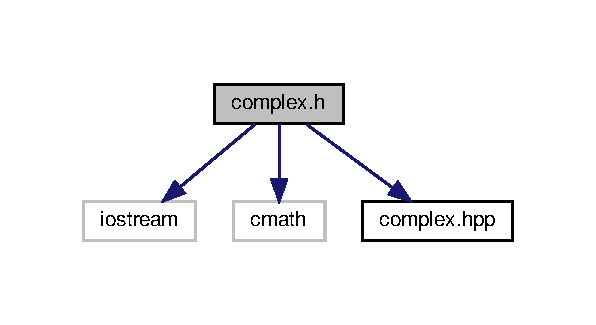
\includegraphics[width=286pt]{complex_8h__incl}
\end{center}
\end{figure}
This graph shows which files directly or indirectly include this file\+:\nopagebreak
\begin{figure}[H]
\begin{center}
\leavevmode
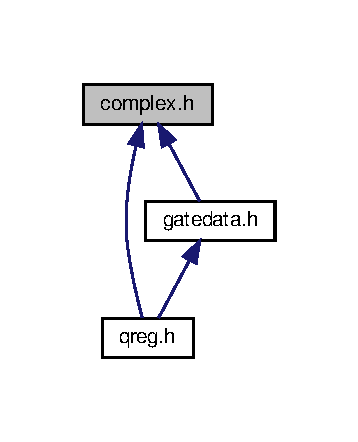
\includegraphics[width=172pt]{complex_8h__dep__incl}
\end{center}
\end{figure}
\subsection*{Classes}
\begin{DoxyCompactItemize}
\item 
class \hyperlink{classcomplex}{complex$<$ T $>$}
\begin{DoxyCompactList}\small\item\em complex class. \end{DoxyCompactList}\end{DoxyCompactItemize}
\subsection*{Functions}
\begin{DoxyCompactItemize}
\item 
{\footnotesize template$<$typename T $>$ }\\std\+::ostream \& \hyperlink{complex_8h_a7509b022f22e83b83303658565a038af}{operator$<$$<$} (std\+::ostream \&out, const \hyperlink{classcomplex}{complex}$<$ T $>$ \&rhs)
\begin{DoxyCompactList}\small\item\em Insertion operator. \end{DoxyCompactList}\end{DoxyCompactItemize}


\subsection{Detailed Description}
Definitions for the complex class. ~\newline
Programmer\+: Noah Klein ~\newline
Class\+: C\+S5201 ~\newline
Assignment\+: Homework 6 ~\newline


\subsection{Function Documentation}
\mbox{\Hypertarget{complex_8h_a7509b022f22e83b83303658565a038af}\label{complex_8h_a7509b022f22e83b83303658565a038af}} 
\index{complex.\+h@{complex.\+h}!operator$<$$<$@{operator$<$$<$}}
\index{operator$<$$<$@{operator$<$$<$}!complex.\+h@{complex.\+h}}
\subsubsection{\texorpdfstring{operator$<$$<$()}{operator<<()}}
{\footnotesize\ttfamily template$<$typename T $>$ \\
std\+::ostream\& operator$<$$<$ (\begin{DoxyParamCaption}\item[{std\+::ostream \&}]{out,  }\item[{const \hyperlink{classcomplex}{complex}$<$ T $>$ \&}]{rhs }\end{DoxyParamCaption})}



Insertion operator. 

Description\+: Insertion operator overload for the complex class that prints the object in the proper format. 
\begin{DoxyParams}{Parameters}
{\em out} & is the ostream passed to the function. \\
\hline
{\em rhs} & is the complex object to be output. \\
\hline
\end{DoxyParams}
\begin{DoxyReturn}{Returns}
Returns the ostream object. 
\end{DoxyReturn}
\begin{DoxyPrecond}{Precondition}
$<$$<$ operator must be defined for type T. 
\end{DoxyPrecond}
\begin{DoxyPostcond}{Postcondition}
The complex object is output to the stream. 
\end{DoxyPostcond}

\hypertarget{gatedata_8h}{}\section{gatedata.\+h File Reference}
\label{gatedata_8h}\index{gatedata.\+h@{gatedata.\+h}}
{\ttfamily \#include \char`\"{}n\+Trix.\+h\char`\"{}}\newline
{\ttfamily \#include \char`\"{}kronecker.\+h\char`\"{}}\newline
{\ttfamily \#include \char`\"{}complex.\+h\char`\"{}}\newline
{\ttfamily \#include \char`\"{}n\+Vect.\+h\char`\"{}}\newline
{\ttfamily \#include $<$iostream$>$}\newline
{\ttfamily \#include $<$algorithm$>$}\newline
{\ttfamily \#include $<$numeric$>$}\newline
Include dependency graph for gatedata.\+h\+:\nopagebreak
\begin{figure}[H]
\begin{center}
\leavevmode
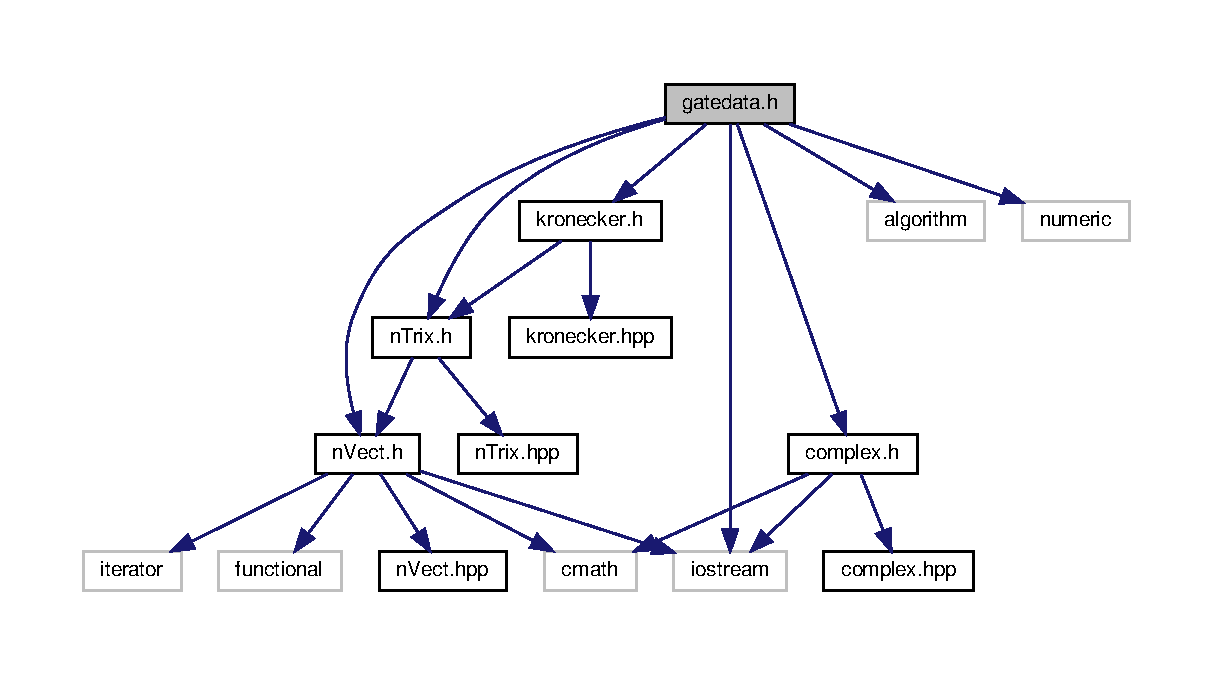
\includegraphics[width=350pt]{gatedata_8h__incl}
\end{center}
\end{figure}
This graph shows which files directly or indirectly include this file\+:\nopagebreak
\begin{figure}[H]
\begin{center}
\leavevmode
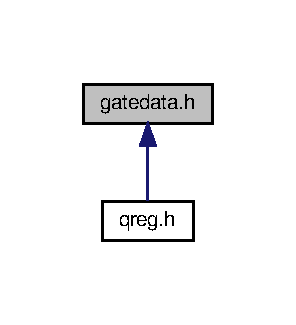
\includegraphics[width=142pt]{gatedata_8h__dep__incl}
\end{center}
\end{figure}
\subsection*{Classes}
\begin{DoxyCompactItemize}
\item 
class \hyperlink{classgatedata}{gatedata}
\begin{DoxyCompactList}\small\item\em complex class. \end{DoxyCompactList}\end{DoxyCompactItemize}
\subsection*{Typedefs}
\begin{DoxyCompactItemize}
\item 
typedef std\+::initializer\+\_\+list$<$ int $>$ \hyperlink{gatedata_8h_abecce716fb2428607e7c6cc3343d6c92}{listy}
\item 
typedef \hyperlink{classcomplex}{complex}$<$ float $>$ \hyperlink{gatedata_8h_a0c9667bfe3ded0fa2cd4fab281edbe24}{cpf}
\end{DoxyCompactItemize}


\subsection{Detailed Description}
Definitions for the gatedata class. ~\newline
Programmer\+: Noah Klein ~\newline
Class\+: C\+S5201 ~\newline
Assignment\+: Homework 6 ~\newline


\subsection{Typedef Documentation}
\mbox{\Hypertarget{gatedata_8h_a0c9667bfe3ded0fa2cd4fab281edbe24}\label{gatedata_8h_a0c9667bfe3ded0fa2cd4fab281edbe24}} 
\index{gatedata.\+h@{gatedata.\+h}!cpf@{cpf}}
\index{cpf@{cpf}!gatedata.\+h@{gatedata.\+h}}
\subsubsection{\texorpdfstring{cpf}{cpf}}
{\footnotesize\ttfamily typedef \hyperlink{classcomplex}{complex}$<$float$>$ \hyperlink{gatedata_8h_a0c9667bfe3ded0fa2cd4fab281edbe24}{cpf}}

shortened \hyperlink{classcomplex}{complex$<$float$>$} name \mbox{\Hypertarget{gatedata_8h_abecce716fb2428607e7c6cc3343d6c92}\label{gatedata_8h_abecce716fb2428607e7c6cc3343d6c92}} 
\index{gatedata.\+h@{gatedata.\+h}!listy@{listy}}
\index{listy@{listy}!gatedata.\+h@{gatedata.\+h}}
\subsubsection{\texorpdfstring{listy}{listy}}
{\footnotesize\ttfamily typedef std\+::initializer\+\_\+list$<$int$>$ \hyperlink{gatedata_8h_abecce716fb2428607e7c6cc3343d6c92}{listy}}

shortened list name 
\hypertarget{kronecker_8h}{}\section{kronecker.\+h File Reference}
\label{kronecker_8h}\index{kronecker.\+h@{kronecker.\+h}}
{\ttfamily \#include \char`\"{}n\+Trix.\+h\char`\"{}}\newline
{\ttfamily \#include \char`\"{}kronecker.\+hpp\char`\"{}}\newline
Include dependency graph for kronecker.\+h\+:\nopagebreak
\begin{figure}[H]
\begin{center}
\leavevmode
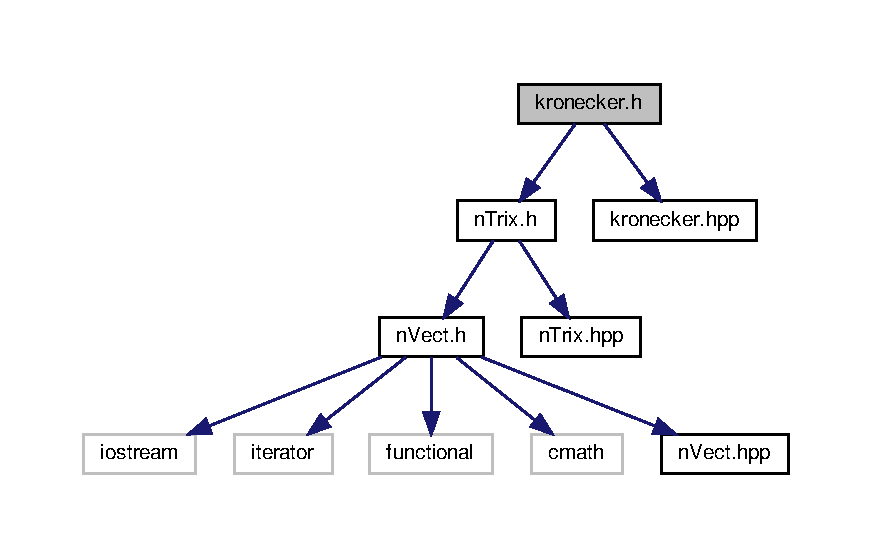
\includegraphics[width=350pt]{kronecker_8h__incl}
\end{center}
\end{figure}
This graph shows which files directly or indirectly include this file\+:\nopagebreak
\begin{figure}[H]
\begin{center}
\leavevmode
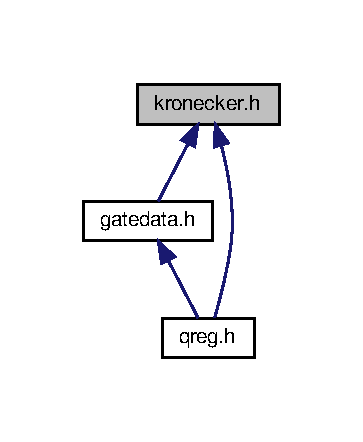
\includegraphics[width=174pt]{kronecker_8h__dep__incl}
\end{center}
\end{figure}
\subsection*{Classes}
\begin{DoxyCompactItemize}
\item 
class \hyperlink{classkronecker}{kronecker$<$ T $>$}
\begin{DoxyCompactList}\small\item\em kronecker class. \end{DoxyCompactList}\end{DoxyCompactItemize}


\subsection{Detailed Description}
Definitions for the kronecker class. ~\newline
Programmer\+: Noah Klein ~\newline
Class\+: C\+S5201 ~\newline
Assignment\+: Homework 6 ~\newline

\hypertarget{nTrix_8h}{}\section{n\+Trix.\+h File Reference}
\label{nTrix_8h}\index{n\+Trix.\+h@{n\+Trix.\+h}}
{\ttfamily \#include \char`\"{}n\+Vect.\+h\char`\"{}}\newline
{\ttfamily \#include \char`\"{}n\+Trix.\+hpp\char`\"{}}\newline
Include dependency graph for n\+Trix.\+h\+:\nopagebreak
\begin{figure}[H]
\begin{center}
\leavevmode
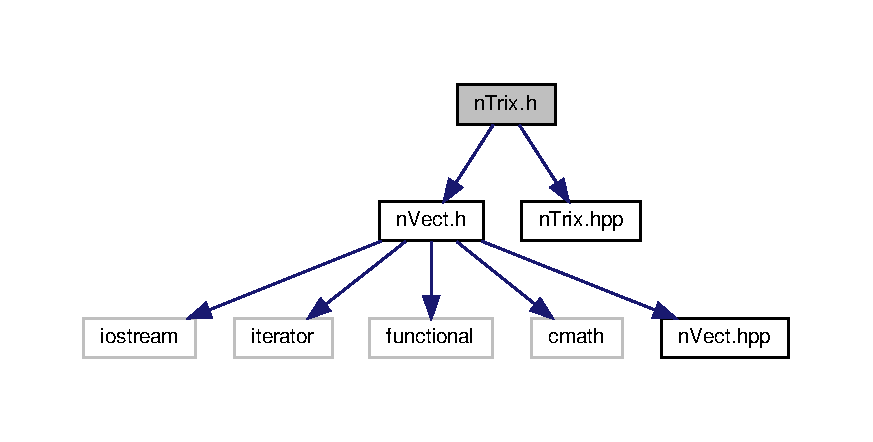
\includegraphics[width=350pt]{nTrix_8h__incl}
\end{center}
\end{figure}
This graph shows which files directly or indirectly include this file\+:\nopagebreak
\begin{figure}[H]
\begin{center}
\leavevmode
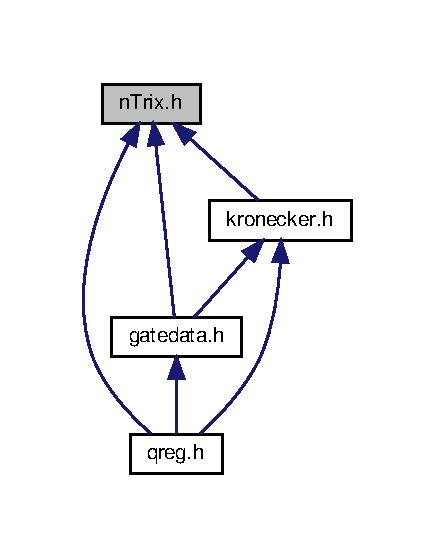
\includegraphics[width=209pt]{nTrix_8h__dep__incl}
\end{center}
\end{figure}
\subsection*{Classes}
\begin{DoxyCompactItemize}
\item 
class \hyperlink{classnTrix}{n\+Trix$<$ T $>$}
\begin{DoxyCompactList}\small\item\em \hyperlink{classnTrix}{n\+Trix} class. \end{DoxyCompactList}\end{DoxyCompactItemize}
\subsection*{Functions}
\begin{DoxyCompactItemize}
\item 
{\footnotesize template$<$typename T $>$ }\\std\+::ostream \& \hyperlink{nTrix_8h_a2bbb75cad63d3ba6e6f96960e09a58e2}{operator$<$$<$} (std\+::ostream \&out, const \hyperlink{classnTrix}{n\+Trix}$<$ T $>$ \&rhs)
\begin{DoxyCompactList}\small\item\em $<$$<$ operator \end{DoxyCompactList}\item 
{\footnotesize template$<$typename T $>$ }\\std\+::istream \& \hyperlink{nTrix_8h_ad36b0a966daad207c03f790ace312827}{operator$>$$>$} (std\+::istream \&in, \hyperlink{classnTrix}{n\+Trix}$<$ T $>$ \&rhs)
\begin{DoxyCompactList}\small\item\em \begin{quote}
\begin{quote}
operator\end{quote}
\end{quote}
\end{DoxyCompactList}\item 
{\footnotesize template$<$typename T $>$ }\\\hyperlink{classnTrix}{n\+Trix}$<$ T $>$ \hyperlink{nTrix_8h_aa6a9cd47a847b2f5567e13bd6c9c1fac}{operator$\ast$} (const \hyperlink{classnTrix}{n\+Trix}$<$ T $>$ \&lhs, const float scalar)
\begin{DoxyCompactList}\small\item\em 
\begin{DoxyItemize}
\item operator 
\end{DoxyItemize}\end{DoxyCompactList}\item 
{\footnotesize template$<$typename T $>$ }\\\hyperlink{classnTrix}{n\+Trix}$<$ T $>$ \hyperlink{nTrix_8h_abdb8062a93fea20839bdf926b1e16f94}{operator$\ast$} (const \hyperlink{classnVect}{n\+Vect}$<$ T $>$ \&lhs, const \hyperlink{classnTrix}{n\+Trix}$<$ T $>$ \&rhs)
\begin{DoxyCompactList}\small\item\em 
\begin{DoxyItemize}
\item operator 
\end{DoxyItemize}\end{DoxyCompactList}\item 
{\footnotesize template$<$typename T $>$ }\\\hyperlink{classnTrix}{n\+Trix}$<$ float $>$ \hyperlink{nTrix_8h_acb6ffe9fd3e8aa373a570884247ac35b}{r\+\_\+invert} (const \hyperlink{classnTrix}{n\+Trix}$<$ T $>$ \&A, \hyperlink{classnTrix}{n\+Trix}$<$ float $>$ \&B, \hyperlink{classnTrix}{n\+Trix}$<$ float $>$ \&E, const \hyperlink{classnTrix}{n\+Trix}$<$ float $>$ \&I, float Cerror, float Perror)
\begin{DoxyCompactList}\small\item\em recursive invert \end{DoxyCompactList}\end{DoxyCompactItemize}


\subsection{Detailed Description}
Definitions for the \hyperlink{classnTrix}{n\+Trix} class. ~\newline
Programmer\+: Noah Klein ~\newline
Class\+: C\+S5201 ~\newline
Assignment\+: Homework 6 ~\newline


\subsection{Function Documentation}
\mbox{\Hypertarget{nTrix_8h_aa6a9cd47a847b2f5567e13bd6c9c1fac}\label{nTrix_8h_aa6a9cd47a847b2f5567e13bd6c9c1fac}} 
\index{n\+Trix.\+h@{n\+Trix.\+h}!operator$\ast$@{operator$\ast$}}
\index{operator$\ast$@{operator$\ast$}!n\+Trix.\+h@{n\+Trix.\+h}}
\subsubsection{\texorpdfstring{operator$\ast$()}{operator*()}\hspace{0.1cm}{\footnotesize\ttfamily [1/2]}}
{\footnotesize\ttfamily template$<$typename T $>$ \\
\hyperlink{classnTrix}{n\+Trix}$<$T$>$ operator$\ast$ (\begin{DoxyParamCaption}\item[{const \hyperlink{classnTrix}{n\+Trix}$<$ T $>$ \&}]{lhs,  }\item[{const float}]{scalar }\end{DoxyParamCaption})}




\begin{DoxyItemize}
\item operator 
\end{DoxyItemize}

Description\+: Scalar multiplication for a n\+Trix$<$\+T$>$ object. 
\begin{DoxyParams}{Parameters}
{\em lhs} & is the n\+Trix$<$\+T$>$ object to be multiplied through. \\
\hline
{\em scalar} & is the scalar to multiply through the matrix. \\
\hline
\end{DoxyParams}
\begin{DoxyReturn}{Returns}
Returns a new n\+Trix$<$\+T$>$ object with the scalar multiplied throughout. 
\end{DoxyReturn}
\begin{DoxyPrecond}{Precondition}
$\ast$ operator must be defined for type T. 
\end{DoxyPrecond}
\mbox{\Hypertarget{nTrix_8h_abdb8062a93fea20839bdf926b1e16f94}\label{nTrix_8h_abdb8062a93fea20839bdf926b1e16f94}} 
\index{n\+Trix.\+h@{n\+Trix.\+h}!operator$\ast$@{operator$\ast$}}
\index{operator$\ast$@{operator$\ast$}!n\+Trix.\+h@{n\+Trix.\+h}}
\subsubsection{\texorpdfstring{operator$\ast$()}{operator*()}\hspace{0.1cm}{\footnotesize\ttfamily [2/2]}}
{\footnotesize\ttfamily template$<$typename T $>$ \\
\hyperlink{classnTrix}{n\+Trix}$<$T$>$ operator$\ast$ (\begin{DoxyParamCaption}\item[{const \hyperlink{classnVect}{n\+Vect}$<$ T $>$ \&}]{lhs,  }\item[{const \hyperlink{classnTrix}{n\+Trix}$<$ T $>$ \&}]{rhs }\end{DoxyParamCaption})}




\begin{DoxyItemize}
\item operator 
\end{DoxyItemize}

Description\+: $\ast$ operator overload for the \hyperlink{classnTrix}{n\+Trix} class that allows the user to multiply a matrix with a vector. 
\begin{DoxyParams}{Parameters}
{\em lhs} & is a \hyperlink{classnVect}{n\+Vect} object to be multiplied to a \hyperlink{classnTrix}{n\+Trix}. \\
\hline
{\em rhs} & is a \hyperlink{classnTrix}{n\+Trix} object to be multiplied to a \hyperlink{classnVect}{n\+Vect}. \\
\hline
\end{DoxyParams}
\begin{DoxyReturn}{Returns}
Returns a n\+Trix$<$\+T$>$ object with the proper dimensions and with the values having matrix multiplicaion applied. 
\end{DoxyReturn}
\begin{DoxyPrecond}{Precondition}
$\ast$ operator must be defined for type T. 
\end{DoxyPrecond}

\begin{DoxyExceptions}{Exceptions}
{\em Throws} & a std\+::invalid\+\_\+argument object if the two matrices are not the correct dimensions for matrix multiplication to occur. \\
\hline
\end{DoxyExceptions}
\mbox{\Hypertarget{nTrix_8h_a2bbb75cad63d3ba6e6f96960e09a58e2}\label{nTrix_8h_a2bbb75cad63d3ba6e6f96960e09a58e2}} 
\index{n\+Trix.\+h@{n\+Trix.\+h}!operator$<$$<$@{operator$<$$<$}}
\index{operator$<$$<$@{operator$<$$<$}!n\+Trix.\+h@{n\+Trix.\+h}}
\subsubsection{\texorpdfstring{operator$<$$<$()}{operator<<()}}
{\footnotesize\ttfamily template$<$typename T $>$ \\
std\+::ostream\& operator$<$$<$ (\begin{DoxyParamCaption}\item[{std\+::ostream \&}]{out,  }\item[{const \hyperlink{classnTrix}{n\+Trix}$<$ T $>$ \&}]{rhs }\end{DoxyParamCaption})}



$<$$<$ operator 

Description\+: $<$$<$ operator overloaded to pretty print the \hyperlink{classnTrix}{n\+Trix} object. 
\begin{DoxyParams}{Parameters}
{\em out} & is the ostream object passed to the function. \\
\hline
{\em rhs} & is the n\+Trix$<$\+T$>$ object to be output. \\
\hline
\end{DoxyParams}
\begin{DoxyReturn}{Returns}
Returns the ostream. 
\end{DoxyReturn}
\begin{DoxyPrecond}{Precondition}
$<$$<$ operator must be defined for type T. 
\end{DoxyPrecond}
\begin{DoxyPostcond}{Postcondition}
Outputs the matrix to the user. 
\end{DoxyPostcond}
\mbox{\Hypertarget{nTrix_8h_ad36b0a966daad207c03f790ace312827}\label{nTrix_8h_ad36b0a966daad207c03f790ace312827}} 
\index{n\+Trix.\+h@{n\+Trix.\+h}!operator$>$$>$@{operator$>$$>$}}
\index{operator$>$$>$@{operator$>$$>$}!n\+Trix.\+h@{n\+Trix.\+h}}
\subsubsection{\texorpdfstring{operator$>$$>$()}{operator>>()}}
{\footnotesize\ttfamily template$<$typename T $>$ \\
std\+::istream\& operator$>$$>$ (\begin{DoxyParamCaption}\item[{std\+::istream \&}]{in,  }\item[{\hyperlink{classnTrix}{n\+Trix}$<$ T $>$ \&}]{rhs }\end{DoxyParamCaption})}



\begin{quote}
\begin{quote}
operator\end{quote}
\end{quote}


Description\+: $>$$>$ operator overloaded to extract a matrix object from the istream. The inputted matrix overloads any previously stored data in the \hyperlink{classnTrix}{n\+Trix} object. 
\begin{DoxyParams}{Parameters}
{\em in} & is the istream object passed to the function. \\
\hline
{\em rhs} & is the n\+Trix$<$\+T$>$ object to store the input. \\
\hline
\end{DoxyParams}
\begin{DoxyReturn}{Returns}
Returns the istream. 
\end{DoxyReturn}
\begin{DoxyPrecond}{Precondition}
$>$$>$ operator must be defined for type T. 
\end{DoxyPrecond}
\begin{DoxyPostcond}{Postcondition}
Stores the input in the object passed. 
\end{DoxyPostcond}

\begin{DoxyExceptions}{Exceptions}
{\em Throws} & a std\+::range\+\_\+error object if the user inputs an incorrect number of items for a column. \\
\hline
\end{DoxyExceptions}
\mbox{\Hypertarget{nTrix_8h_acb6ffe9fd3e8aa373a570884247ac35b}\label{nTrix_8h_acb6ffe9fd3e8aa373a570884247ac35b}} 
\index{n\+Trix.\+h@{n\+Trix.\+h}!r\+\_\+invert@{r\+\_\+invert}}
\index{r\+\_\+invert@{r\+\_\+invert}!n\+Trix.\+h@{n\+Trix.\+h}}
\subsubsection{\texorpdfstring{r\+\_\+invert()}{r\_invert()}}
{\footnotesize\ttfamily template$<$typename T $>$ \\
\hyperlink{classnTrix}{n\+Trix}$<$float$>$ r\+\_\+invert (\begin{DoxyParamCaption}\item[{const \hyperlink{classnTrix}{n\+Trix}$<$ T $>$ \&}]{A,  }\item[{\hyperlink{classnTrix}{n\+Trix}$<$ float $>$ \&}]{B,  }\item[{\hyperlink{classnTrix}{n\+Trix}$<$ float $>$ \&}]{E,  }\item[{const \hyperlink{classnTrix}{n\+Trix}$<$ float $>$ \&}]{I,  }\item[{float}]{Cerror,  }\item[{float}]{Perror }\end{DoxyParamCaption})}



recursive invert 

Description\+: Recursive part of the invert function that iteratively calculates the inverse of a matrix. 
\begin{DoxyParams}{Parameters}
{\em A} & is the matrix that the user wants the inverse of. \\
\hline
{\em B} & is the previous version of one of the matrices needed in the iterative calculation. \\
\hline
{\em E} & is one of the matrices needed in the iterative calculation. \\
\hline
{\em I} & is the identity matrix in the proper dimension of the matrix A. \\
\hline
{\em Cerror} & is the current frobenius norm of matrix B. \\
\hline
{\em Perror} & is the previous frobenius norm of matrix B. \\
\hline
\end{DoxyParams}
\begin{DoxyReturn}{Returns}
Returns an inverted matrix A. 
\end{DoxyReturn}
\begin{DoxyPrecond}{Precondition}
=, -\/, and $\ast$ operators need to be defined for type T. 
\end{DoxyPrecond}

\hypertarget{nVect_8h}{}\section{n\+Vect.\+h File Reference}
\label{nVect_8h}\index{n\+Vect.\+h@{n\+Vect.\+h}}
{\ttfamily \#include $<$iostream$>$}\newline
{\ttfamily \#include $<$iterator$>$}\newline
{\ttfamily \#include $<$functional$>$}\newline
{\ttfamily \#include $<$cmath$>$}\newline
{\ttfamily \#include \char`\"{}n\+Vect.\+hpp\char`\"{}}\newline
Include dependency graph for n\+Vect.\+h\+:\nopagebreak
\begin{figure}[H]
\begin{center}
\leavevmode
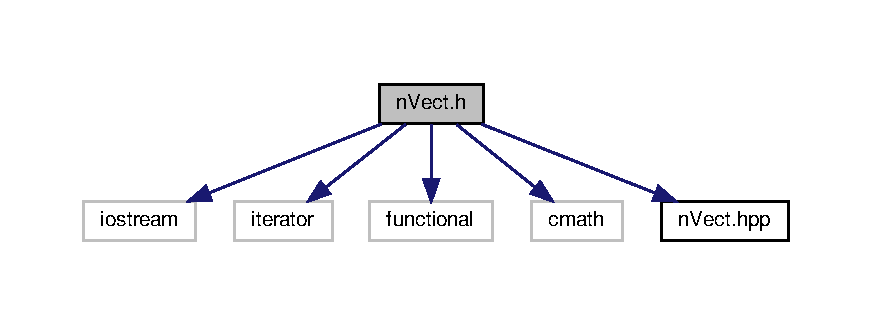
\includegraphics[width=350pt]{nVect_8h__incl}
\end{center}
\end{figure}
This graph shows which files directly or indirectly include this file\+:\nopagebreak
\begin{figure}[H]
\begin{center}
\leavevmode
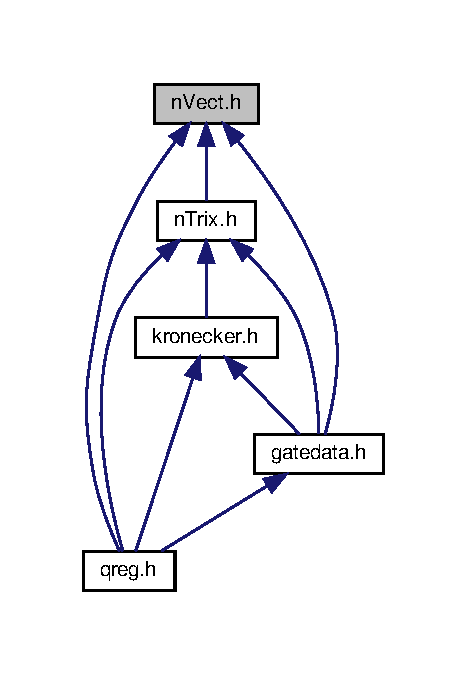
\includegraphics[width=224pt]{nVect_8h__dep__incl}
\end{center}
\end{figure}
\subsection*{Classes}
\begin{DoxyCompactItemize}
\item 
class \hyperlink{classnVect}{n\+Vect$<$ T $>$}
\begin{DoxyCompactList}\small\item\em \hyperlink{classnVect}{n\+Vect} class. \end{DoxyCompactList}\item 
class \hyperlink{classnVect_1_1iterator}{n\+Vect$<$ T $>$\+::iterator}
\begin{DoxyCompactList}\small\item\em iterator class. \end{DoxyCompactList}\end{DoxyCompactItemize}
\subsection*{Functions}
\begin{DoxyCompactItemize}
\item 
{\footnotesize template$<$typename T $>$ }\\\hyperlink{classnVect}{n\+Vect}$<$ T $>$ \hyperlink{nVect_8h_aaea4ae2e2f0c095902f38c22928c9d31}{operator+} (const \hyperlink{classnVect}{n\+Vect}$<$ T $>$ \&lhs, const \hyperlink{classnVect}{n\+Vect}$<$ T $>$ \&rhs)
\begin{DoxyCompactList}\small\item\em 
\begin{DoxyItemize}
\item operator 
\end{DoxyItemize}\end{DoxyCompactList}\item 
{\footnotesize template$<$typename T $>$ }\\\hyperlink{classnVect}{n\+Vect}$<$ T $>$ \hyperlink{nVect_8h_a8b1ac989f8040b056775eaeb81c506d2}{operator$\ast$} (const \hyperlink{classnVect}{n\+Vect}$<$ T $>$ \&lhs, const T \&rhs)
\begin{DoxyCompactList}\small\item\em Scalar multiplication. \end{DoxyCompactList}\item 
{\footnotesize template$<$typename T $>$ }\\\hyperlink{classnVect}{n\+Vect}$<$ T $>$ \hyperlink{nVect_8h_ab14d927799a17a9ecdaec6471fe51079}{operator$\ast$} (const T \&lhs, const \hyperlink{classnVect}{n\+Vect}$<$ T $>$ \&rhs)
\begin{DoxyCompactList}\small\item\em Scalar multiplication. \end{DoxyCompactList}\item 
{\footnotesize template$<$typename T $>$ }\\std\+::ostream \& \hyperlink{nVect_8h_ac41f0d1072a4da1e6b7e1c0139d7edaa}{operator$<$$<$} (std\+::ostream \&out, const \hyperlink{classnVect}{n\+Vect}$<$ T $>$ \&rhs)
\begin{DoxyCompactList}\small\item\em $<$$<$ operator \end{DoxyCompactList}\item 
{\footnotesize template$<$typename T $>$ }\\std\+::istream \& \hyperlink{nVect_8h_a633c2e020b48c20b53f449795b64317d}{operator$>$$>$} (std\+::istream \&in, \hyperlink{classnVect}{n\+Vect}$<$ T $>$ \&rhs)
\begin{DoxyCompactList}\small\item\em \begin{quote}
\begin{quote}
operator\end{quote}
\end{quote}
\end{DoxyCompactList}\end{DoxyCompactItemize}


\subsection{Detailed Description}
Definitions for the \hyperlink{classnVect}{n\+Vect} class. ~\newline
Programmer\+: Noah Klein ~\newline
Class\+: C\+S5201 ~\newline
Assignment\+: Homework 6 ~\newline


\subsection{Function Documentation}
\mbox{\Hypertarget{nVect_8h_a8b1ac989f8040b056775eaeb81c506d2}\label{nVect_8h_a8b1ac989f8040b056775eaeb81c506d2}} 
\index{n\+Vect.\+h@{n\+Vect.\+h}!operator$\ast$@{operator$\ast$}}
\index{operator$\ast$@{operator$\ast$}!n\+Vect.\+h@{n\+Vect.\+h}}
\subsubsection{\texorpdfstring{operator$\ast$()}{operator*()}\hspace{0.1cm}{\footnotesize\ttfamily [1/2]}}
{\footnotesize\ttfamily template$<$typename T $>$ \\
\hyperlink{classnVect}{n\+Vect}$<$T$>$ operator$\ast$ (\begin{DoxyParamCaption}\item[{const \hyperlink{classnVect}{n\+Vect}$<$ T $>$ \&}]{lhs,  }\item[{const T \&}]{rhs }\end{DoxyParamCaption})}



Scalar multiplication. 

Description\+: Allows for scalar multiplication of a calling vector. 
\begin{DoxyParams}{Parameters}
{\em lhs} & is the \hyperlink{classnVect}{n\+Vect} that the scalar will be multiplied through. \\
\hline
{\em rhs} & is a scalar of type T to be multiplied through the vector. \\
\hline
\end{DoxyParams}
\begin{DoxyReturn}{Returns}
Returns a newly created vector where the data in each container has been multiplied by the scalar. 
\end{DoxyReturn}
\begin{DoxyPrecond}{Precondition}
$\ast$= operator needs to be defined for type T. 
\end{DoxyPrecond}
\begin{DoxyPostcond}{Postcondition}
Creates a new vector that gets returned. 
\end{DoxyPostcond}
\mbox{\Hypertarget{nVect_8h_ab14d927799a17a9ecdaec6471fe51079}\label{nVect_8h_ab14d927799a17a9ecdaec6471fe51079}} 
\index{n\+Vect.\+h@{n\+Vect.\+h}!operator$\ast$@{operator$\ast$}}
\index{operator$\ast$@{operator$\ast$}!n\+Vect.\+h@{n\+Vect.\+h}}
\subsubsection{\texorpdfstring{operator$\ast$()}{operator*()}\hspace{0.1cm}{\footnotesize\ttfamily [2/2]}}
{\footnotesize\ttfamily template$<$typename T $>$ \\
\hyperlink{classnVect}{n\+Vect}$<$T$>$ operator$\ast$ (\begin{DoxyParamCaption}\item[{const T \&}]{lhs,  }\item[{const \hyperlink{classnVect}{n\+Vect}$<$ T $>$ \&}]{rhs }\end{DoxyParamCaption})}



Scalar multiplication. 

Description\+: Allows for scalar multiplication of a calling vector. 
\begin{DoxyParams}{Parameters}
{\em lhs} & is a \hyperlink{classnVect}{n\+Vect} that the scalar will be muliplied through. \\
\hline
{\em rhs} & is a scalar of type T to be multiplied through the vector. \\
\hline
\end{DoxyParams}
\begin{DoxyReturn}{Returns}
Returns a newly created vector where the data in each container has been multiplied by the scalar. 
\end{DoxyReturn}
\begin{DoxyPrecond}{Precondition}
$\ast$= operator needs to be defined for type T. 
\end{DoxyPrecond}
\begin{DoxyPostcond}{Postcondition}
Creates a new vector that gets returned. 
\end{DoxyPostcond}
\mbox{\Hypertarget{nVect_8h_aaea4ae2e2f0c095902f38c22928c9d31}\label{nVect_8h_aaea4ae2e2f0c095902f38c22928c9d31}} 
\index{n\+Vect.\+h@{n\+Vect.\+h}!operator+@{operator+}}
\index{operator+@{operator+}!n\+Vect.\+h@{n\+Vect.\+h}}
\subsubsection{\texorpdfstring{operator+()}{operator+()}}
{\footnotesize\ttfamily template$<$typename T $>$ \\
\hyperlink{classnVect}{n\+Vect}$<$T$>$ operator+ (\begin{DoxyParamCaption}\item[{const \hyperlink{classnVect}{n\+Vect}$<$ T $>$ \&}]{lhs,  }\item[{const \hyperlink{classnVect}{n\+Vect}$<$ T $>$ \&}]{rhs }\end{DoxyParamCaption})}




\begin{DoxyItemize}
\item operator 
\end{DoxyItemize}

Description\+: Used to add two vectors together. Allows for vectors of different (or similar) sizes to be added through vector addition. 
\begin{DoxyParams}{Parameters}
{\em lhs} & is the \hyperlink{classnVect}{n\+Vect} to be added to. \\
\hline
{\em rhs} & is the \hyperlink{classnVect}{n\+Vect} to be added to the calling object. \\
\hline
\end{DoxyParams}
\begin{DoxyReturn}{Returns}
Returns a newly created vector where each container now holds the sum of the two vectors passed at that index. 
\end{DoxyReturn}
\begin{DoxyPrecond}{Precondition}
+= operator needs to be defined for type T. 
\end{DoxyPrecond}
\begin{DoxyPostcond}{Postcondition}
Creates a new vector that gets returned. 
\end{DoxyPostcond}
\mbox{\Hypertarget{nVect_8h_ac41f0d1072a4da1e6b7e1c0139d7edaa}\label{nVect_8h_ac41f0d1072a4da1e6b7e1c0139d7edaa}} 
\index{n\+Vect.\+h@{n\+Vect.\+h}!operator$<$$<$@{operator$<$$<$}}
\index{operator$<$$<$@{operator$<$$<$}!n\+Vect.\+h@{n\+Vect.\+h}}
\subsubsection{\texorpdfstring{operator$<$$<$()}{operator<<()}}
{\footnotesize\ttfamily template$<$typename T $>$ \\
std\+::ostream\& operator$<$$<$ (\begin{DoxyParamCaption}\item[{std\+::ostream \&}]{out,  }\item[{const \hyperlink{classnVect}{n\+Vect}$<$ T $>$ \&}]{rhs }\end{DoxyParamCaption})}



$<$$<$ operator 

Description\+: Allows for proper outputting of \hyperlink{classnVect}{n\+Vect} objects. 
\begin{DoxyParams}{Parameters}
{\em out} & is the ostream passed. \\
\hline
{\em rhs} & is the \hyperlink{classnVect}{n\+Vect} to be output. \\
\hline
\end{DoxyParams}
\begin{DoxyReturn}{Returns}
Returns the ostream 
\end{DoxyReturn}
\begin{DoxyPrecond}{Precondition}
$<$$<$ operator must be defined for type T. 
\end{DoxyPrecond}
\begin{DoxyPostcond}{Postcondition}
Outputs the object to the stream. 
\end{DoxyPostcond}
\mbox{\Hypertarget{nVect_8h_a633c2e020b48c20b53f449795b64317d}\label{nVect_8h_a633c2e020b48c20b53f449795b64317d}} 
\index{n\+Vect.\+h@{n\+Vect.\+h}!operator$>$$>$@{operator$>$$>$}}
\index{operator$>$$>$@{operator$>$$>$}!n\+Vect.\+h@{n\+Vect.\+h}}
\subsubsection{\texorpdfstring{operator$>$$>$()}{operator>>()}}
{\footnotesize\ttfamily template$<$typename T $>$ \\
std\+::istream\& operator$>$$>$ (\begin{DoxyParamCaption}\item[{std\+::istream \&}]{in,  }\item[{\hyperlink{classnVect}{n\+Vect}$<$ T $>$ \&}]{rhs }\end{DoxyParamCaption})}



\begin{quote}
\begin{quote}
operator\end{quote}
\end{quote}


Description\+: Allows the user to insert any amount of data into a \hyperlink{classnVect}{n\+Vect} object. 
\begin{DoxyParams}{Parameters}
{\em in} & is the istream passed. \\
\hline
{\em rhs} & is the \hyperlink{classnVect}{n\+Vect} to store input. \\
\hline
\end{DoxyParams}
\begin{DoxyReturn}{Returns}
Returns the istream. 
\end{DoxyReturn}
\begin{DoxyPostcond}{Postcondition}
Inputted data is stored in the rhs \hyperlink{classnVect}{n\+Vect}. 
\end{DoxyPostcond}

\hypertarget{qreg_8h}{}\section{qreg.\+h File Reference}
\label{qreg_8h}\index{qreg.\+h@{qreg.\+h}}
{\ttfamily \#include \char`\"{}n\+Vect.\+h\char`\"{}}\newline
{\ttfamily \#include \char`\"{}complex.\+h\char`\"{}}\newline
{\ttfamily \#include \char`\"{}gatedata.\+h\char`\"{}}\newline
{\ttfamily \#include \char`\"{}n\+Trix.\+h\char`\"{}}\newline
{\ttfamily \#include \char`\"{}kronecker.\+h\char`\"{}}\newline
{\ttfamily \#include \char`\"{}qreg.\+hpp\char`\"{}}\newline
Include dependency graph for qreg.\+h\+:\nopagebreak
\begin{figure}[H]
\begin{center}
\leavevmode
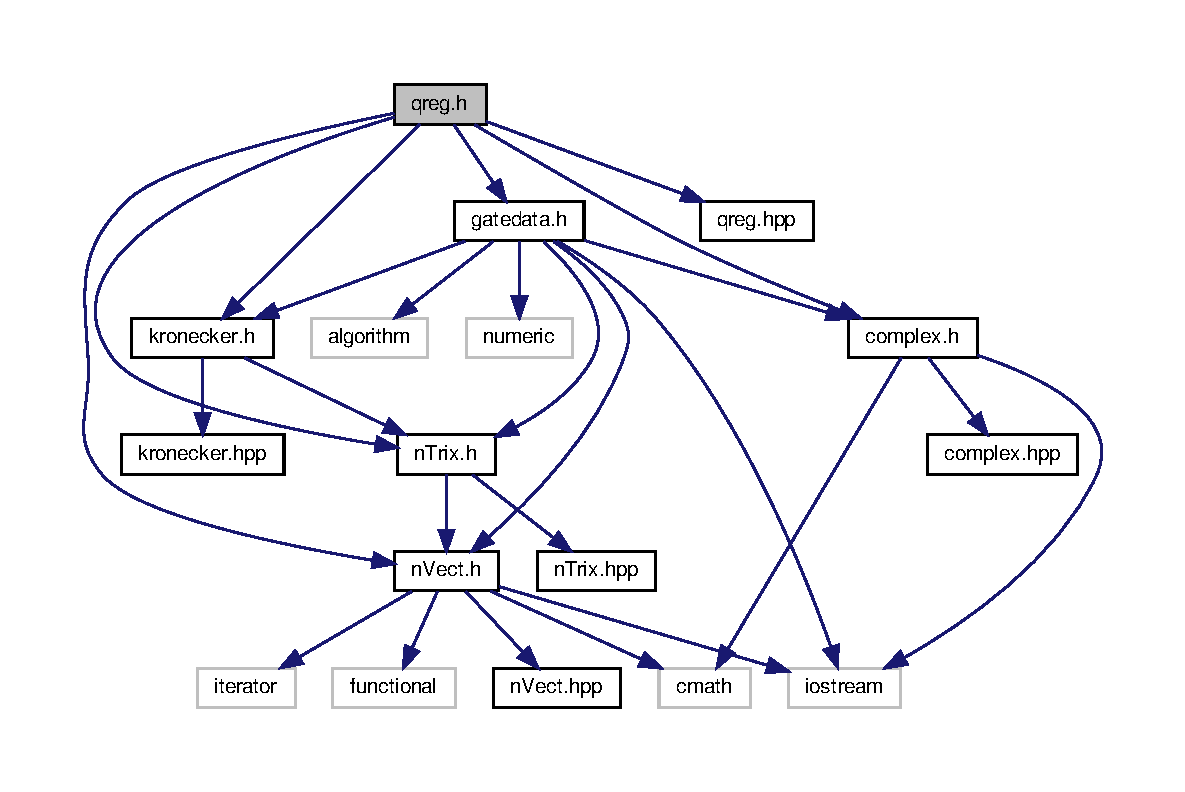
\includegraphics[width=350pt]{qreg_8h__incl}
\end{center}
\end{figure}
\subsection*{Classes}
\begin{DoxyCompactItemize}
\item 
class \hyperlink{classqreg}{qreg$<$ size $>$}
\begin{DoxyCompactList}\small\item\em qreg class. \end{DoxyCompactList}\end{DoxyCompactItemize}
\subsection*{Functions}
\begin{DoxyCompactItemize}
\item 
{\footnotesize template$<$int size$>$ }\\std\+::ostream \& \hyperlink{qreg_8h_a52f1eed320cfd61ac0a63f9e258e0c1c}{operator$<$$<$} (std\+::ostream \&out, \hyperlink{classqreg}{qreg}$<$ size $>$ \&rhs)
\begin{DoxyCompactList}\small\item\em operator $<$$<$ \end{DoxyCompactList}\end{DoxyCompactItemize}


\subsection{Detailed Description}
Definitions for the quantum register class. ~\newline
Programmer\+: Noah Klein ~\newline
Class\+: C\+S5201 ~\newline
Assignment\+: Homework 6 ~\newline


\subsection{Function Documentation}
\mbox{\Hypertarget{qreg_8h_a52f1eed320cfd61ac0a63f9e258e0c1c}\label{qreg_8h_a52f1eed320cfd61ac0a63f9e258e0c1c}} 
\index{qreg.\+h@{qreg.\+h}!operator$<$$<$@{operator$<$$<$}}
\index{operator$<$$<$@{operator$<$$<$}!qreg.\+h@{qreg.\+h}}
\subsubsection{\texorpdfstring{operator$<$$<$()}{operator<<()}}
{\footnotesize\ttfamily template$<$int size$>$ \\
std\+::ostream\& operator$<$$<$ (\begin{DoxyParamCaption}\item[{std\+::ostream \&}]{out,  }\item[{\hyperlink{classqreg}{qreg}$<$ size $>$ \&}]{rhs }\end{DoxyParamCaption})}



operator $<$$<$ 

Description\+: Insertion operator overload for the qreg class that measures the state of the system and outputs it in the proper format. 
\begin{DoxyParams}{Parameters}
{\em out} & is the ostream object. \\
\hline
{\em rhs} & is the qreg object to be output. \\
\hline
\end{DoxyParams}
\begin{DoxyPrecond}{Precondition}
If the probability of a state is less than .00001, this is interpreted as 0 to assist with floating point error. 
\end{DoxyPrecond}
\begin{DoxyPostcond}{Postcondition}
The state is measured and output accordingly. If the system is measured again it will output the same information. 
\end{DoxyPostcond}

%--- End generated contents ---

% Index
\backmatter
\newpage
\phantomsection
\clearemptydoublepage
\addcontentsline{toc}{chapter}{Index}
\printindex

\end{document}
